%%%%%%%%%%%%%%%%%%%%%%%%%%%%%%%%%%%%%%%%%
% Beamer Presentation
% LaTeX Template
% Version 1.0 (10/11/12)
%
% This template has been downloaded from:
% http://www.LaTeXTemplates.com
%
% License:
% CC BY-NC-SA 3.0 (http://creativecommons.org/licenses/by-nc-sa/3.0/)
%
%%%%%%%%%%%%%%%%%%%%%%%%%%%%%%%%%%%%%%%%%

%----------------------------------------------------------------------------------------
%	PACKAGES AND THEMES
%----------------------------------------------------------------------------------------

\documentclass{beamer}

\mode<presentation> {

% The Beamer class comes with a number of default slide themes
% which change the colors and layouts of slides. Below this is a list
% of all the themes, uncomment each in turn to see what they look like.

%\usetheme{default}
%\usetheme{AnnArbor}
%\usetheme{Antibes}
%\usetheme{Bergen}
%\usetheme{Berkeley}
%\usetheme{Berlin}
%\usetheme{Boadilla}
%\usetheme{CambridgeUS}
%\usetheme{Copenhagen}
%\usetheme{Darmstadt}
%\usetheme{Dresden}
%\usetheme{Frankfurt}
%\usetheme{Goettingen}
%\usetheme{Hannover}
%\usetheme{Ilmenau}
%\usetheme{JuanLesPins}
%\usetheme{Luebeck}
\usetheme{Madrid}
%\usetheme{Malmoe}
%\usetheme{Marburg}
%\usetheme{Montpellier}
%\usetheme{PaloAlto}
%\usetheme{Pittsburgh}
%\usetheme{Rochester}
%\usetheme{Singapore}
%\usetheme{Szeged}
%\usetheme{Warsaw}

% As well as themes, the Beamer class has a number of color themes
% for any slide theme. Uncomment each of these in turn to see how it
% changes the colors of your current slide theme.

%\usecolortheme{albatross}
\usecolortheme{beaver}
%\usecolortheme{beetle}
%\usecolortheme{crane}
%\usecolortheme{dolphin}
%\usecolortheme{dove}
%\usecolortheme{fly}
%\usecolortheme{lily}
%\usecolortheme{orchid}
%\usecolortheme{rose}
%\usecolortheme{seagull}
%\usecolortheme{seahorse}
%\usecolortheme{whale}
%\usecolortheme{wolverine}

%\setbeamertemplate{footline} % To remove the footer line in all slides uncomment this line
%\setbeamertemplate{footline}[page number] % To replace the footer line in all slides with a simple slide count uncomment this line

%\setbeamertemplate{navigation symbols}{} % To remove the navigation symbols from the bottom of all slides uncomment this line

\setbeamertemplate{frametitle}[default][center]
}

\usepackage{graphicx} % Allows including images
\usepackage{booktabs} % Allows the use of \toprule, \midrule and \bottomrule in tables
\usepackage{multimedia}
%\usepackage{movie15}
\usepackage{caption}
\usepackage{subcaption}
\usepackage{amsfonts}
\usepackage{epstopdf}
\usepackage{bigints}
\usepackage{amsmath}
\usepackage{hyperref}
\usepackage{verbatim}
\usepackage{mathrsfs}
\usepackage{color}
\usepackage[outline]{contour}
\usepackage{multirow}

\contourlength{1pt}

\newcommand\Bo{\mbox{\textit{Bo}}}  % Bond number
\newcommand\Rey{\mbox{\textit{Re}}}  % Reynolds number
\newcommand\Ri{\mbox{\textit{Ri}}}  % Richardson number

\def\Xint#1{\mathchoice
{\XXint\displaystyle\textstyle{#1}}%
{\XXint\textstyle\scriptstyle{#1}}%
{\XXint\scriptstyle\scriptscriptstyle{#1}}%
{\XXint\scriptscriptstyle\scriptscriptstyle{#1}}%
\!\int}
\def\XXint#1#2#3{{\setbox0=\hbox{$#1{#2#3}{\int}$}
\vcenter{\hbox{$#2#3$}}\kern-.5\wd0}}
\def\ddashint{\Xint=}
\def\dashint{\Xint-}

%----------------------------------------------------------------------------------------
%	TITLE PAGE
%----------------------------------------------------------------------------------------

\title[Modeling volcanic processes]{Gravity currents} % The short title appears at the bottom of every slide, the full title is only on the title page

\author[Paul Jarvis]{Paul A. Jarvis} % Your name
\institute[UNIGE] % Your institution as it will appear on the bottom of every slide, may be shorthand to save space
{
\textit{paul.jarvis@unige.ch} % Your email address
}
\date{22nd November 2019} % Date, can be changed to a custom date
\begin{columns}

  \begin{column}{0.33\paperwidth}
    $$
\includegraphics[width=0.3\paperwidth]{UNIGE_logo.jpg}$$
  \end{column}

  \begin{column}{0.33\paperwidth}
    $$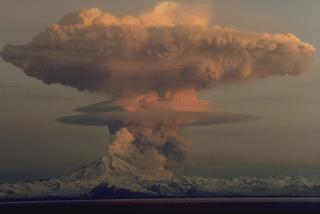
\includegraphics[width=0.3\paperwidth]{redoubt.jpg}$$
  \end{column}

  \begin{column}{0.33\paperwidth}
    $$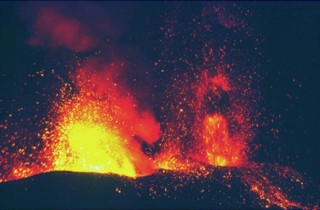
\includegraphics[width=0.3\paperwidth]{etna.jpg}$$
  \end{column}
  
\end{columns}
\vspace{-2cm}

\DeclareMathOperator\erf{erf}

\begin{document}

\begin{frame}
\titlepage % Print the title page as the first slide
\end{frame}

%\begin{frame}
%\frametitle{Overview} % Table of contents slide, comment this block out to remove it
%\tableofcontents % Throughout your presentation, if you choose to use \section{} and \subsection{} commands, these will automatically be printed on this slide as an overview of your presentation
%\end{frame}


%----------------------------------------------------------------------------------------
%	PRESENTATION SLIDES
%----------------------------------------------------------------------------------------

%------------------------------------------------
%\section{First Section} % Sections can be created in order to organize your presentation into discrete blocks, all sections and subsections are automatically printed in the table of contents as an overview of the talk
%------------------------------------------------

%\subsection{Subsection Example} % A subsection can be created just before a set of slides with a common theme to further break down your presentation into chunks

\begin{frame}
  \frametitle{Volcanic flows}

  \vspace{-0.6cm}
  
  \begin{columns}[t]

    \begin{column}{0.5\paperwidth}

      \centering \textbf{Lava flows}

      \vspace{-0.6cm}
      
      $$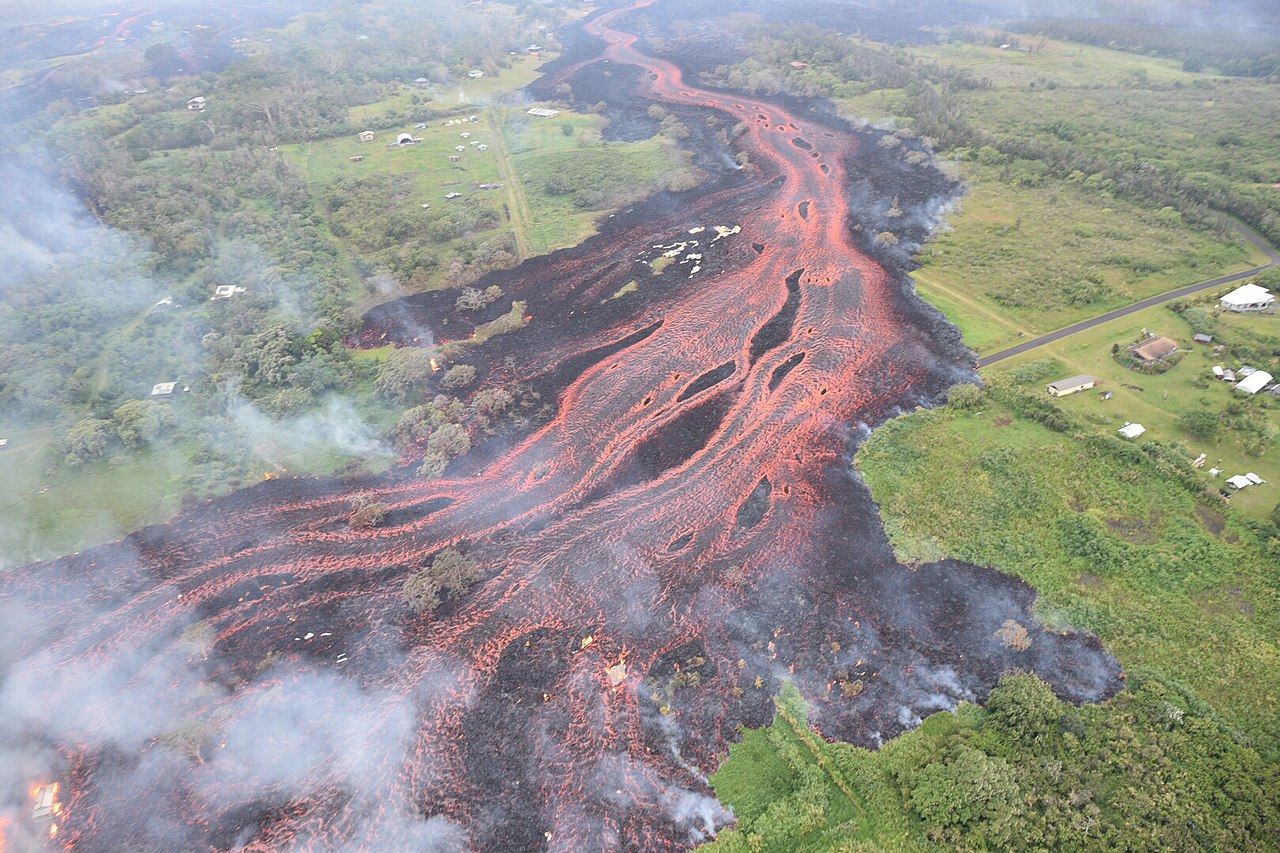
\includegraphics[width=0.8\textwidth]{flow.jpg}$$

      \vspace{-0.5cm}

      \textbf{Pyroclastic density currents (PDCs)}

      \vspace{-0.6cm}

      $$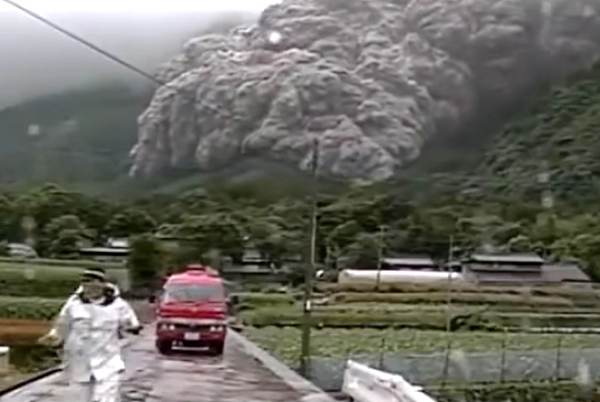
\includegraphics[width=0.8\textwidth]{pdc.jpg}$$      
      
    \end{column}

    \begin{column}{0.5\paperwidth}

      \centering \textbf{Cloud spreading}

      \vspace{-0.6cm}

      $$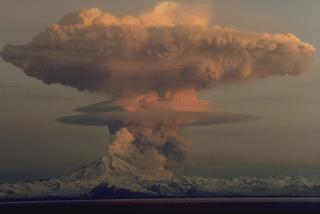
\includegraphics[width=0.8\textwidth]{redoubt.jpg}$$

      \vspace{-0.5cm}

      \textbf{Lahars}

      \vspace{-0.6cm}

      $$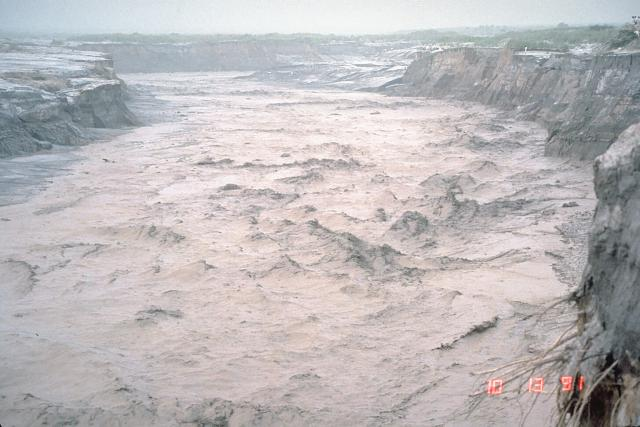
\includegraphics[width=0.8\textwidth]{lahar.jpg}$$
      
    \end{column}
    
  \end{columns}
  
\end{frame}
%-----------------------------------------------
\begin{frame}
  \frametitle{Hydrostatic gradients}

  \begin{columns}[t]

    \begin{column}{0.5\paperwidth}

      \vspace{-1cm}
      
      $$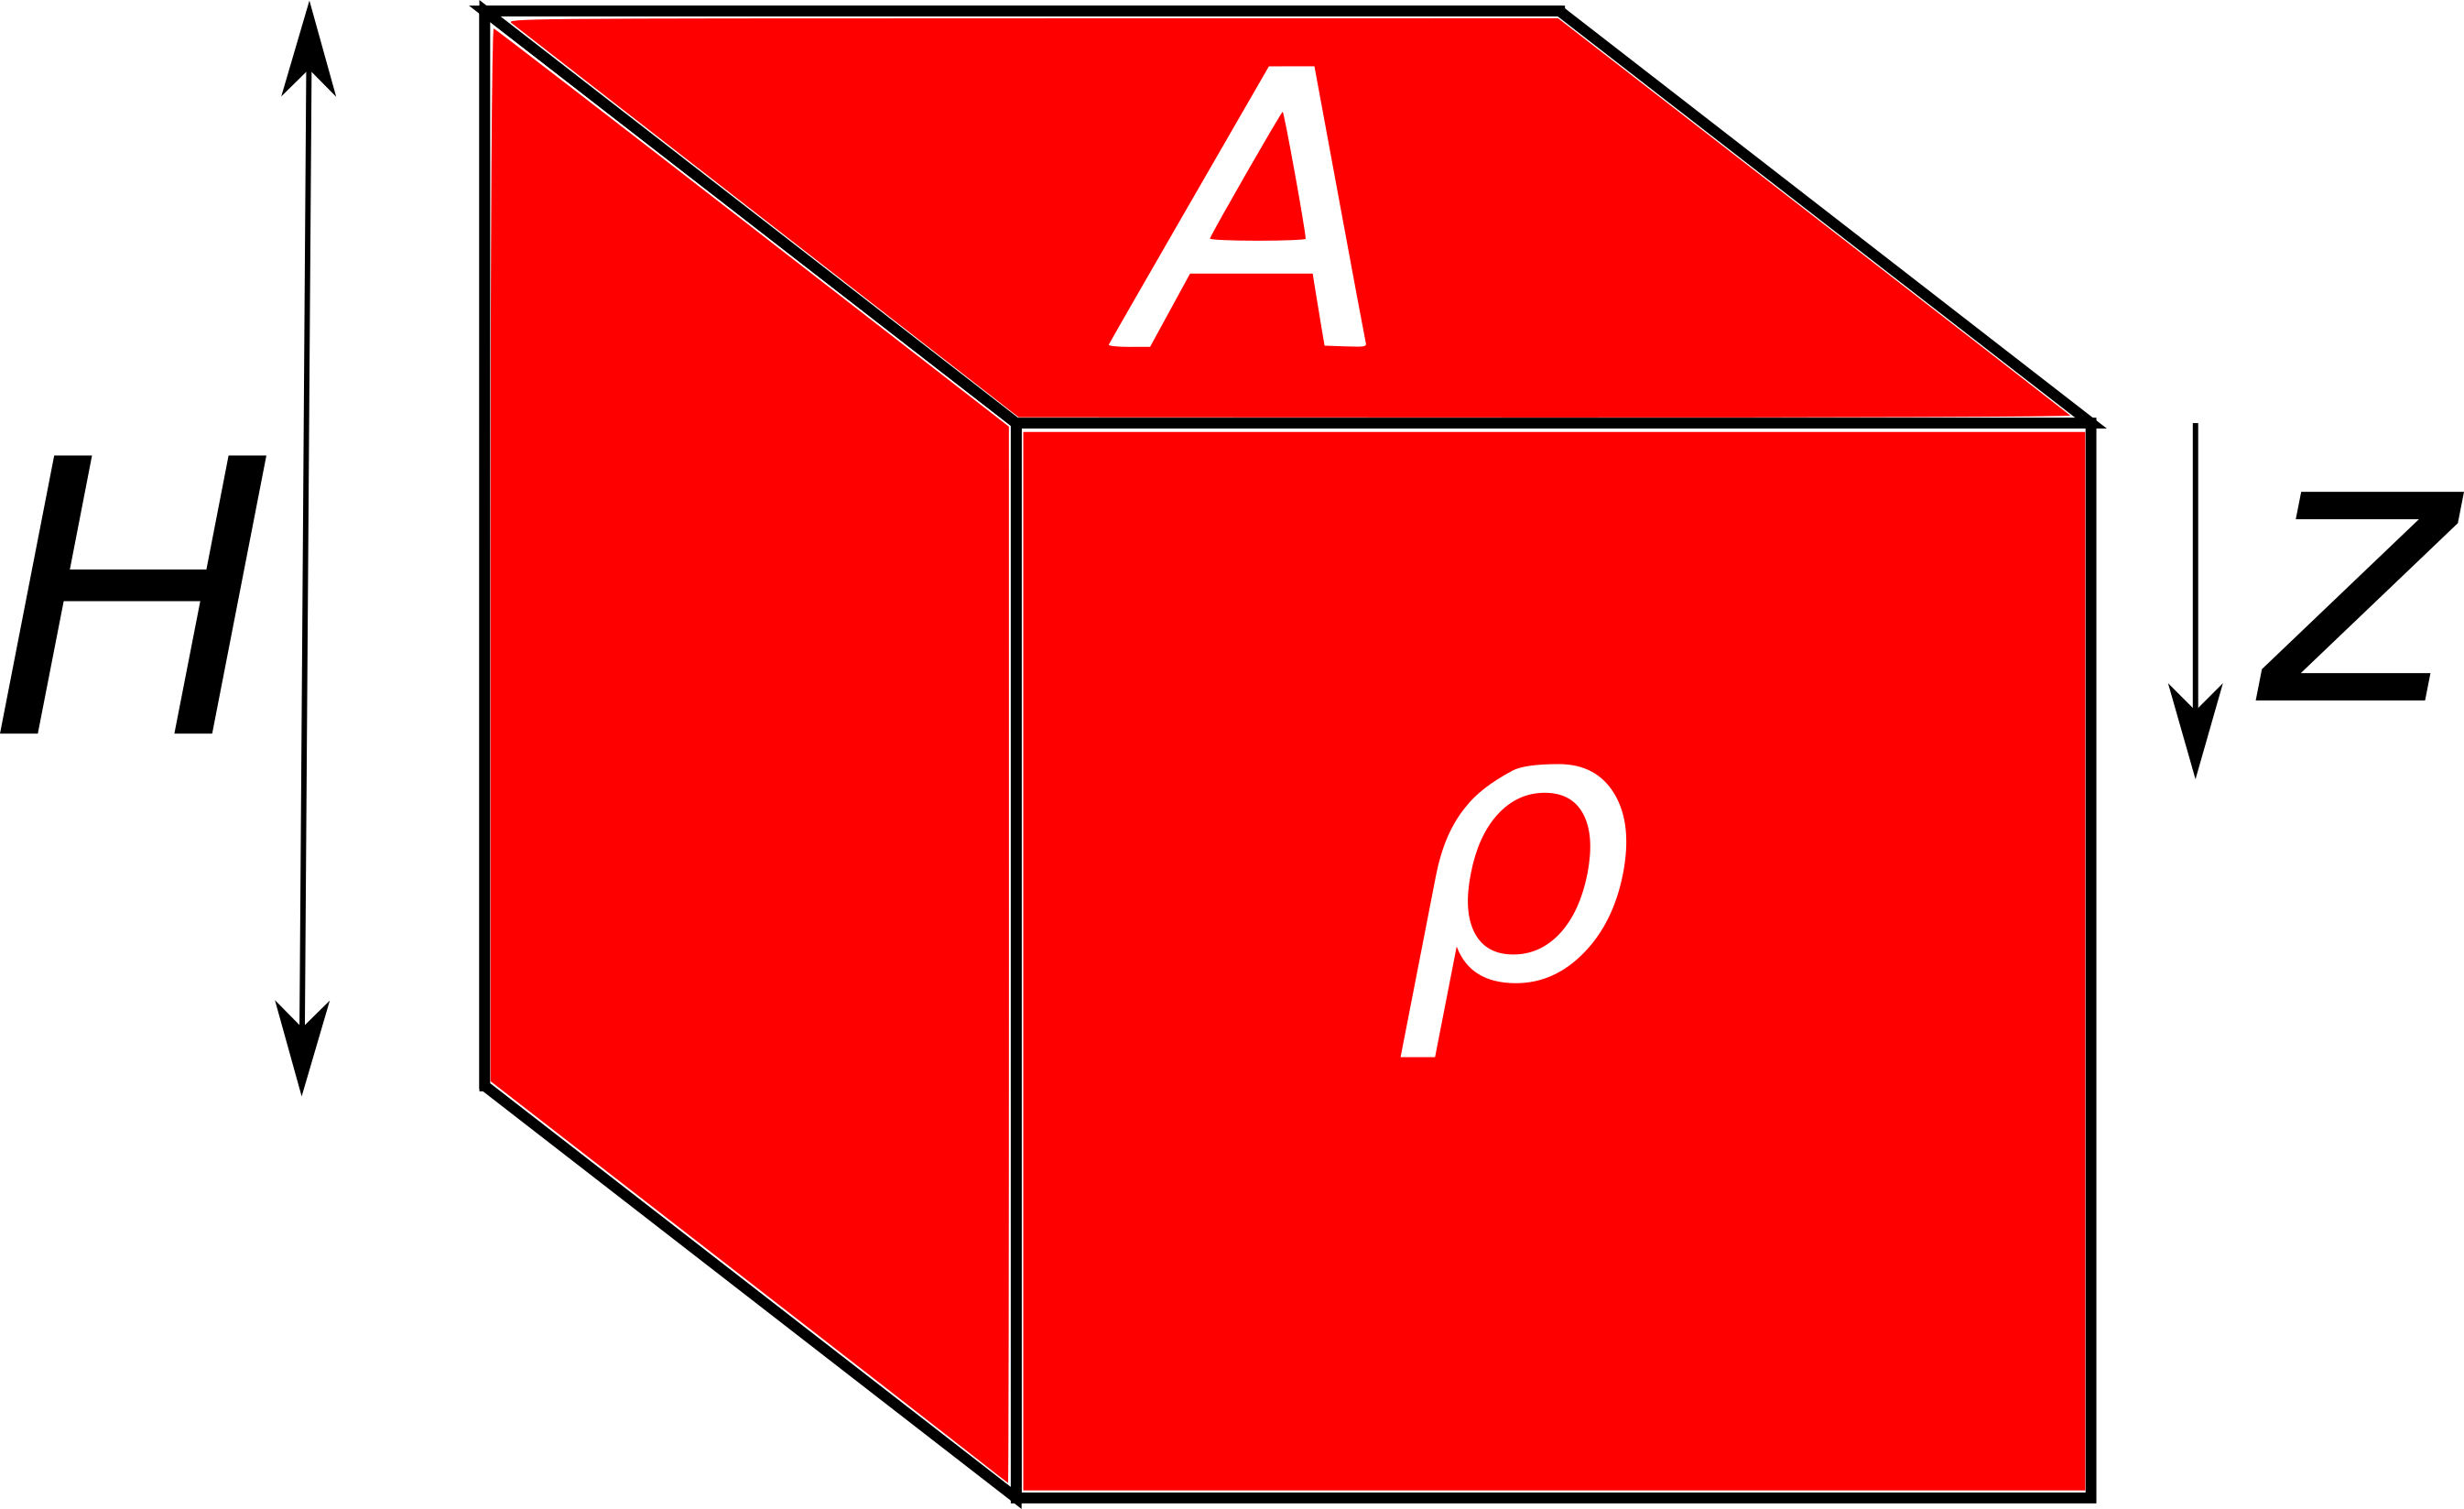
\includegraphics[width=0.8\textwidth]{column.png}$$

      Consider horizontal plane at depth $z$ \\

      What are the forces acting on this plane? \\

      \begin{itemize}
      \item \textbf{Weight} of overlying fluid \\
        \vspace{-0.5cm}
        $$ W = \rho A z g$$
      \item Balanced by \textbf{hydrostatic pressure} \\
        \vspace{-0.5cm}
        $$ F_{\text{p}} = P A $$
      \end{itemize}
    \end{column}

    \begin{column}{0.49\paperwidth}

      \vspace{-0.5cm}
      
      Consider a volume of fluid of :

      \begin{itemize}
      \item Density $\rho$ \\
      \item Height $H$ \\
      \item Horizontal cross section $A$ \\
      \end{itemize}

      $z$ = Negative vertical coordinate (depth below top surface) \\

      $$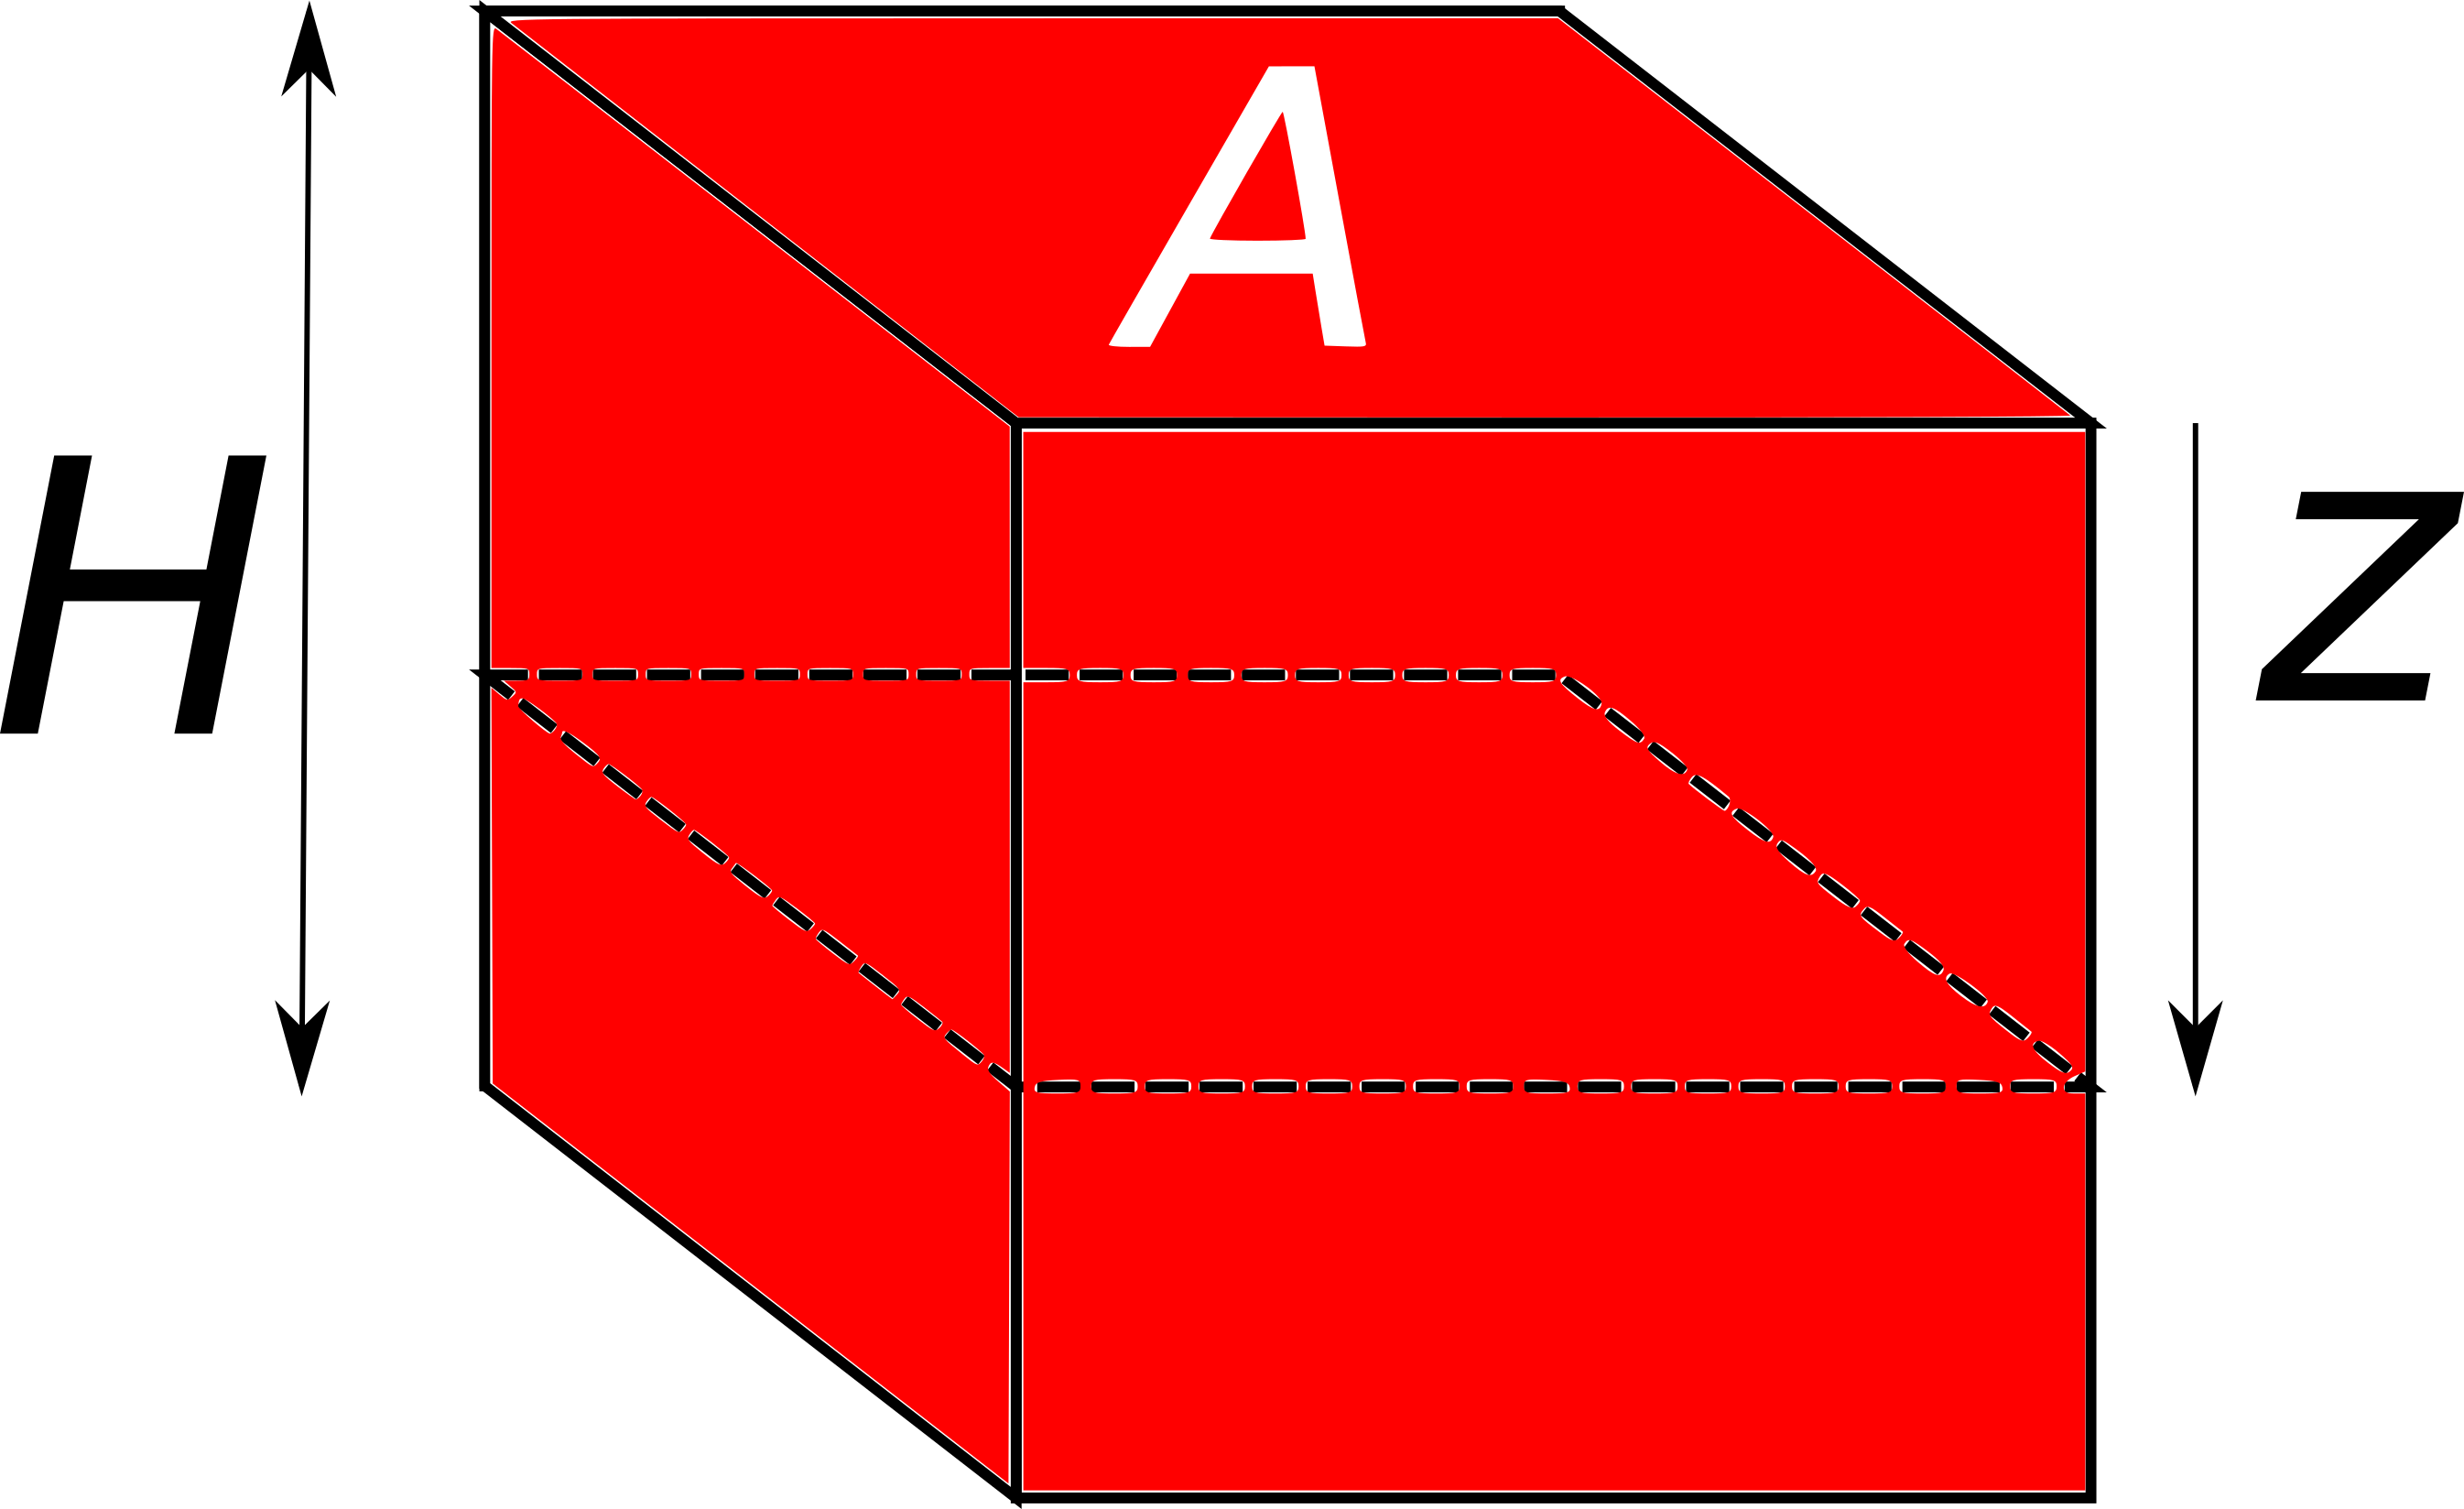
\includegraphics[width=0.8\textwidth]{column_xsec.png}$$
      
    \end{column}

  \end{columns}
  
\end{frame}
%-----------------------------------------------
\begin{frame}
  \frametitle{Hydrostatic gradients}

  \begin{columns}[t]

    \begin{column}{0.5\paperwidth}

      Nothing is moving $\implies$ \textbf{Mechanical equilibrium} \\

      $$ W = F_{\text{p}} $$

      $$ P = \rho g z $$

      $$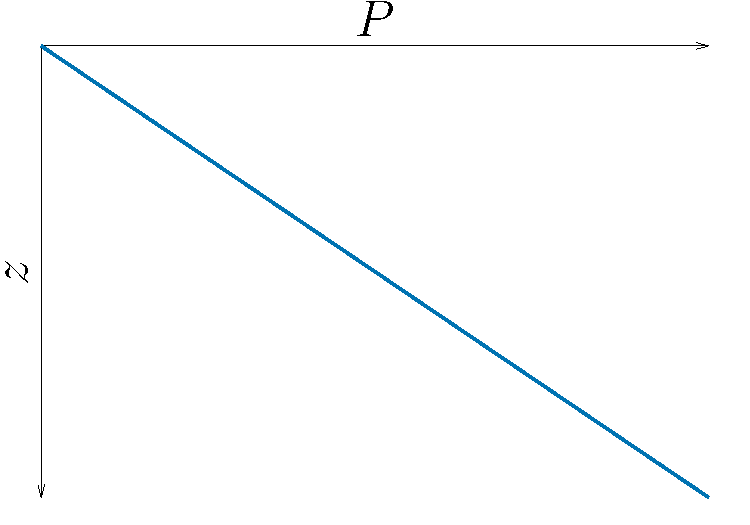
\includegraphics[width=0.8\textwidth]{hydrostat_1fluid.pdf}$$
      
    \end{column}

    \begin{column}{0.49\paperwidth}

      $$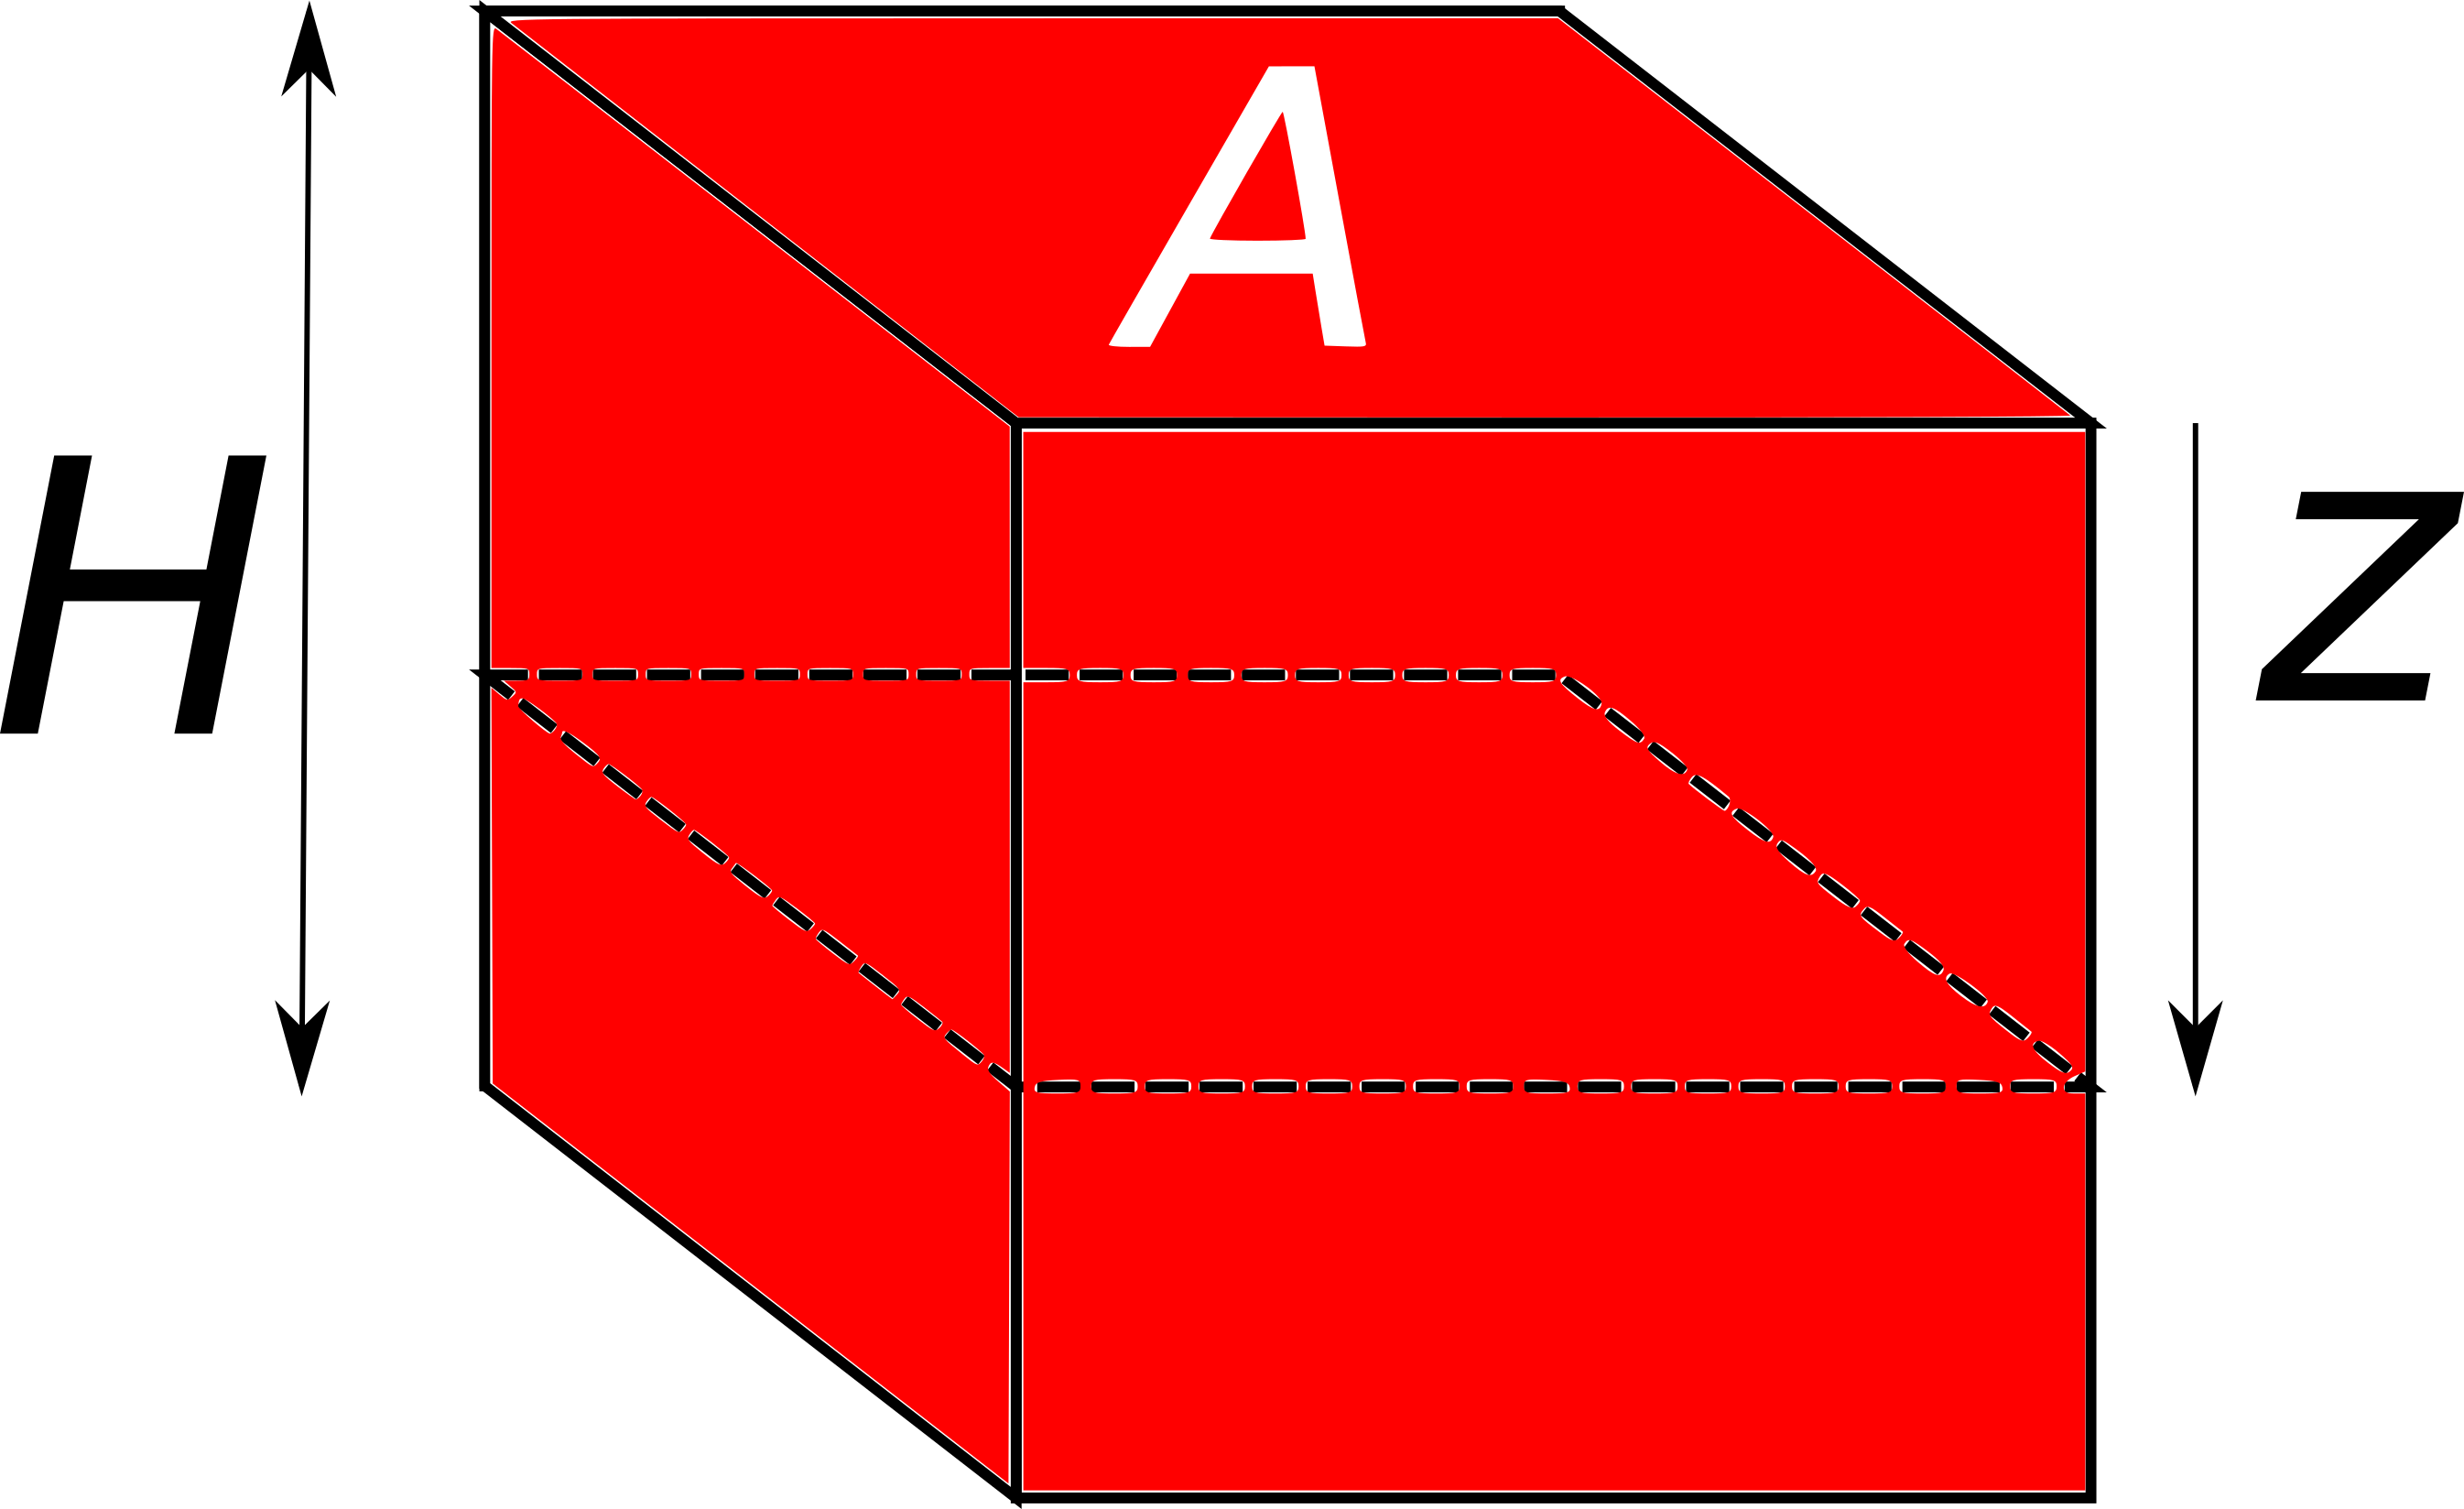
\includegraphics[width=0.8\textwidth]{column_xsec.png}$$

      $P$ increases linearly with $z$ \\

      \vspace{0.5cm}
      
      \textbf{Hydrostatic gradient}:

      $$ \frac{\mathrm{d} P}{\mathrm{d} z} = \rho g $$
    \end{column}

  \end{columns}
  
\end{frame}
%-----------------------------------------------
\begin{frame}
  \frametitle{Gravity currents - Hydrostatic gradients}

  \textbf{Gravity current} - A horizontal flow in a gravitational field that is driven by a density difference \\

  \begin{columns}[t]

    \begin{column}{0.5\paperwidth}

      \vspace{-1cm}
      
      $$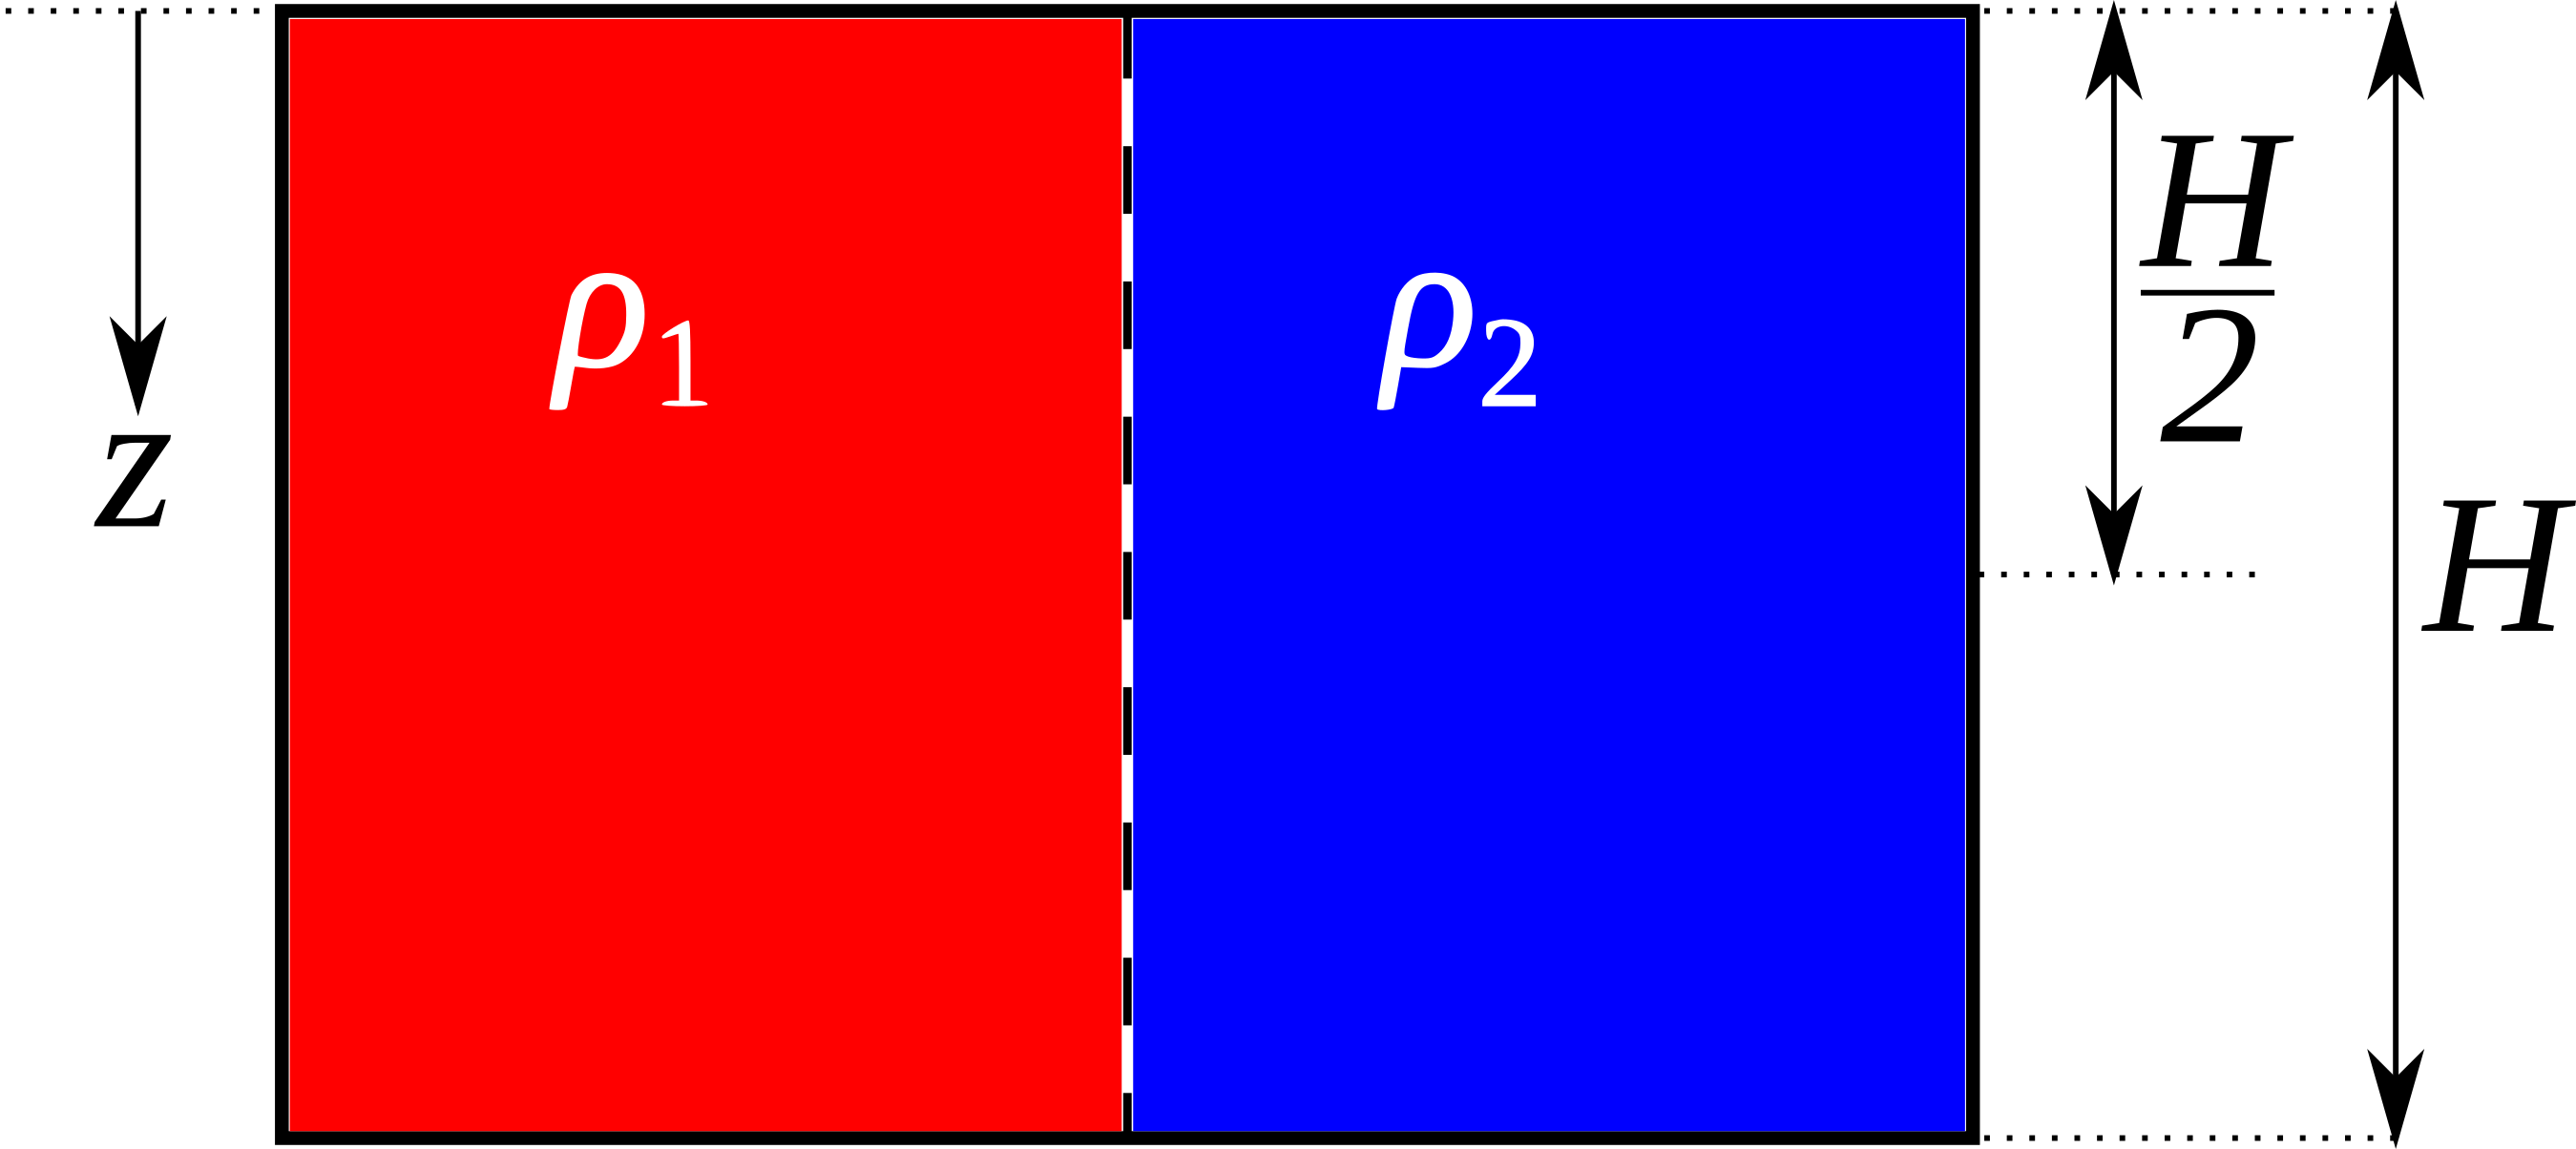
\includegraphics[width=0.8\textwidth]{isostatic.png}$$

      \vspace{-1cm}
      
      $$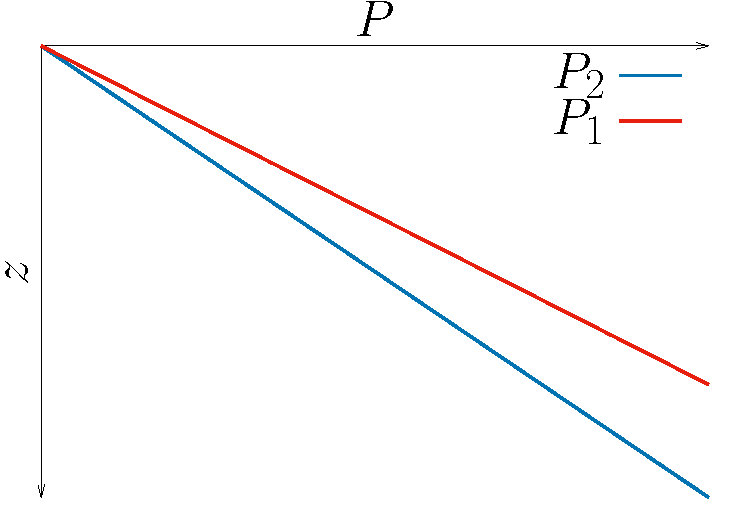
\includegraphics[width=0.8\textwidth]{hydrostat.pdf}$$
      
    \end{column}

    \begin{column}{0.49\paperwidth}

      \vspace{-0.5cm}
      
      Consider two fluids (densities $\rho_{1}$ and $\rho_{2}$, $\rho_{1} > \rho_{2}$) initially side-by-side and separated by a vertical barrier \\

      Vertical pressure gradient:

      $$ \frac{\mathrm{d} P}{\mathrm{d} z} = \rho g$$

      $$ \mathrm{d} P = \rho g \mathrm{d}z $$

      $$ \int_{0}^{P} \mathrm{d} P = \rho g \int_{0}^{z} \mathrm{d} z $$

      $$ P = \rho g z$$
    \end{column}

  \end{columns}
  
\end{frame}
%-----------------------------------------------
\begin{frame}
  \frametitle{Gravity currents - Horizontal force balance}

  \begin{columns}[t]

    \begin{column}{0.5\paperwidth}

      \vspace{-1cm}
      
      $$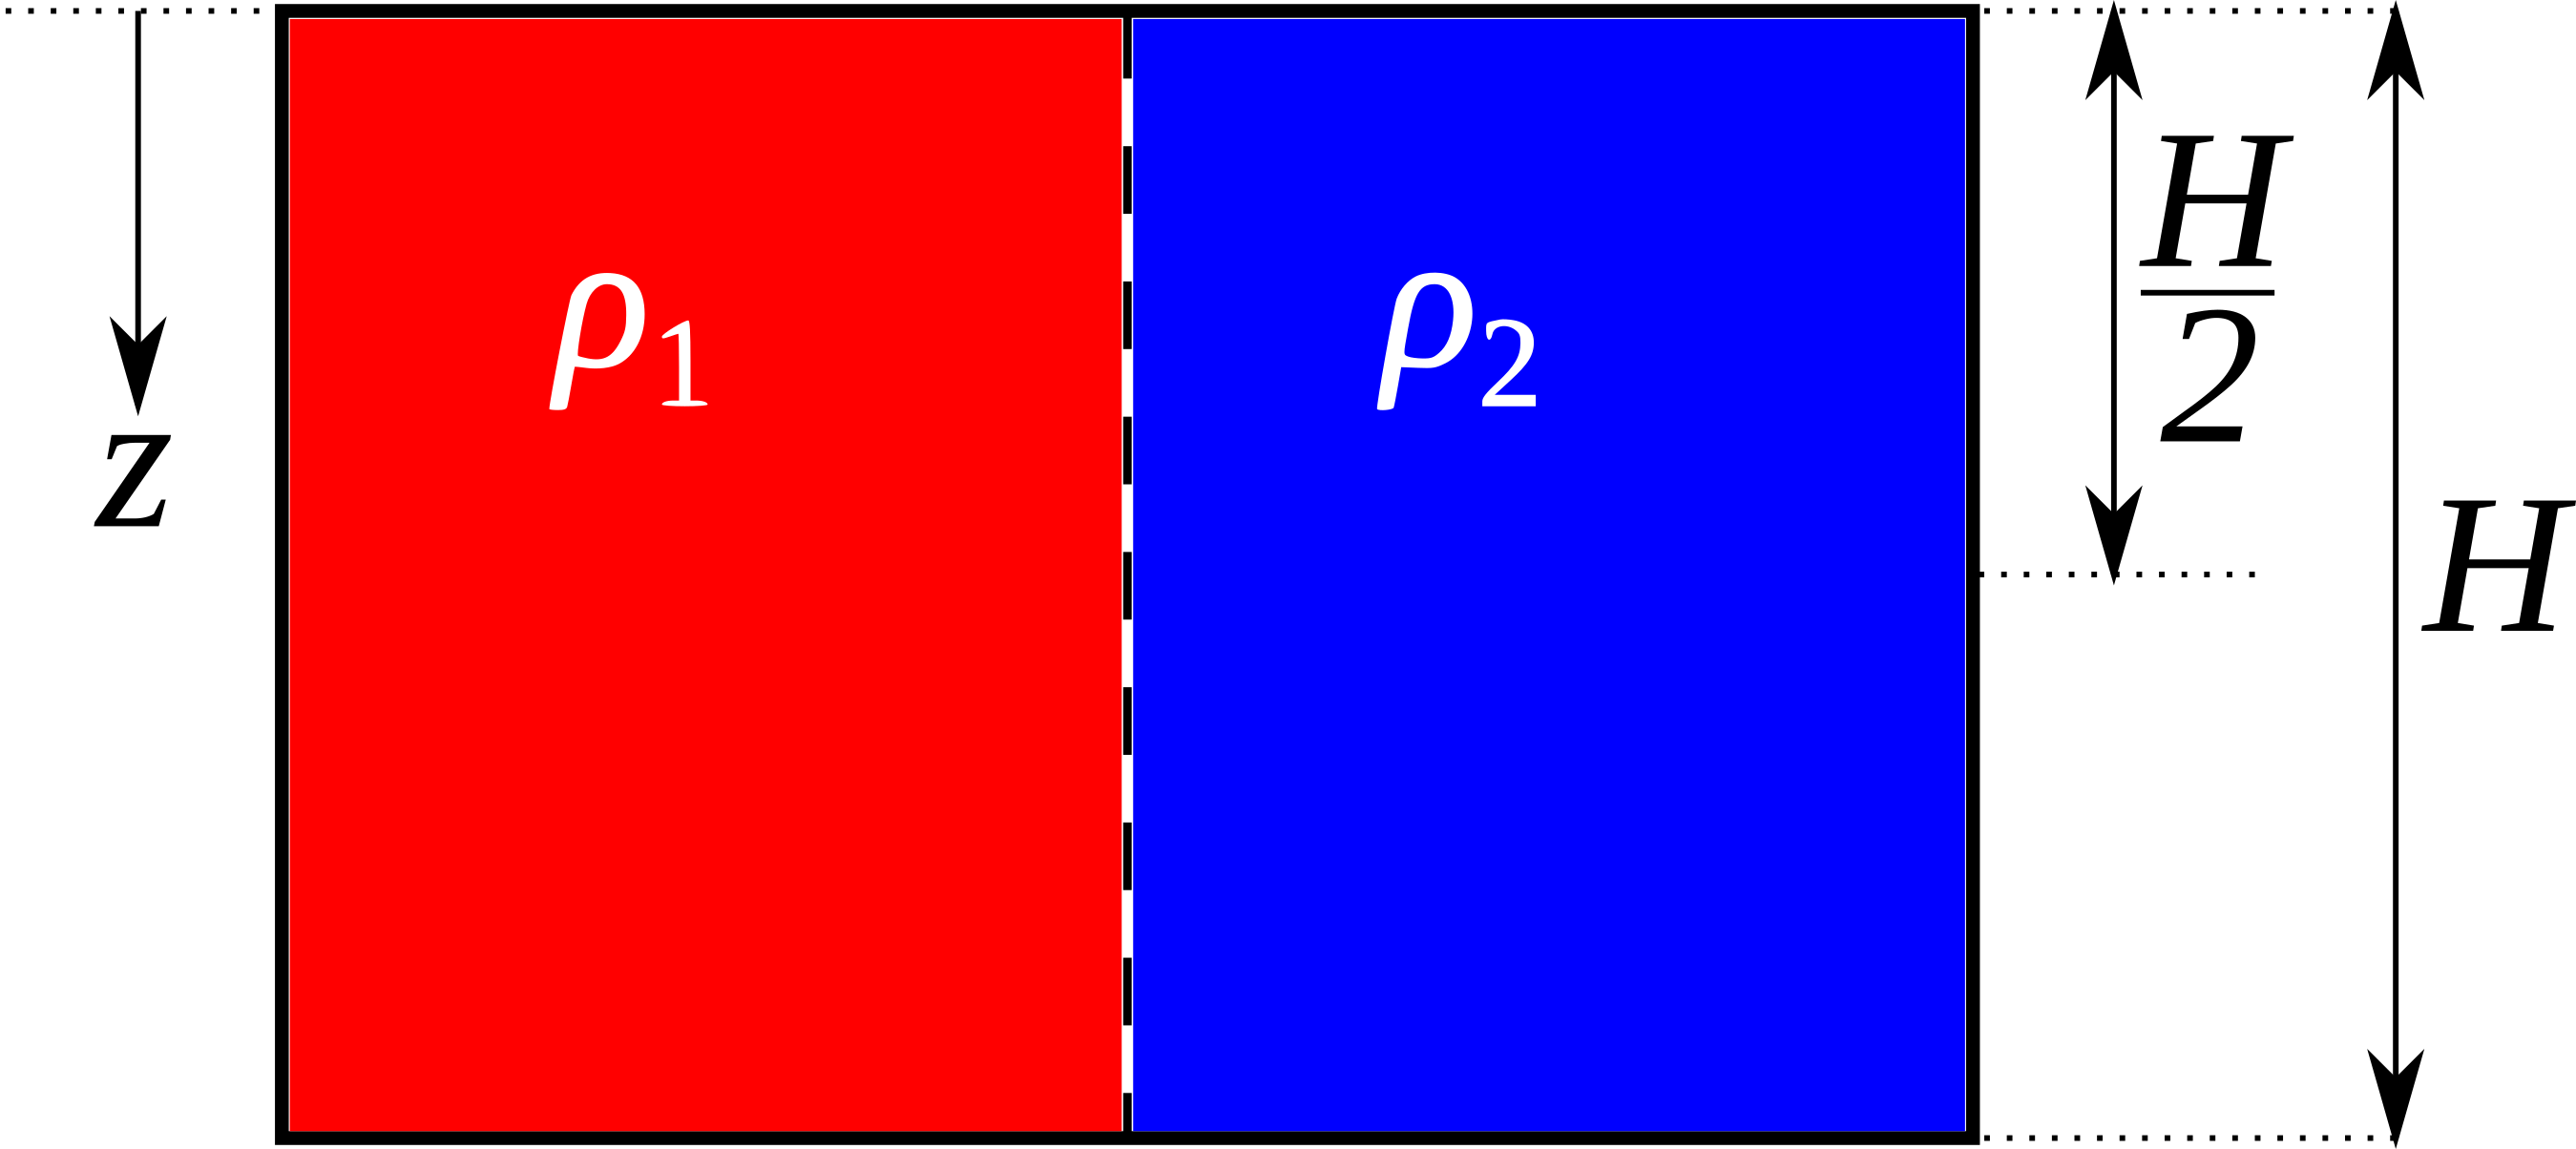
\includegraphics[width=0.8\textwidth]{isostatic.png}$$

      \vspace{-1cm}
      
      $$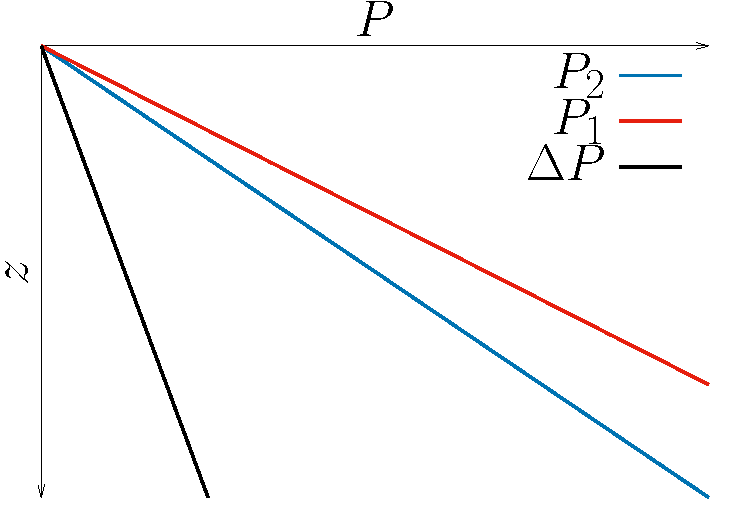
\includegraphics[width=0.8\textwidth]{hydrostat_diff.pdf}$$
      
    \end{column}

    \begin{column}{0.49\paperwidth}

      \vspace{-0.5cm}

      Remove barrier, and consider pressure difference $\Delta P$ across line \\

      \vspace{0.1cm}

      $\Delta P$ increases with depth \\

      \vspace{0.1cm}

      Flow follows a pressure gradient - but horizontal pressure gradient is greatest at the depth \\

      \vspace{0.1cm}

      This initiates from from high to low pressure at the base, which is compensated by return flow at the top \\

      \vspace{-0.5cm}
      
      $$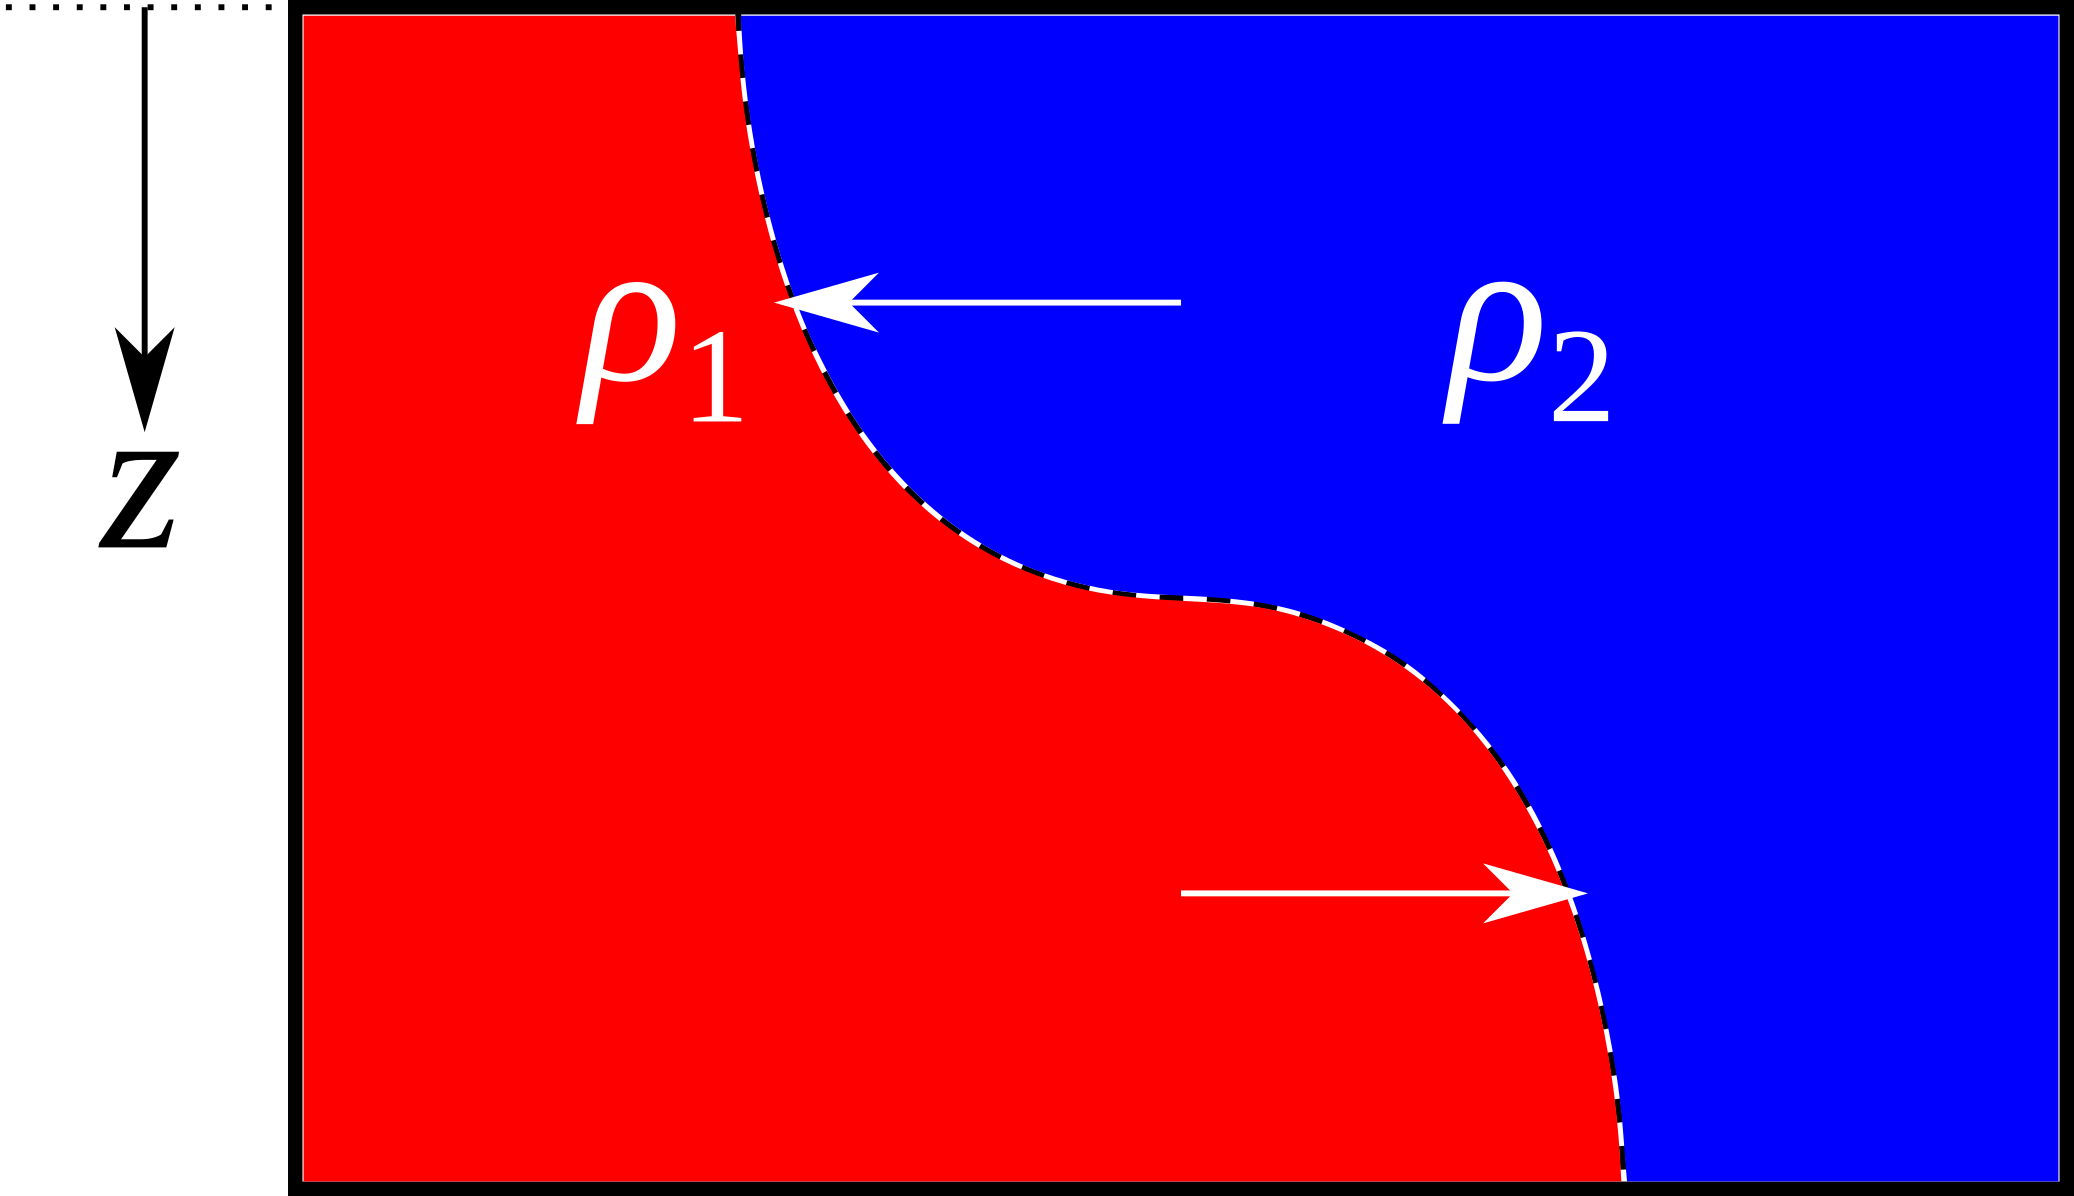
\includegraphics[width=0.8\textwidth]{grav_curr.png}$$
      
    \end{column}

  \end{columns}
  
\end{frame}
%-----------------------------------------------
\begin{frame}
  \frametitle{Gravitational potential energy (GPE)}

  \begin{columns}[t]

    \begin{column}{0.5\paperwidth}

      $$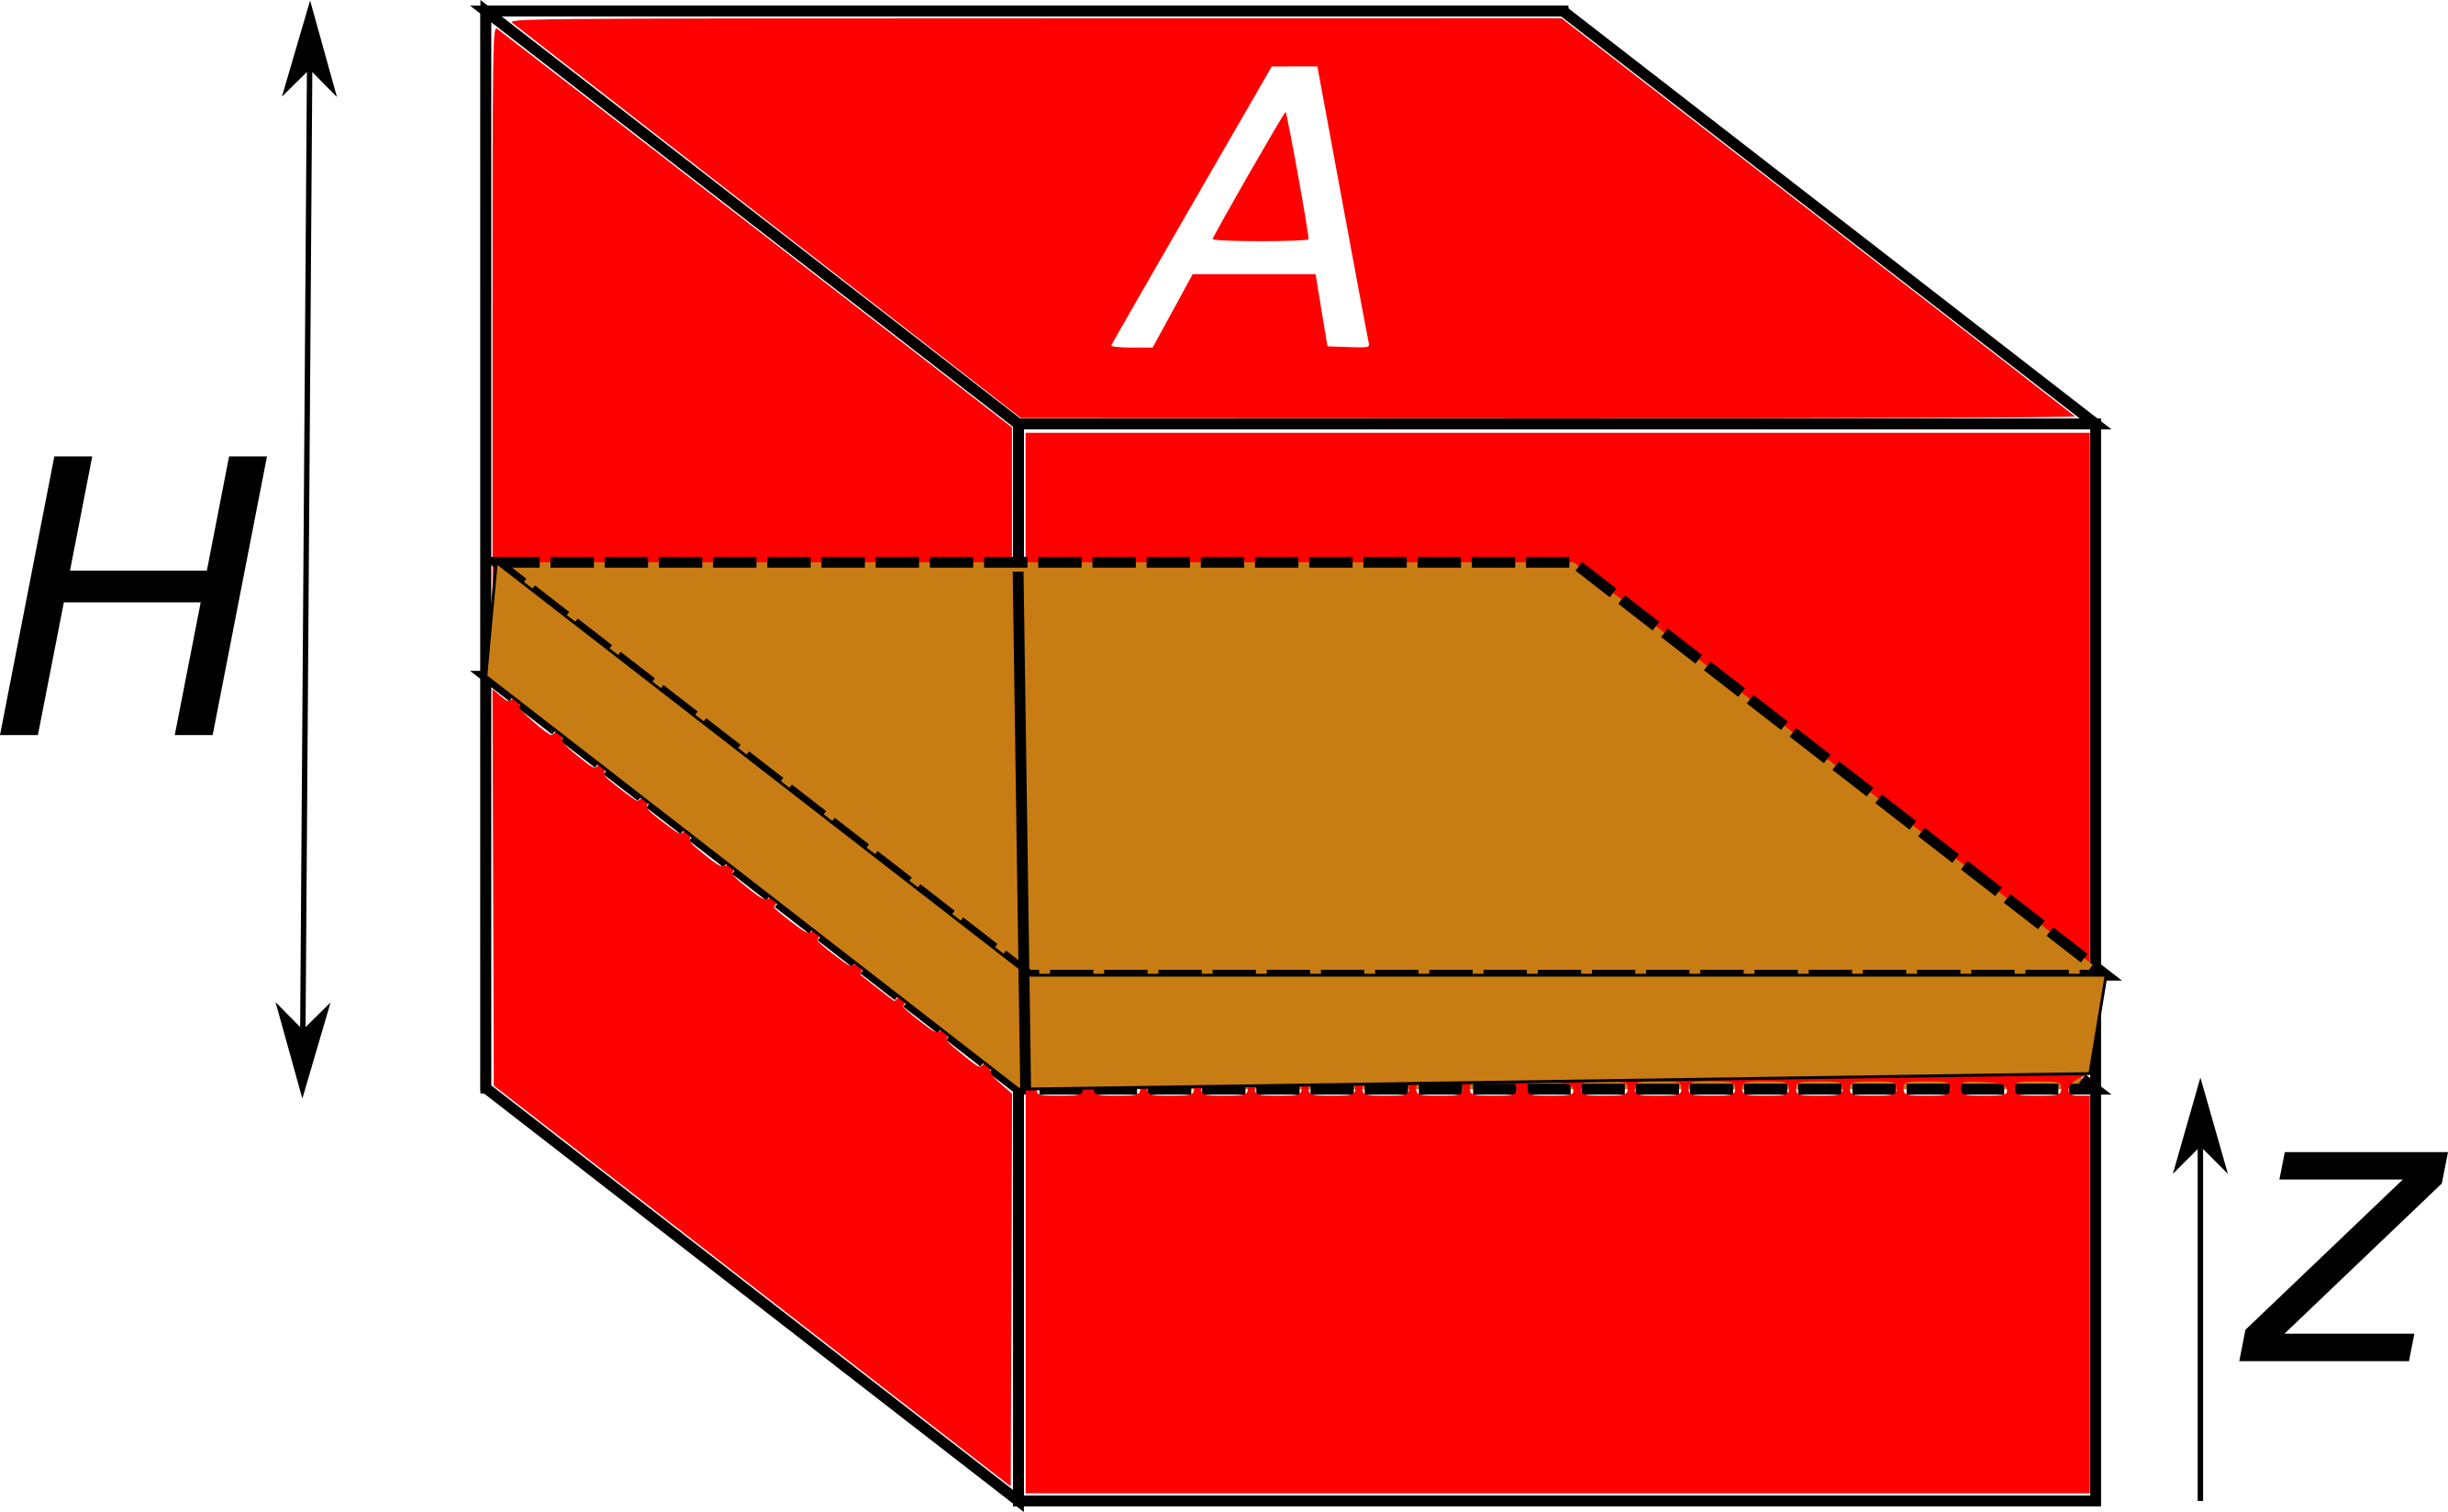
\includegraphics[width=0.8\textwidth]{column_energy.png}$$
      
    \end{column}

    \begin{column}{0.49\paperwidth}

      GPE of thin layer:

      $$\mathrm{d} U = \rho A \mathrm{d}z  g z = \rho g A z \mathrm{d} z$$ \\

      GPE of total column:

      $$U = \int_{z = 0}^{H} \mathrm{d}U  $$

      $$ U = \rho g A \int_{z = 0}^{H} z \mathrm{d} z $$

      $$ U = \rho g A \left[ \frac{z}{2} \right]_{z = 0}^{H} $$

      $$ U = \frac{\rho g A H^{2}}{2} $$
    \end{column}

  \end{columns}

  
\end{frame}
%-----------------------------------------------
\begin{frame}
  \frametitle{Gravity currents - Energy minimisation}

  Initial state:
  
  \begin{columns}[t]

    \begin{column}{0.45\paperwidth}

      $$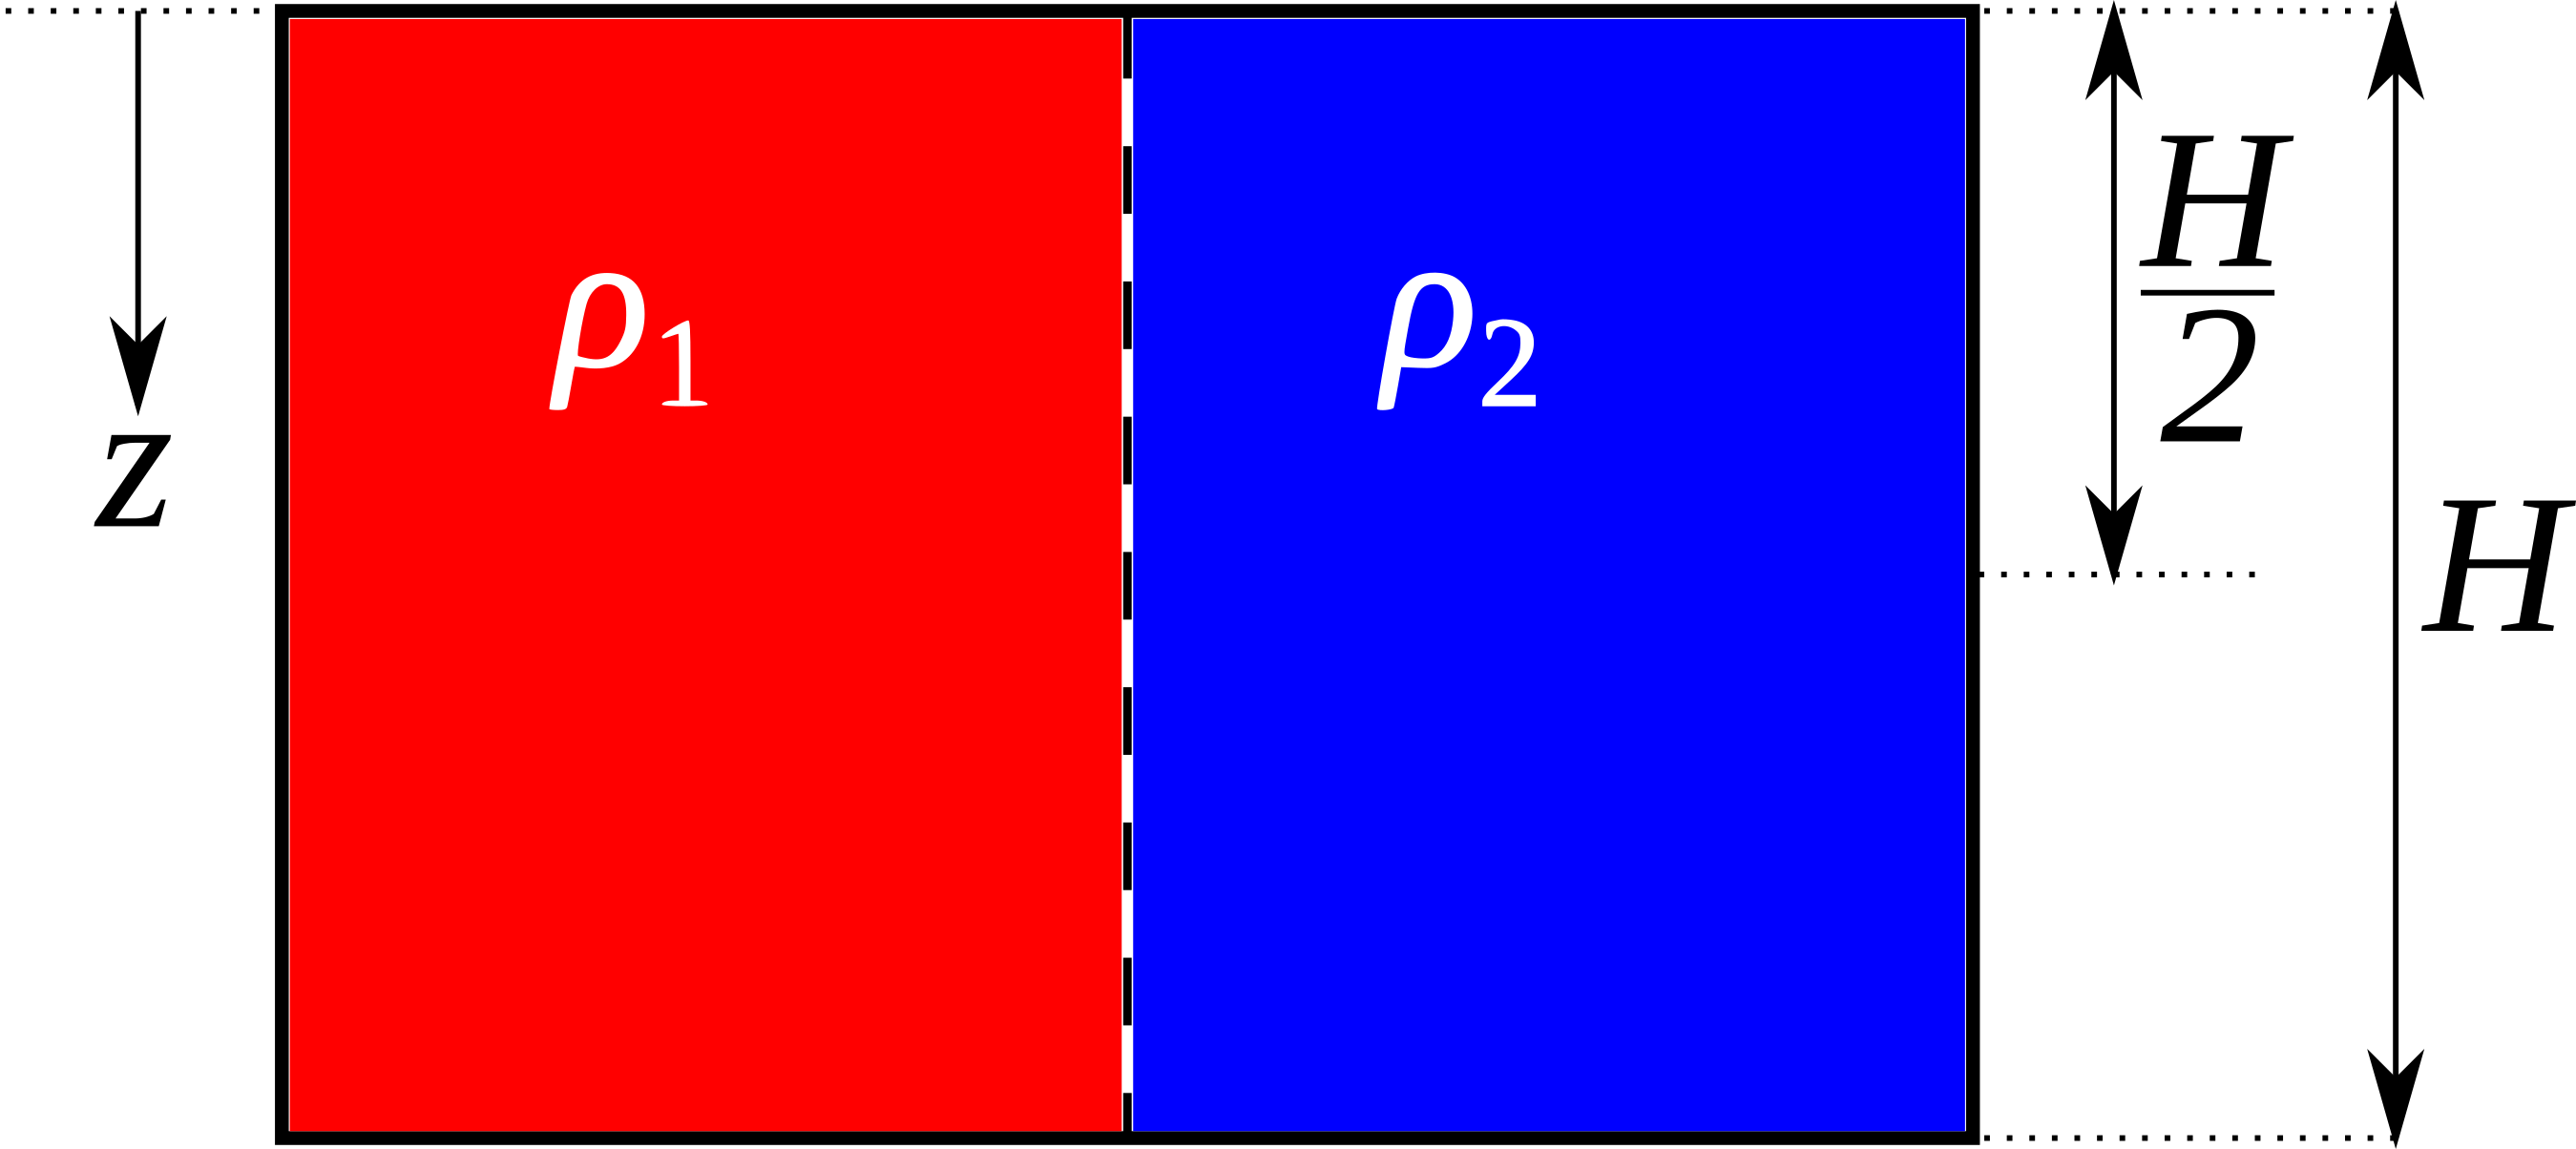
\includegraphics[width=0.9\textwidth]{isostatic.png}$$
      
    \end{column}

    \begin{column}{0.55\paperwidth}

      \vspace{-1cm}

      GPE of thin layer:

      $$\mathrm{d} U = \frac{(\rho_{1} + \rho_{2}) A \mathrm{d}z  g z}{2} = \frac{(\rho_{1} + \rho_{2}) g A z \mathrm{d} z}{2}$$ \\

      GPE of total column:

      $$U_{i} = \int_{z = 0}^{H} \mathrm{d}U  $$

      $$ U_{i} = \frac{(\rho_{1} + \rho_{2}) g A}{2} \int_{z = 0}^{H} z \mathrm{d} z $$

      $$ U_{i} = \frac{(\rho_{1} + \rho_{2}) g A}{2} \left[ \frac{z}{2} \right]_{z = 0}^{H} $$

      $$ U_{i} = \frac{(\rho_{1} + \rho_{2}) g A H^{2}}{4} $$
      
    \end{column}

  \end{columns}

  
\end{frame}
%-----------------------------------------------
\begin{frame}
  \frametitle{Gravity currents - Energy minimisation}

  Final state:
  
  \begin{columns}[t]

    \begin{column}{0.4\paperwidth}

      $$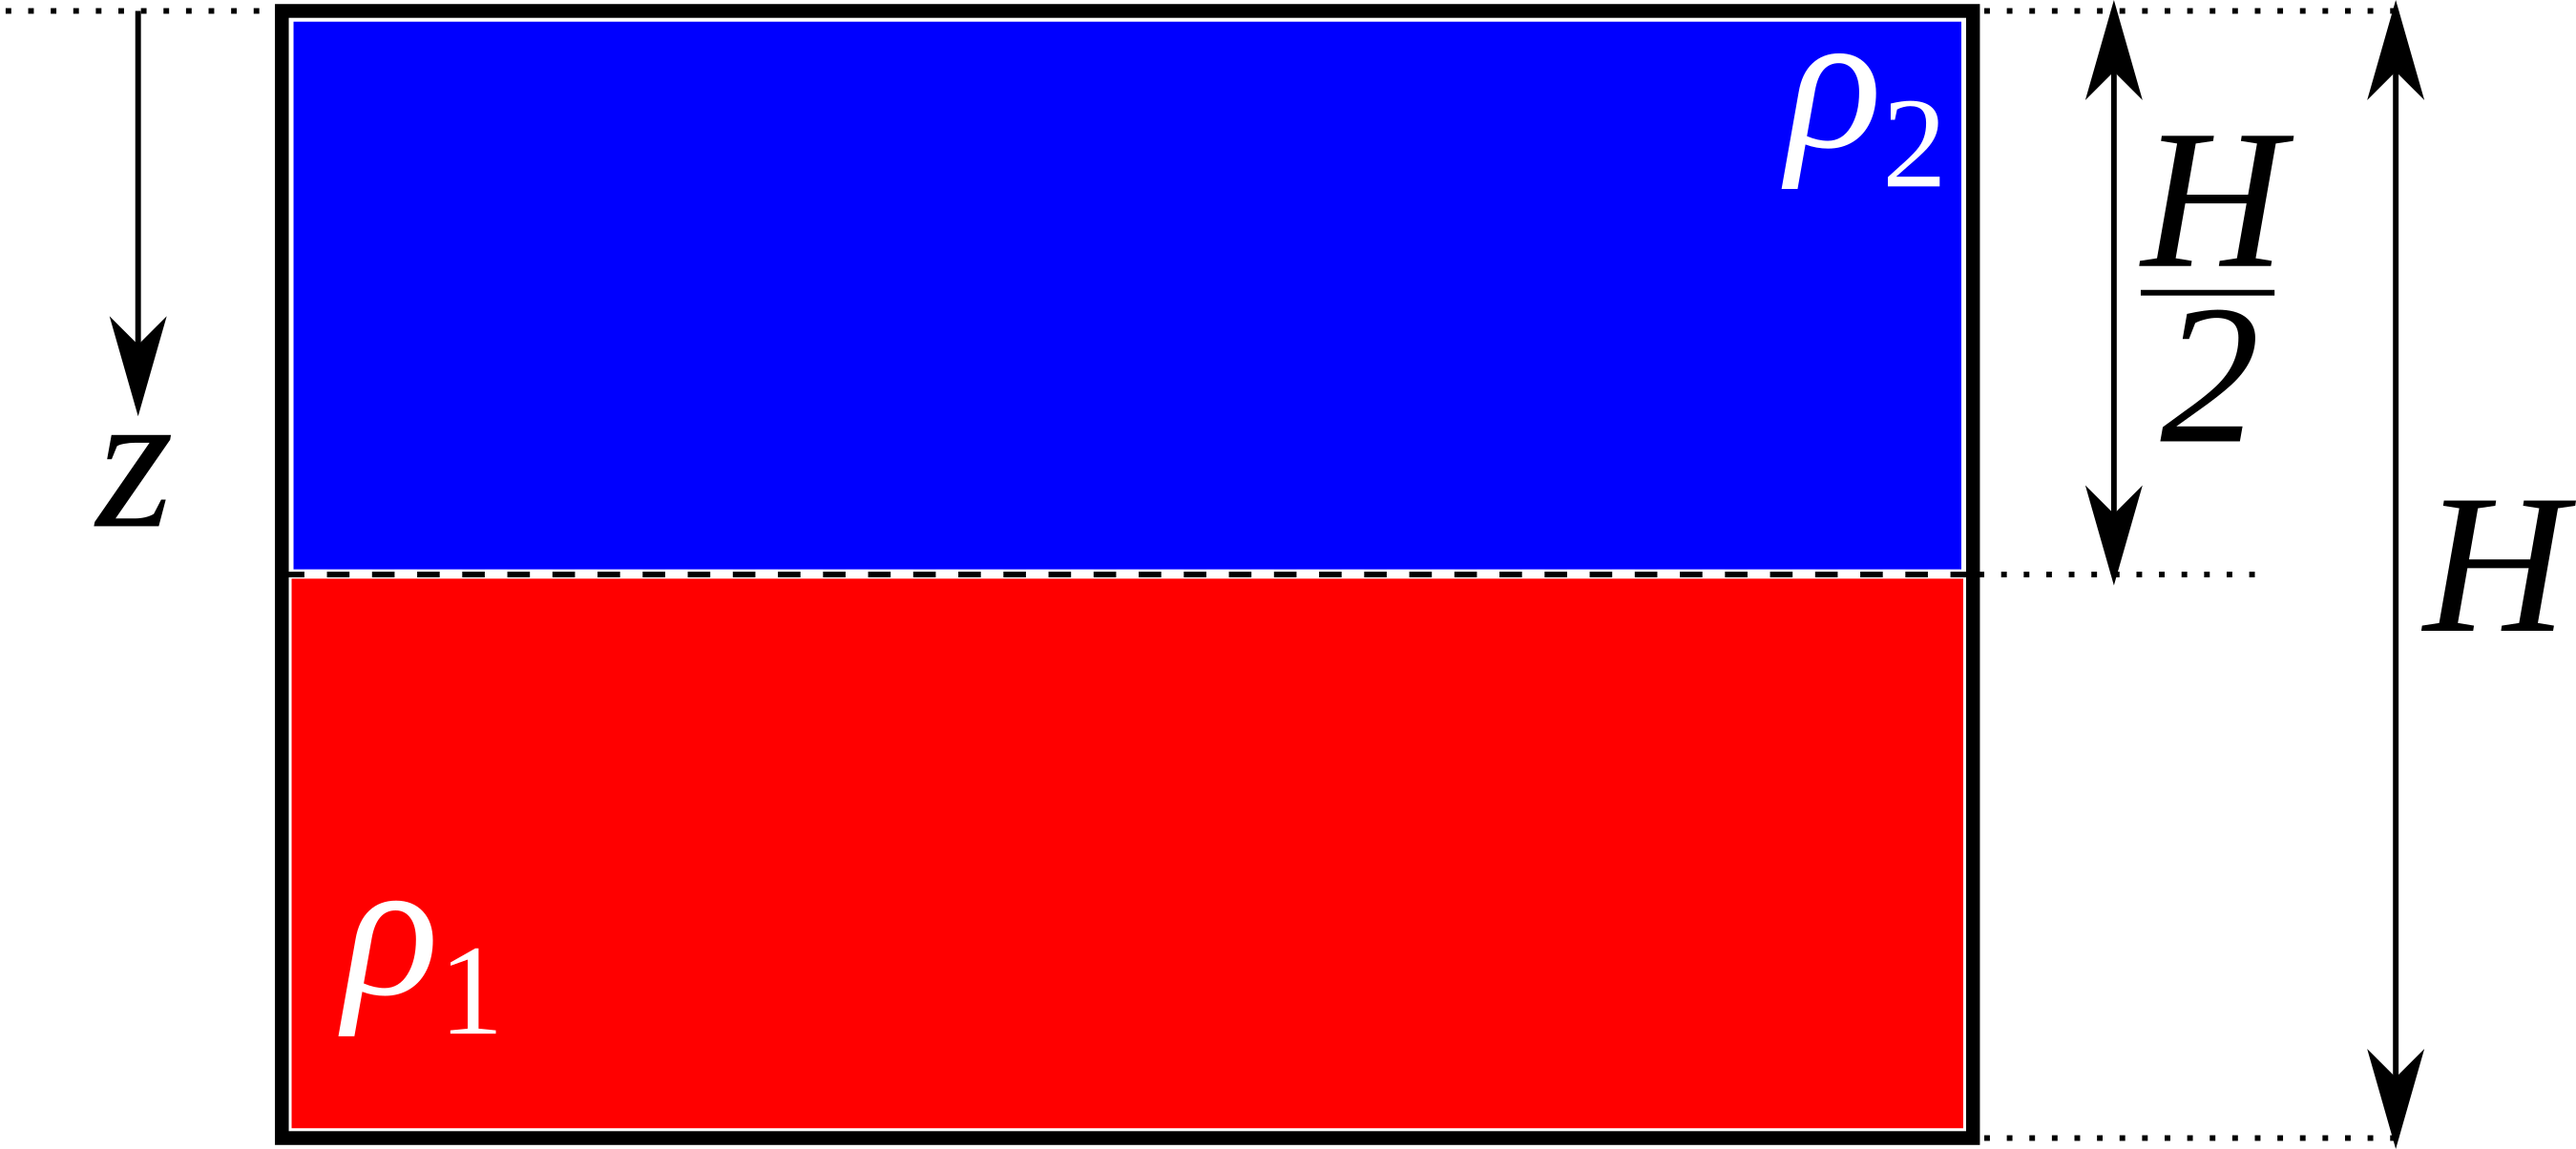
\includegraphics[width=\textwidth]{stratified.png}$$
      
    \end{column}

    \begin{column}{0.6\paperwidth}

      \vspace{-1cm}

      $$ U_{f} = g A \left( \rho_{1} \int_{z = 0}^{H / 2} z \mathrm{d} z + \rho_{2} \int_{z = H / 2}^{H} z \mathrm{d} z \right)$$

      $$ U_{f} = g A \left(\rho_{1} \left[ \frac{z^{2}}{2} \right]_{z = 0}^{H / 2} + \rho_{2} \left[ \frac{z^{2}}{2} \right]_{z = H / 2}^{H} \right) $$

      $$ U_{f} = \frac{g A}{2} \left[ \frac{\rho_{1} H^{2}}{4} + \rho_{2} \left(H^{2} - \frac{H^{2}}{4} \right) \right] $$

      $$ U_{f} = \frac{g A H^{2}}{2} \left( \frac{\rho_{1}}{4} + \frac{3 \rho_{2}}{4} \right) = \frac{g A H^{2} (\rho_{1} + 3 \rho_{2})}{8} $$ 
    \end{column}

  \end{columns}

\end{frame}
%-----------------------------------------------
\begin{frame}
  \frametitle{Gravity currents - Energy minimisation}

  \vspace{-0.5cm}
  
  \begin{columns}[t]

    \begin{column}{0.5\paperwidth}

      \centering Initial state

      \vspace{-0.5cm}

      $$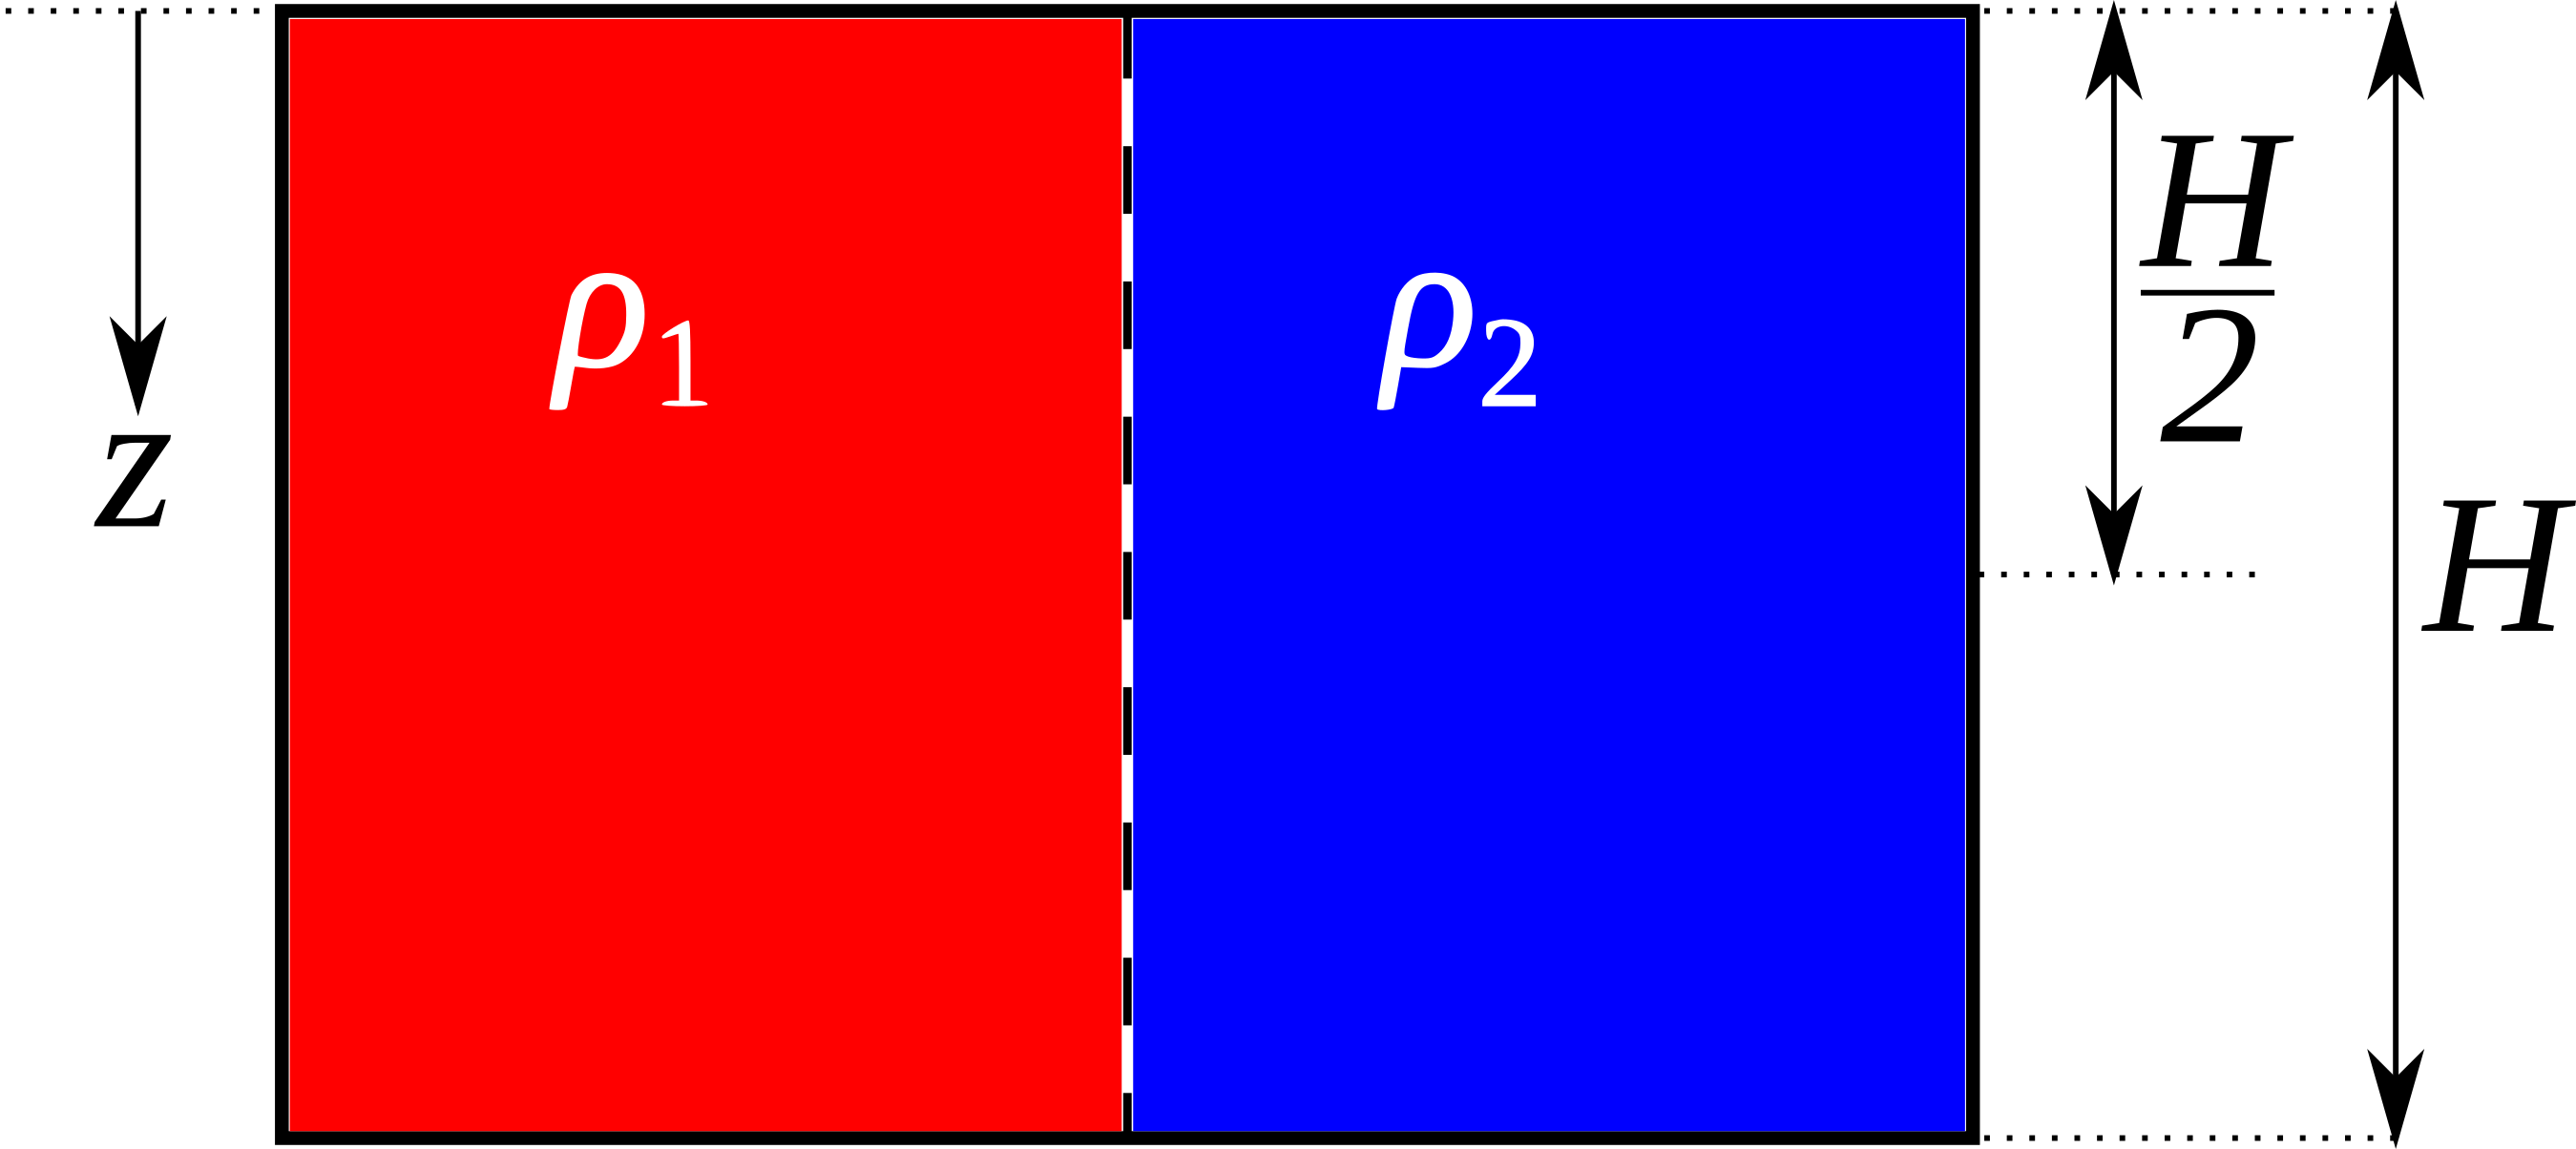
\includegraphics[width=0.9\textwidth]{isostatic.png}$$
      
      \vspace{-0.5cm}

      $$ U_{i} = \frac{(\rho_{1} + \rho_{2}) g A H^{2}}{4} $$
      
    \end{column}

    \begin{column}{0.5\paperwidth}

      \centering Final state

      \vspace{-0.5cm}

      $$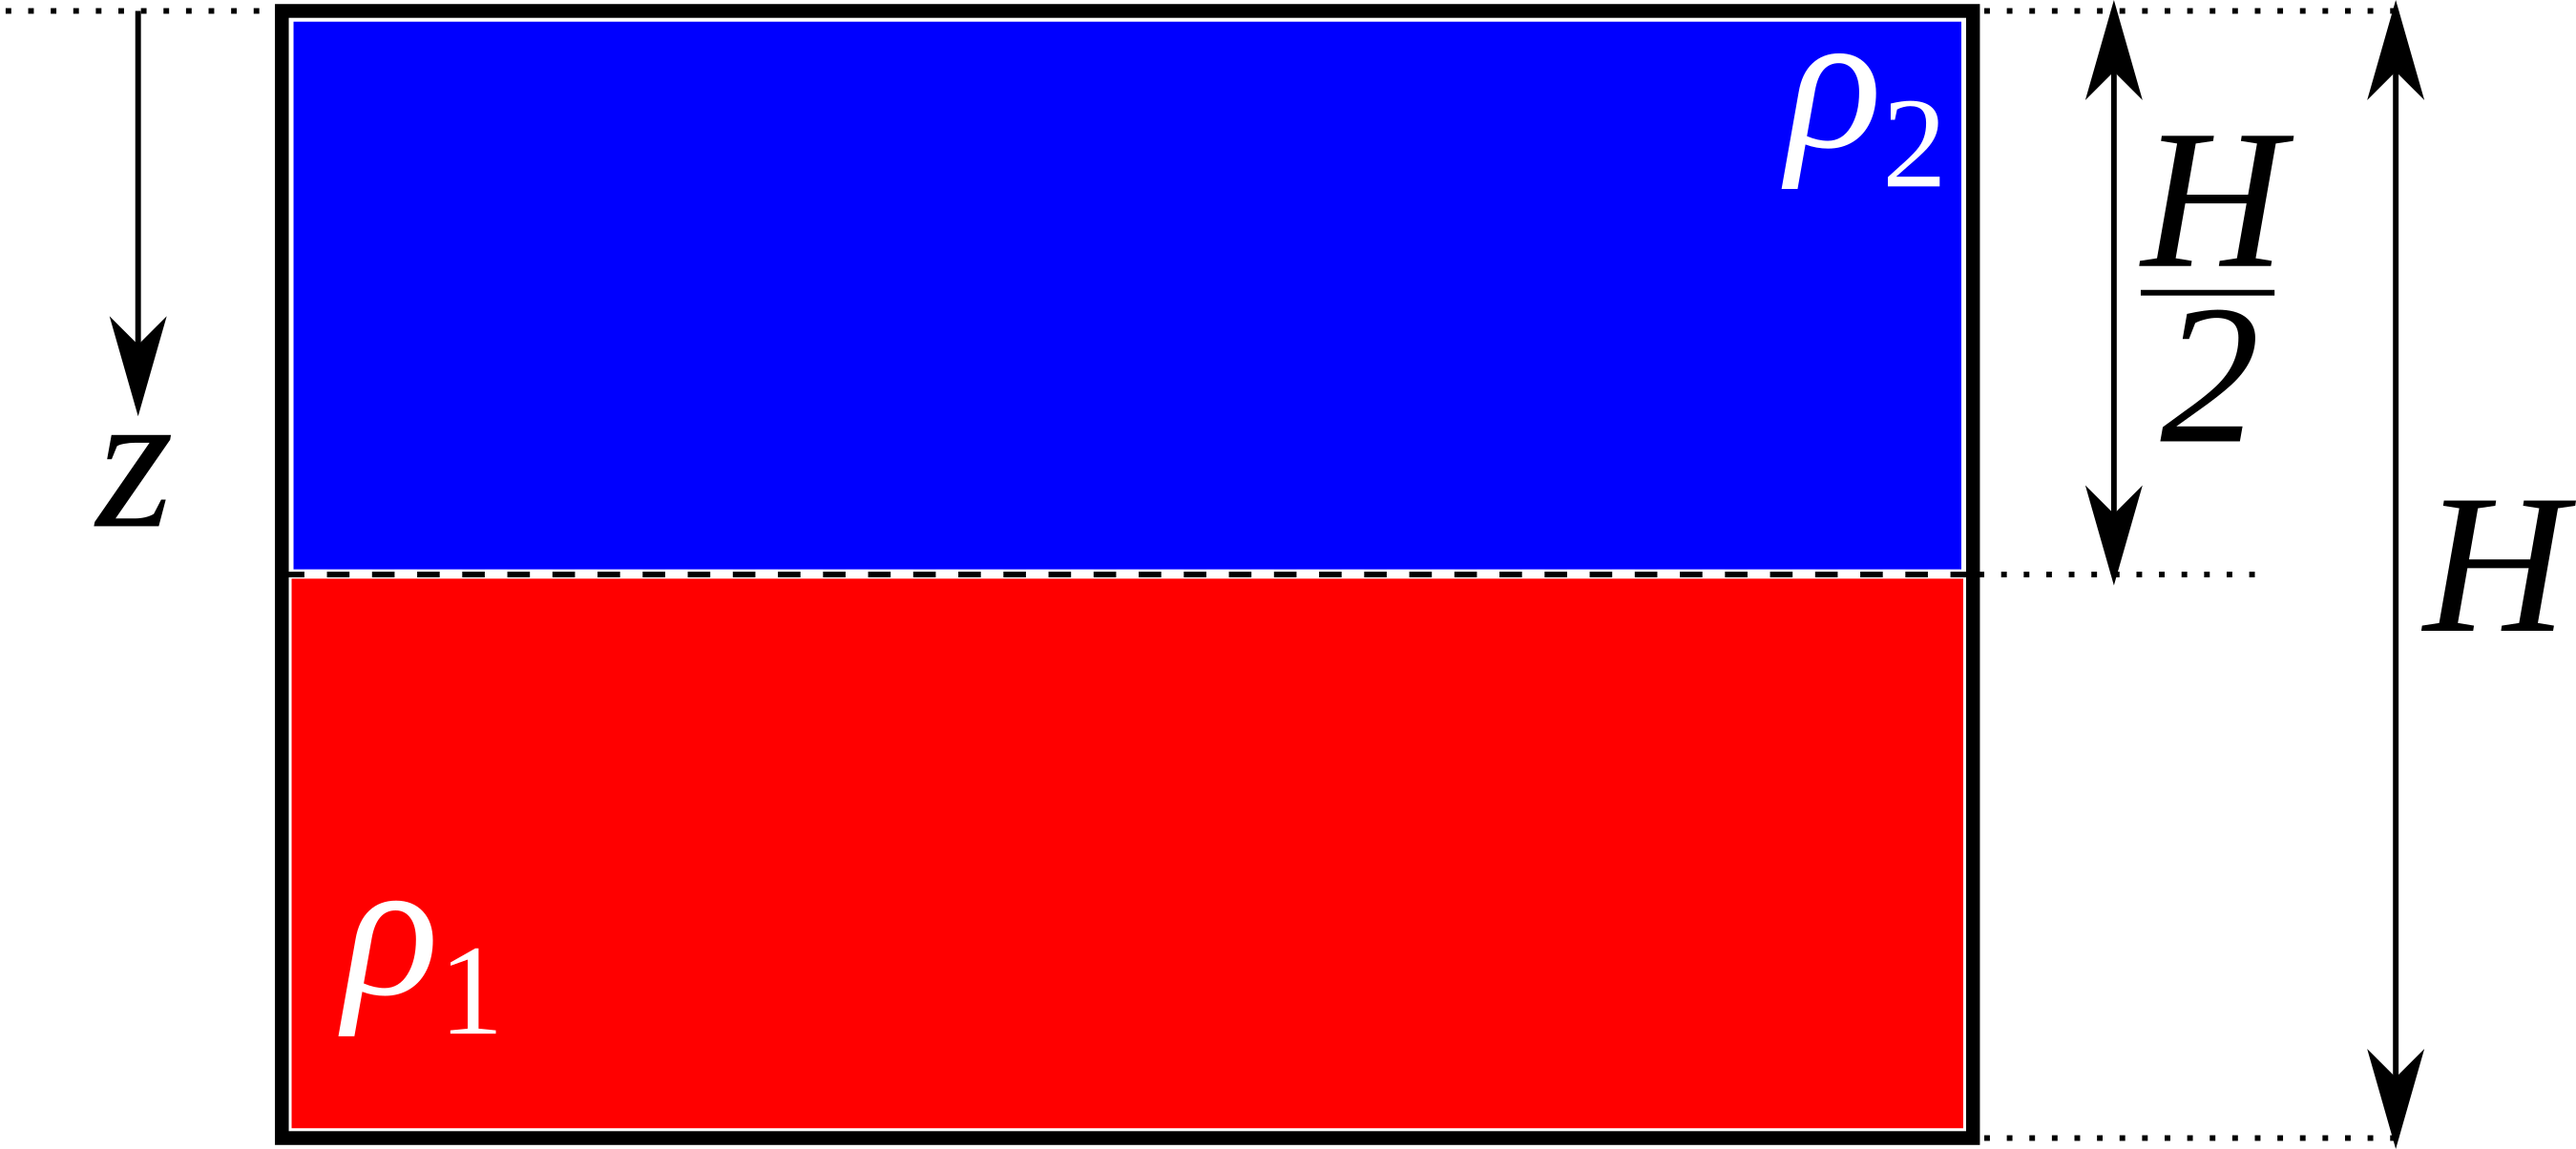
\includegraphics[width=0.9\textwidth]{stratified.png}$$
      
      \vspace{-0.5cm}

      $$ U_{f} = \frac{g A H^{2} (\rho_{1} + 3 \rho_{2})}{8} $$ 
    \end{column}

  \end{columns}

  \vspace{0.5cm}

  $$ U_{f} - U_{i} = \frac{g A H^{2}}{4} \left(\frac{\rho_{1}}{2} + \frac{3 \rho_{2}}{2} - \rho_{1} - \rho_{2} \right) $$

  $$ U_{f} - U_{i} = \frac{g A H^{2}}{4} \left( \frac{\rho_{2} - \rho_{1}}{2} \right) = \frac{g A H^{2} (\rho_{2} - \rho_{1})}{8} $$
\end{frame}
%-----------------------------------------------
\begin{frame}
  \frametitle{Gravity currents - Energy minimisation}

  \vspace{-0.5cm}
  
  \begin{columns}[t]

    \begin{column}{0.5\paperwidth}

      \centering Initial state

      \vspace{-0.5cm}

      $$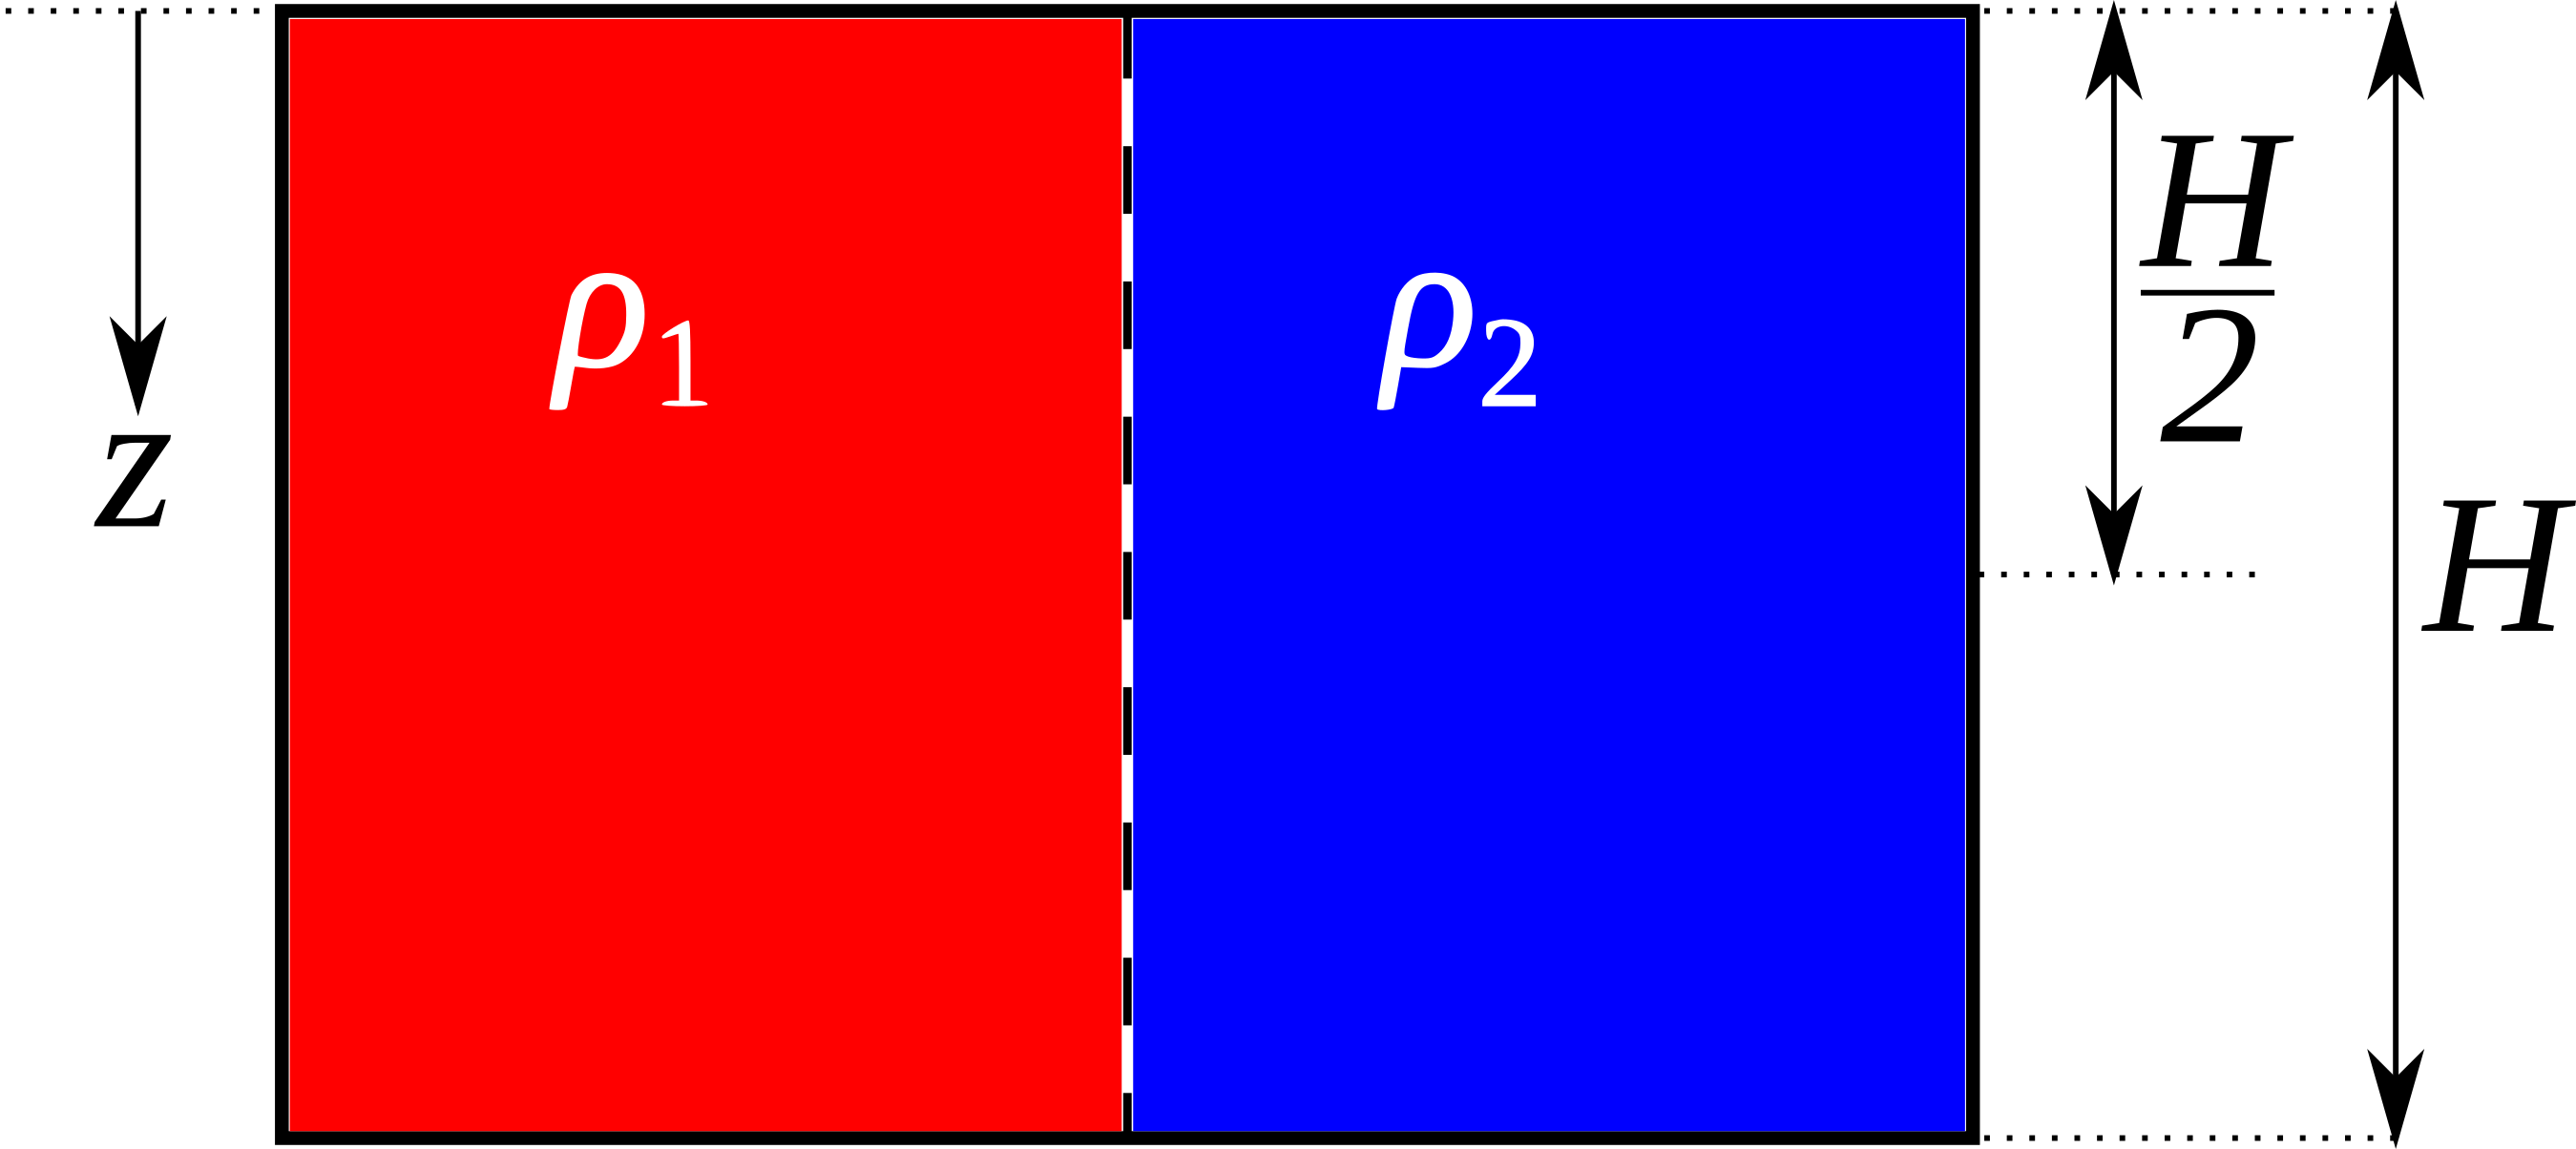
\includegraphics[width=0.9\textwidth]{isostatic.png}$$
      
      \vspace{-0.5cm}

      $$ U_{i} = \frac{(\rho_{1} + \rho_{2}) g A H^{2}}{4} $$
      
    \end{column}

    \begin{column}{0.5\paperwidth}

      \centering Final state

      \vspace{-0.5cm}

      $$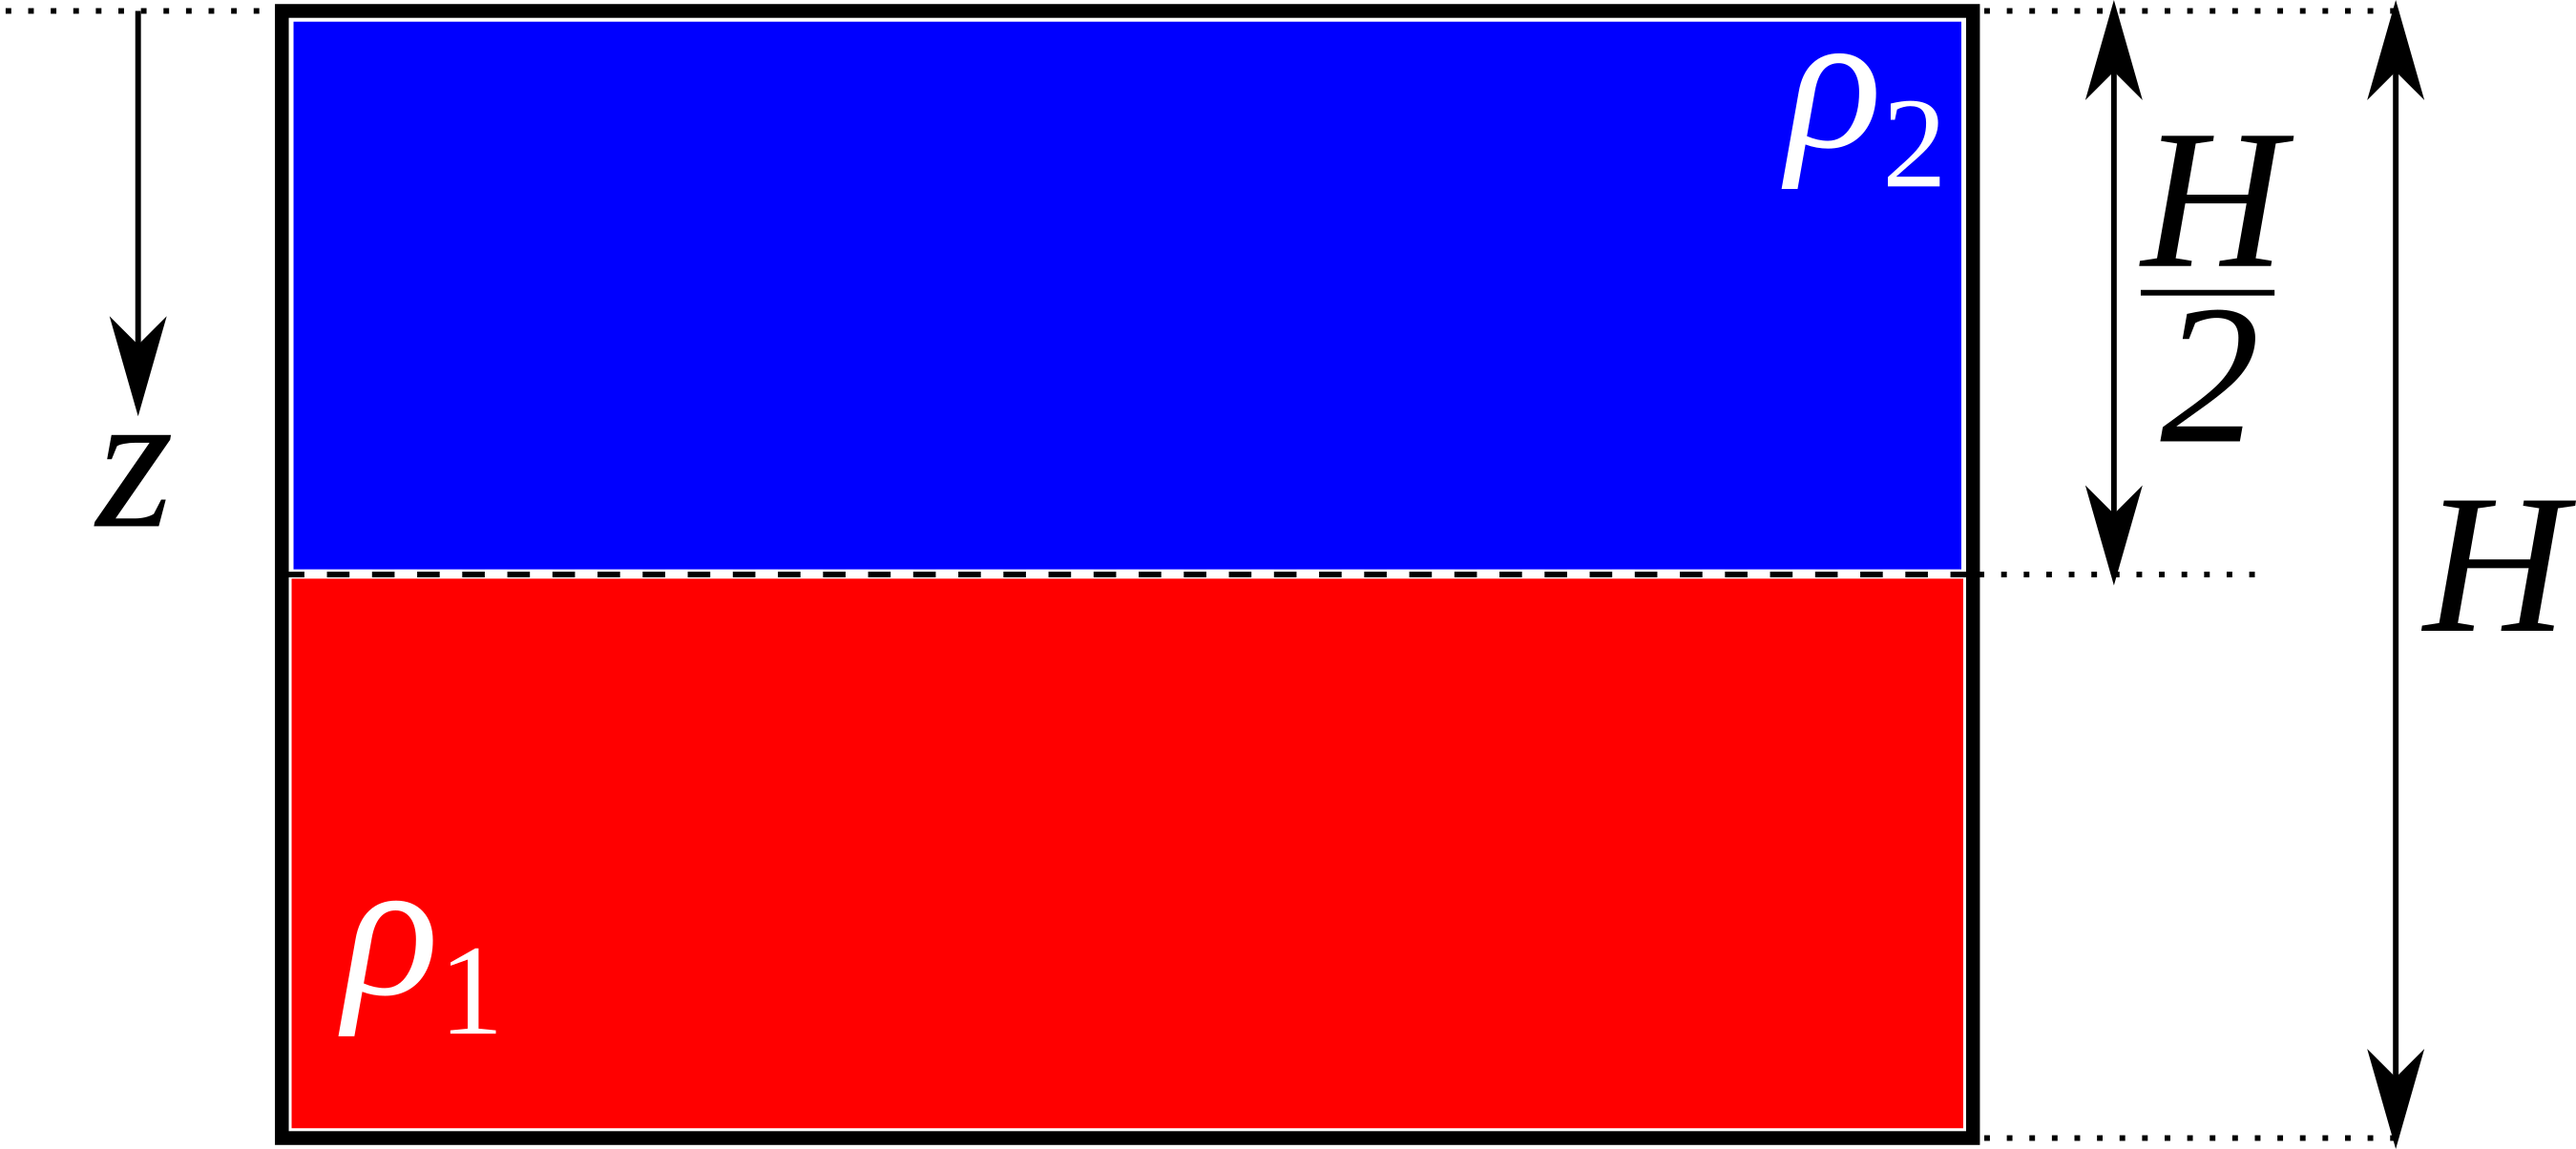
\includegraphics[width=0.9\textwidth]{stratified.png}$$
      
      \vspace{-0.5cm}

      $$ U_{f} = \frac{g A H^{2} (\rho_{1} + 3 \rho_{2})}{8} $$ 
    \end{column}

  \end{columns}

  \vspace{0.5cm}

  $$ U_{f} - U_{i} = \frac{g A H^{2}}{4} \left(\frac{\rho_{1}}{2} + \frac{3 \rho_{2}}{2} - \rho_{1} - \rho_{2} \right) $$

  $$ U_{f} - U_{i} = \frac{g A H^{2}}{4} \left( \frac{\rho_{2} - \rho_{1}}{2} \right) = \frac{g A H^{2} (\rho_{2} - \rho_{1})}{8} $$
\end{frame}
%-----------------------------------------------
\begin{frame}
  \frametitle{Gravity currents - Box models}

  \begin{columns}[t]

    \begin{column}{0.4\paperwidth}

      \vspace{-0.5cm}
      
      $$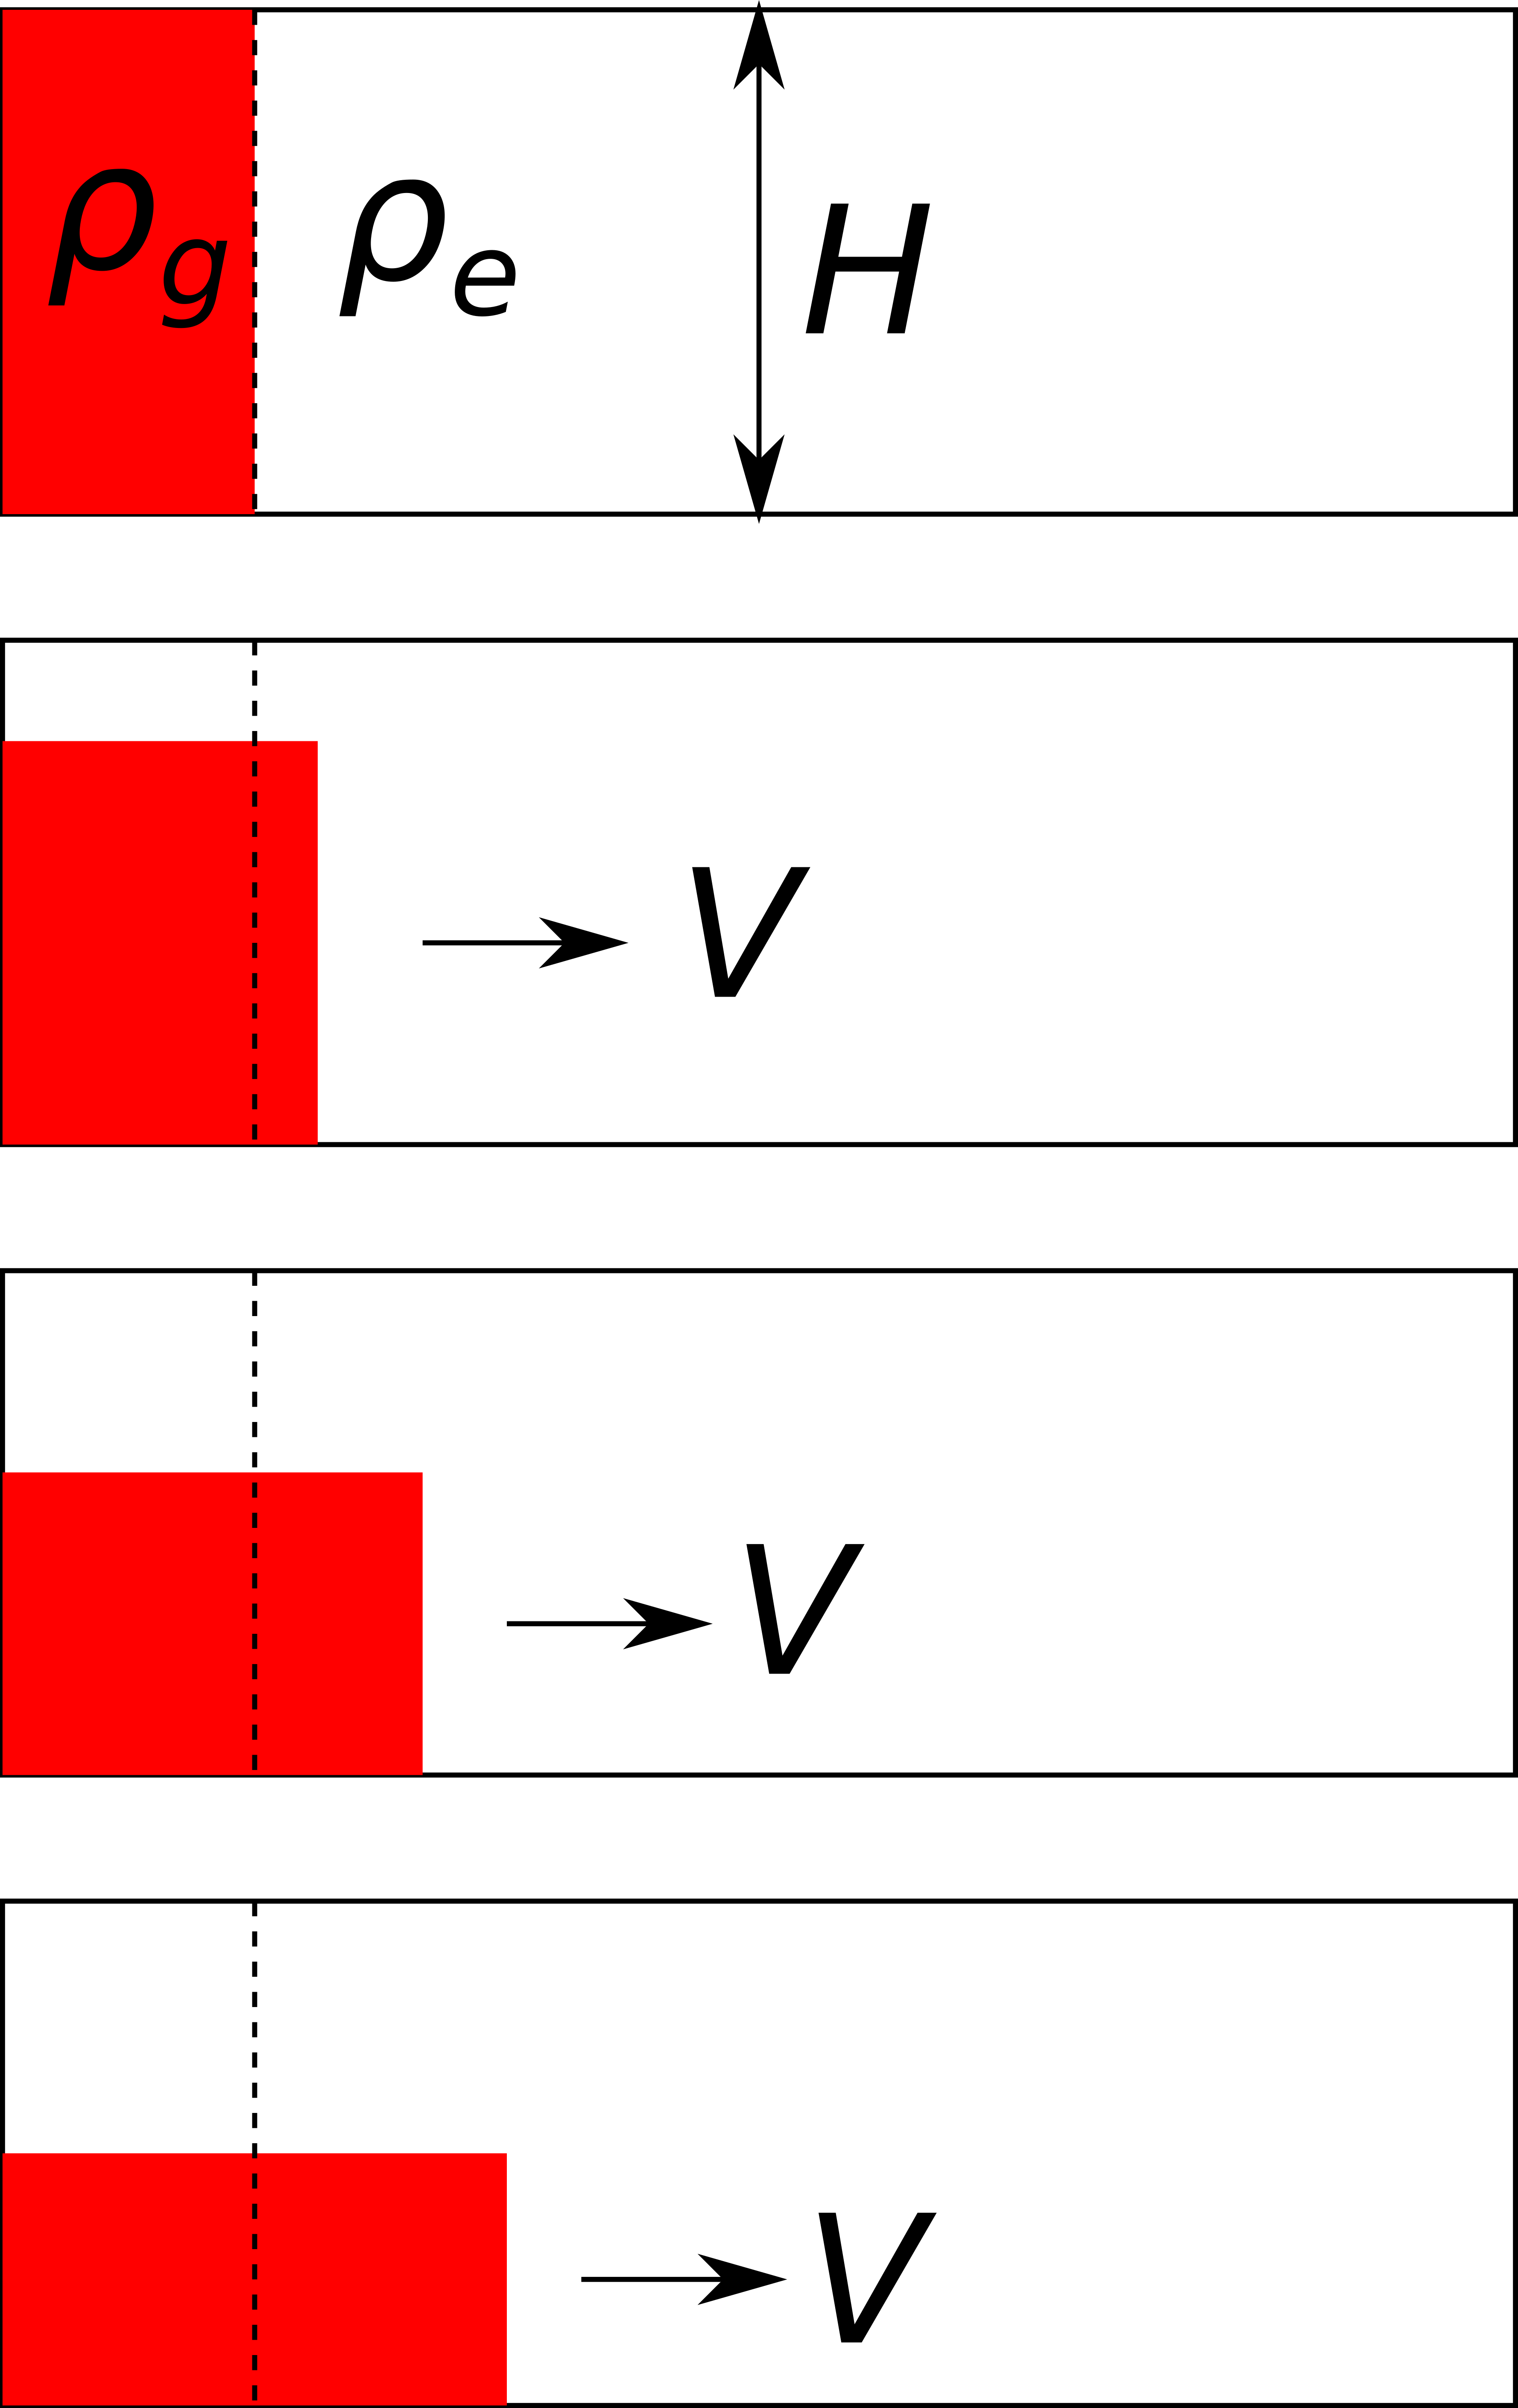
\includegraphics[width=0.7\textwidth]{box_model.png}$$
      
    \end{column}

    \begin{column}{0.59\paperwidth}

      Assume:

      \begin{itemize}
      \item Volume of current is conserved \\
      \item Current is always rectangular \\
      \item Energy is always conserved$^{*}$ \\
      \end{itemize}

      Energy balance between kinetic energy and change in GPE shows

      $$ V = \left(\frac{(\rho_{\text{c}} - \rho_{\text{e}}) g H}{2 \rho_{\text{c}}} \right)^{1/2}$$

      \vspace{0.5cm}
      
      $^{*}$ Means assume energy only exists as kinetic of GPE. What other types of energy are there?
      
    \end{column}

  \end{columns}

\end{frame}
%-----------------------------------------------
\begin{frame}
  \frametitle{Gravity currents - Reduced gravity}

  \begin{columns}[t]

    \begin{column}{0.4\paperwidth}

      \vspace{-0.5cm}
      
      $$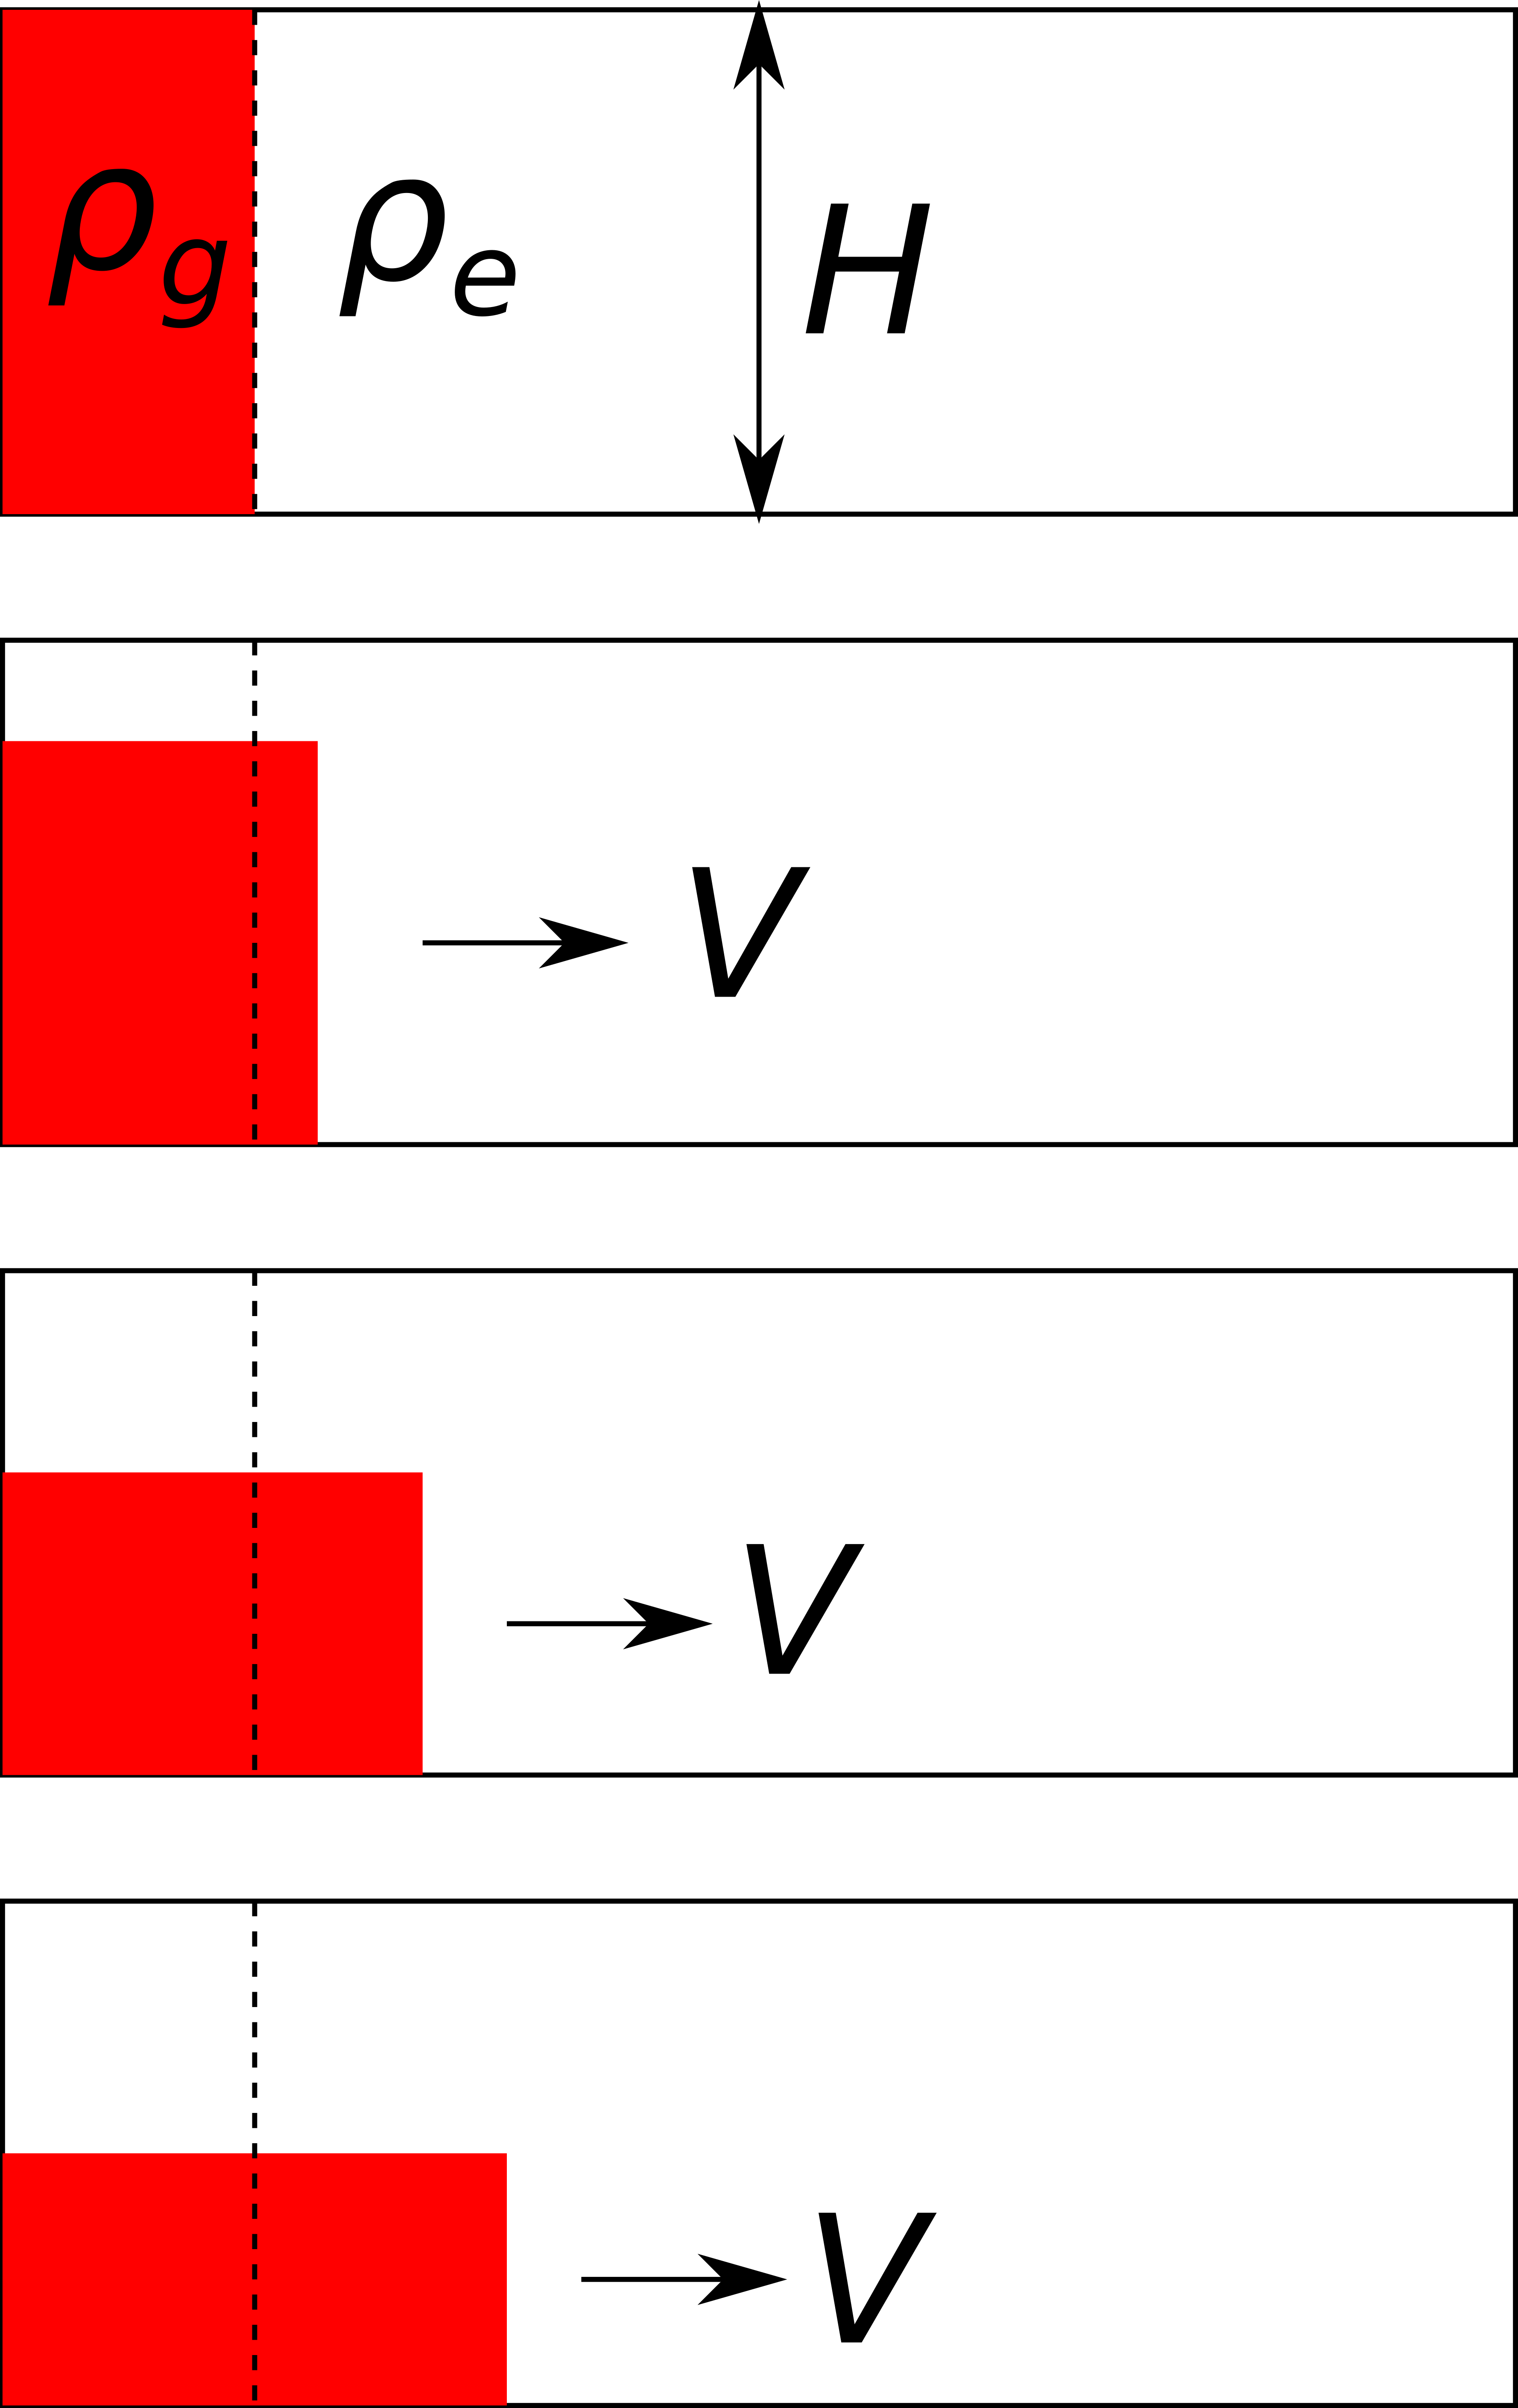
\includegraphics[width=0.7\textwidth]{box_model.png}$$
      
    \end{column}

    \begin{column}{0.59\paperwidth}

      If envrionment is air, then often $\rho_{\text{e}} \ll \rho_{\text{c}}$ \\
      
      $$ V = \left(\frac{(\rho_{\text{c}} - \rho_{\text{e}}) g H}{2 \rho_{\text{c}}} \right)^{1/2} \approx \frac{(g H)^{1/2}}{2} $$

      Therefore, we see that $(\rho_{\text{c}} - \rho_{\text{e}}) / \rho_{\text{c}}$ is factor by which envrionmental fluid reduced gravitational acceleration \\

      Define \textbf{reduced gravity}:

      $$ g' = \frac{\rho_{\text{c}} - \rho_{\text{e}}}{\rho_{\text{c}}}$$

      So generally:

      $$ V = \frac{(g'H)^{1/2}}{2} $$
    \end{column}

  \end{columns}

\end{frame}
%-----------------------------------------------
\begin{frame}
  \frametitle{Gravity currents - Froude number}

  \textbf{Froude number}:

  $$ \text{Fr} = \frac{V}{(g'H)^{1/2}} $$

  Represents ratio of inertial ($U$) to buoyancy ($(g'H)^{1/2}$) forces \\

  \vspace{1cm}
  
  For an ideal gravity current $V = (g' H)^{1/2} / 2$ so:

  $$ \text{Fr} = \frac{1}{2} $$

  Measuring $\text{Fr}$ gives a means of testing model assumptions \\

  
\end{frame}
%-----------------------------------------------
\begin{frame}
  \frametitle{Dimensionless numbers}

  \centering
  \begin{tabular}{|c|c|c|c|}
    \hline
    Froude & $\text{Fr}$ & $\frac{V}{(g'H)^{1/2}}$ & Inertia and buoyancy forces\\
    Capillary & $\text{Ca}$ & $\frac{\eta V r}{\sigma}$ & Viscous and surface tension forces \\
    \hline
  \end{tabular}

  Can use values of these quantities to define different fluid dynamical regimes \\

  \textbf{Reynolds number} - Ratio of inertial and viscous forces within a fluid \\

  $$ \text{Re} = \frac{\rho V L}{\eta}$$

  \begin{columns}[t]

    \begin{column}{0.5\paperwidth}

      \centering
      
      $\rho$ = Fluid density \\

      $V$ = Fluid velocity
      
    \end{column}

    \begin{column}{0.5\paperwidth}

      \centering
      
      $L$ = Lengthscale \\

      $\eta$ = Viscosity 
    \end{column}
  \end{columns}
  
\end{frame}
%-----------------------------------------------
\begin{frame}
  \frametitle{Reynolds number}

  $$ \text{Re} = \frac{\rho V L}{\eta}$$

  \vspace{-1cm}
  
  \begin{columns}[t]

    \begin{column}{0.5\paperwidth}

      \centering
      
      $$ \text{Re} \ll \text{Re}_{\text{c}}$$

      \textbf{Laminar flow}

      Fluid particles follow smooth paths in layers, with little or no mixing between different layers \\

      $$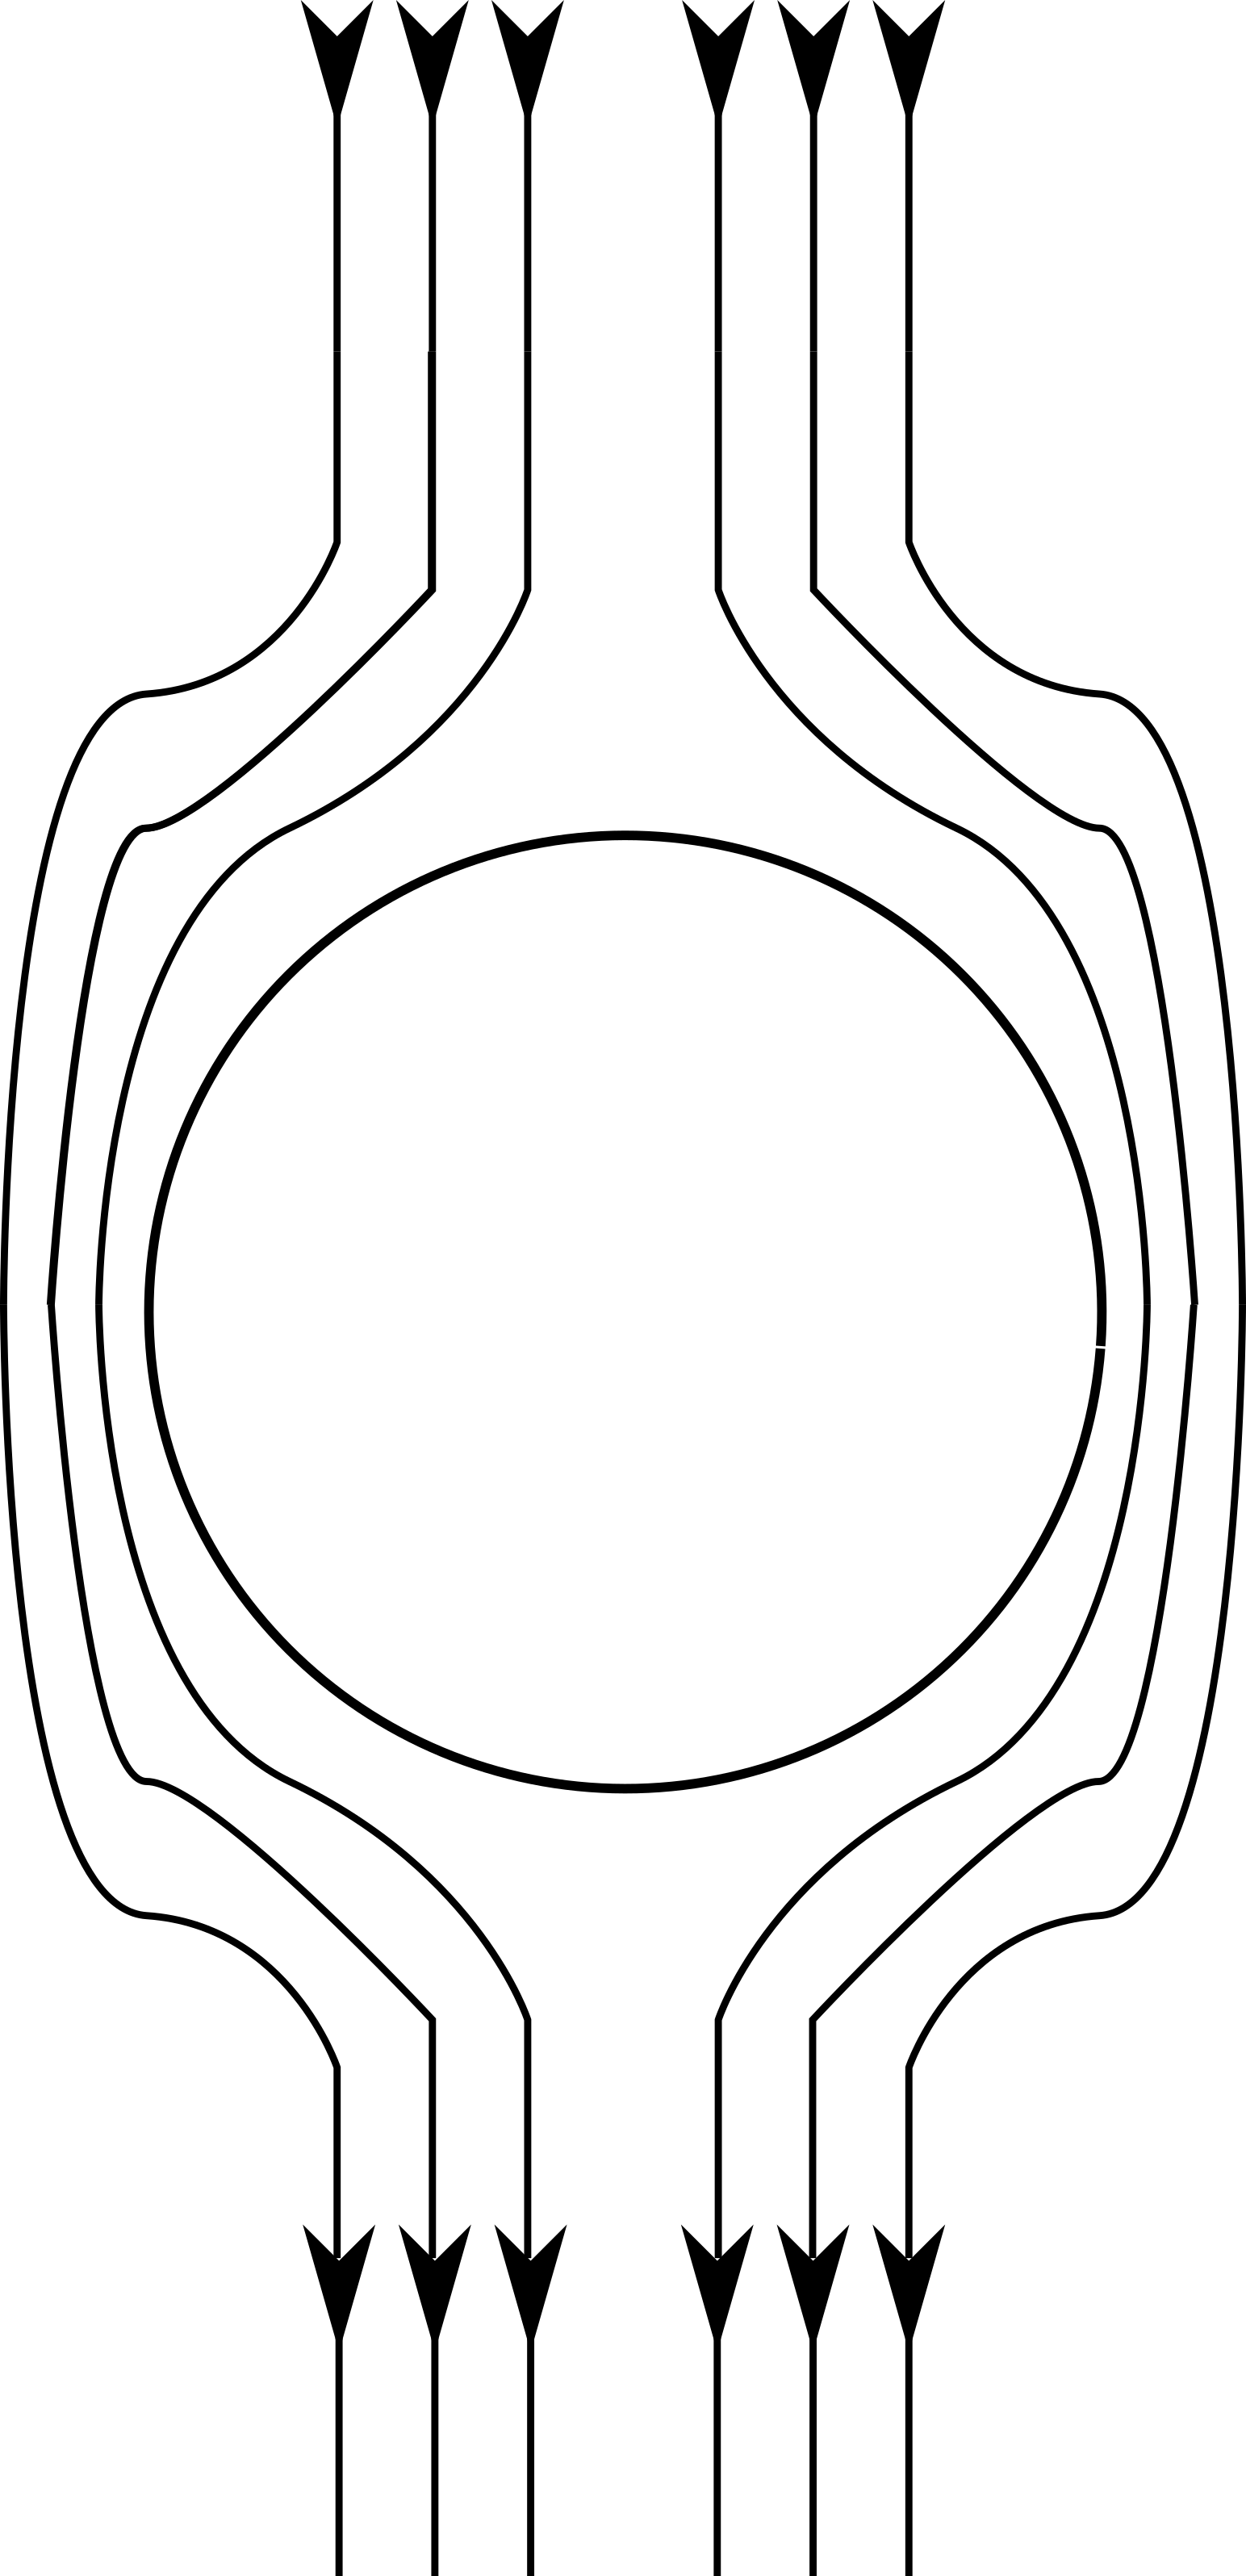
\includegraphics[width=0.45\textwidth, angle=90]{laminar.png}$$
      
    \end{column}

    \begin{column}{0.5\paperwidth}

      \centering
      
      $$ \text{Re} \gg \text{Re}_{\text{c}}$$

      \textbf{Turbulent flow}

      Chaotic changes in pressure and flow velocity, generating unsteady vortices \\

      \vspace{0.5cm}
      
      $$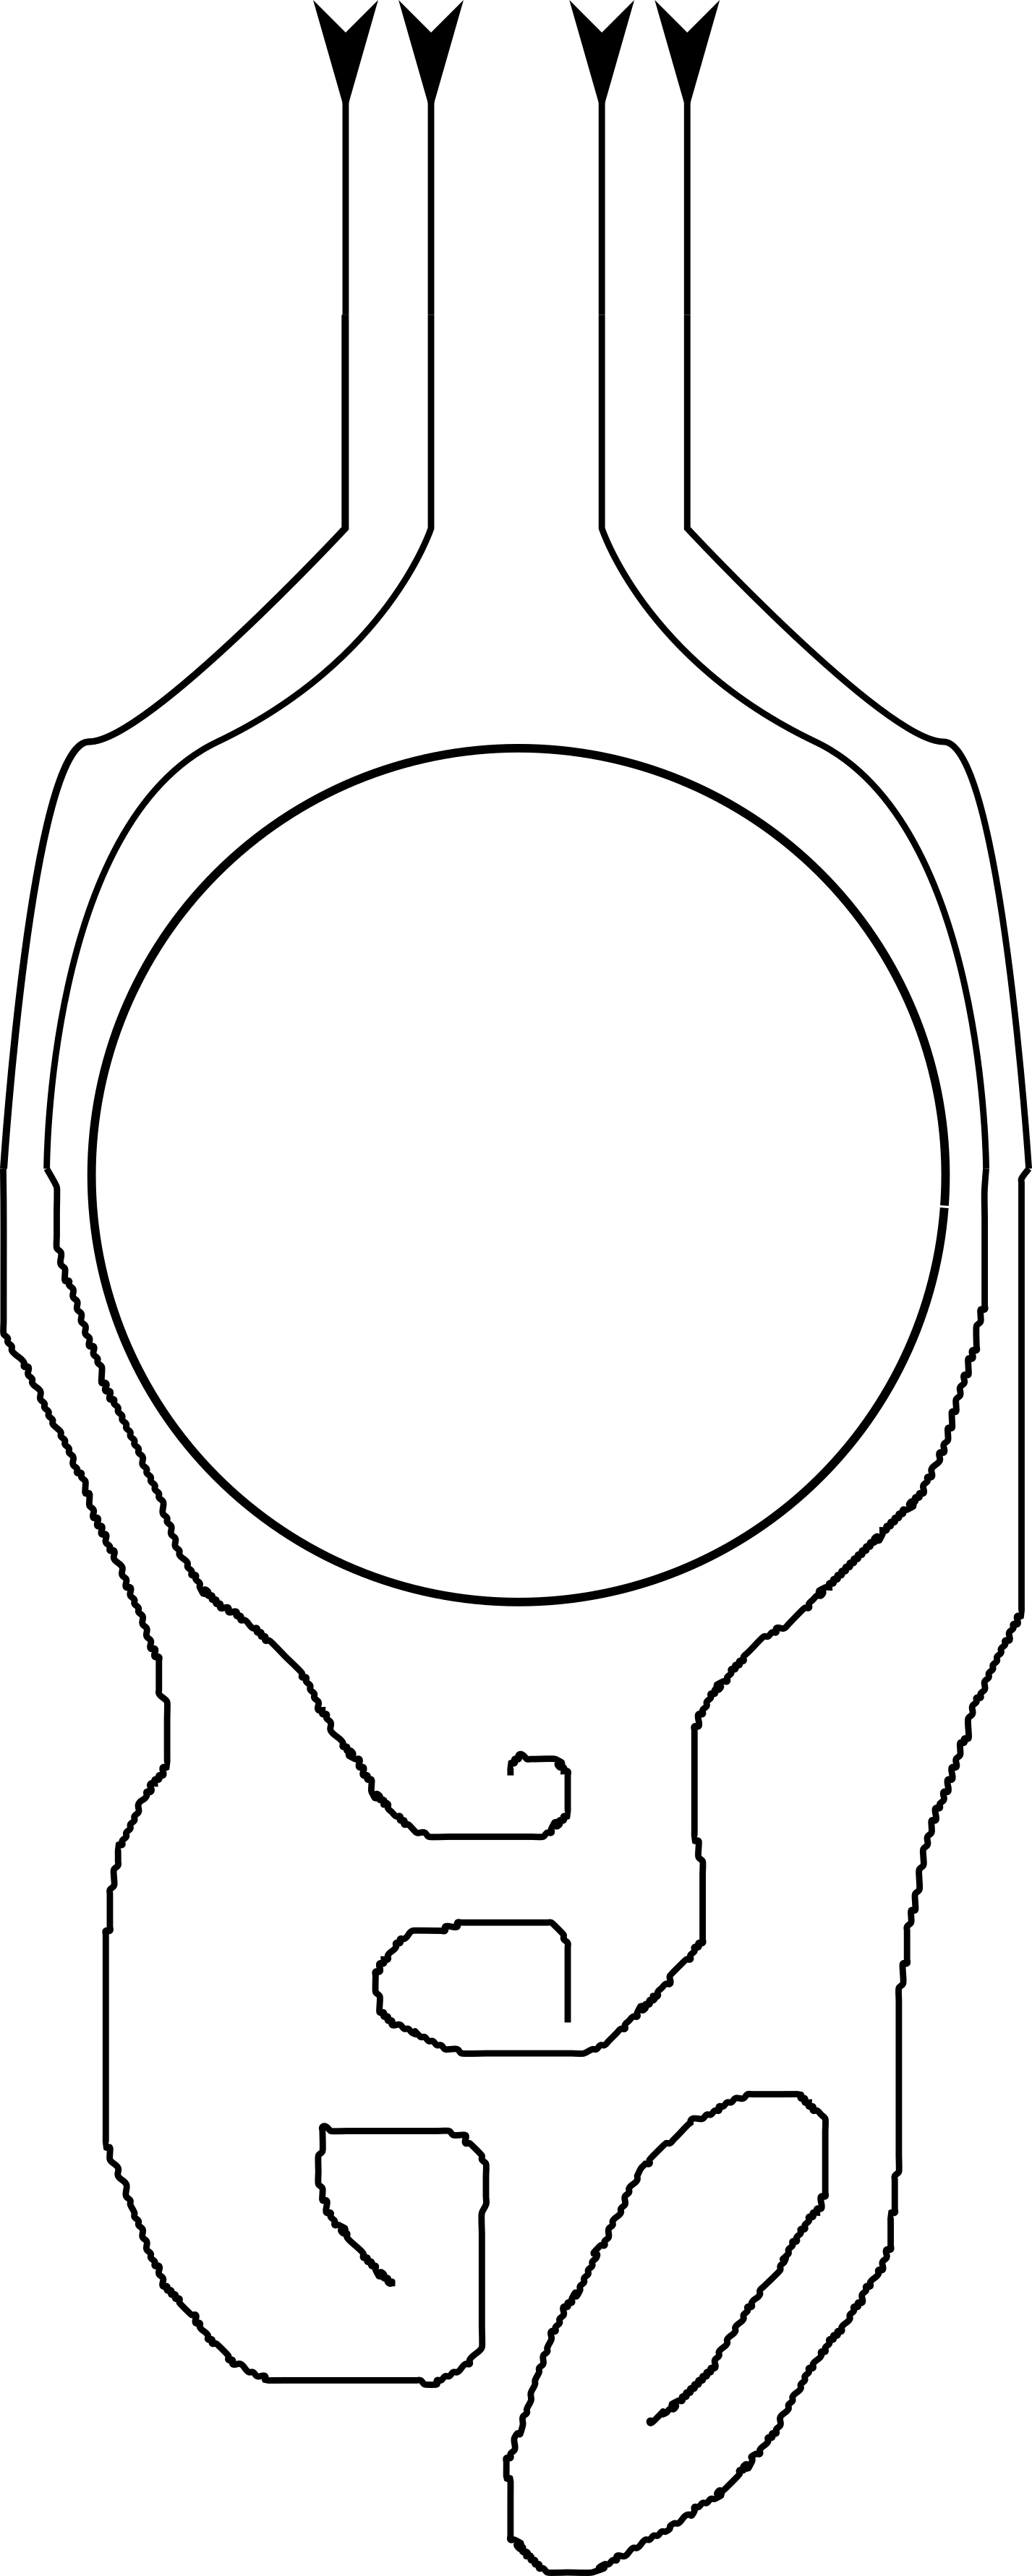
\includegraphics[width=0.4\textwidth, angle=90]{turbulent.png}$$
      
    \end{column}
  \end{columns}
  
\end{frame}
%-----------------------------------------------
\begin{frame}
  \frametitle{Reynolds number}

  What are the Reynolds numbers for these scenarios?
  
  \begin{columns}[t]

    \begin{column}{0.33\paperwidth}

      $$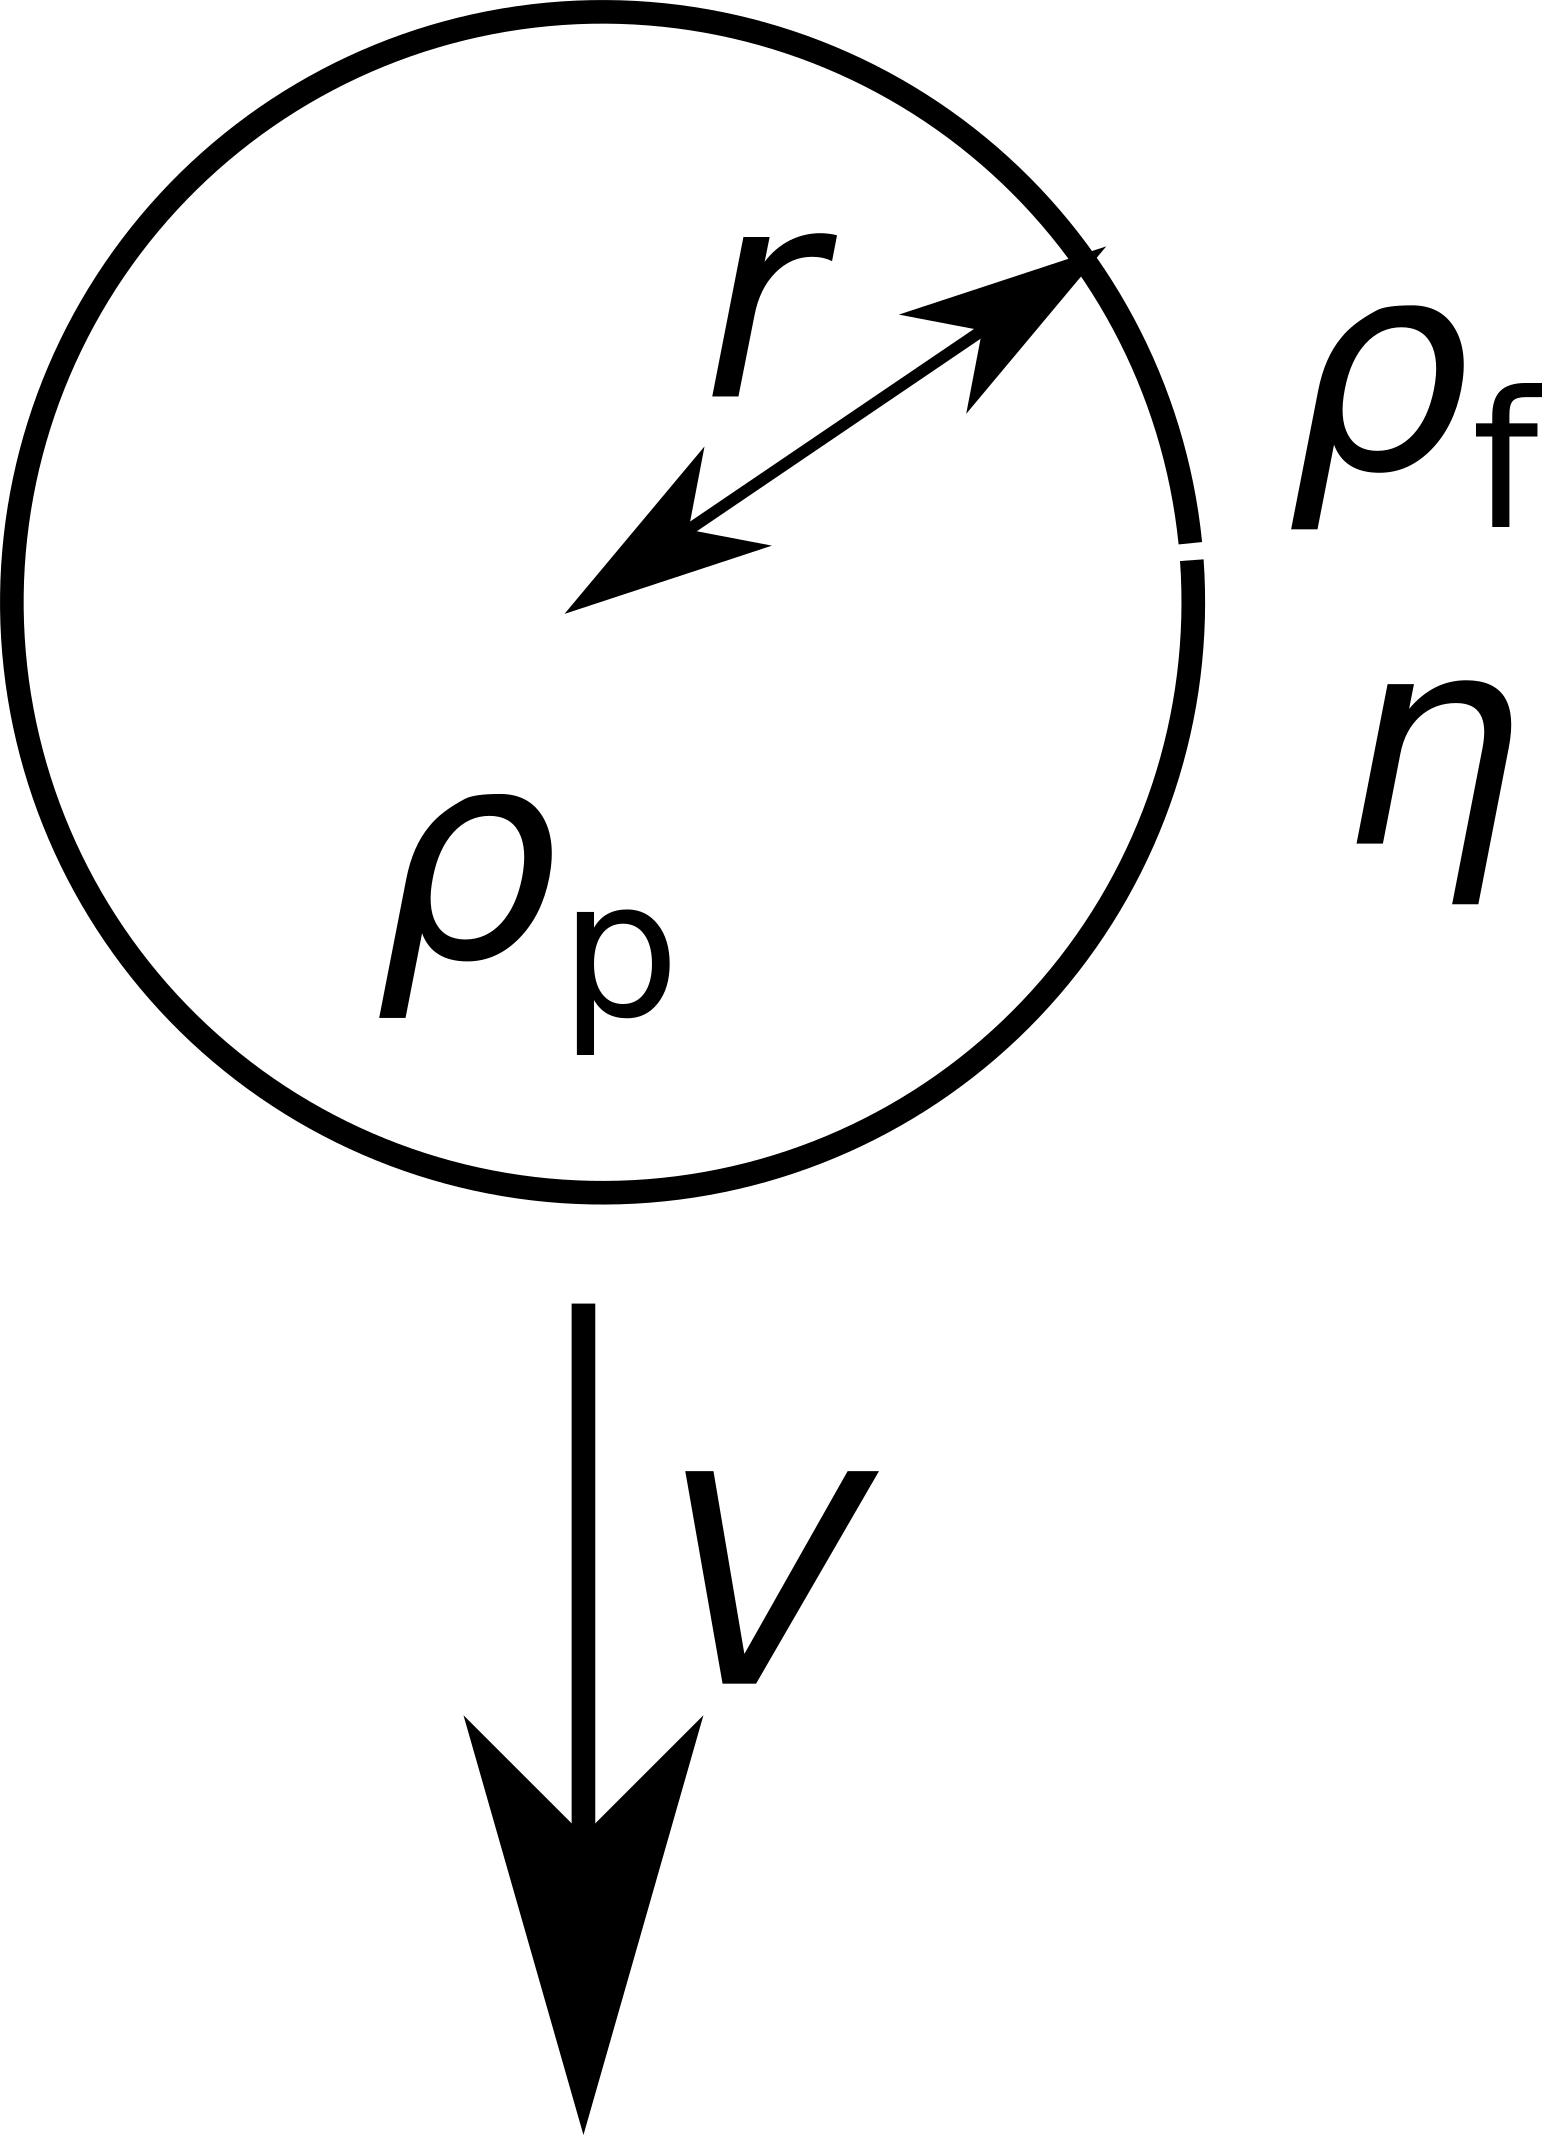
\includegraphics[width=0.9\textwidth]{settling_sphere.png}$$
      
    \end{column}

    \begin{column}{0.33\paperwidth}

      $$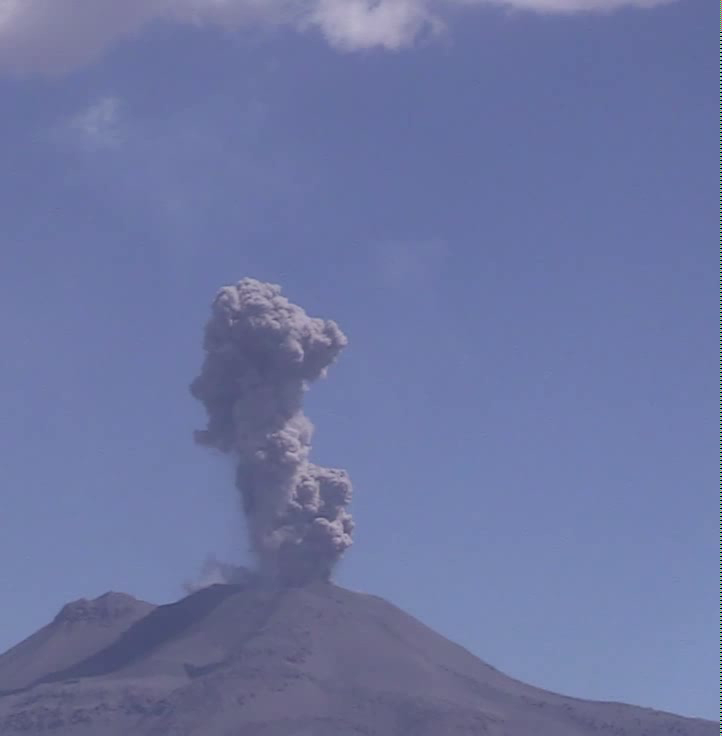
\includegraphics[width=0.9\textwidth]{visible.png}$$
      
    \end{column}

    \begin{column}{0.33\paperwidth}

      $$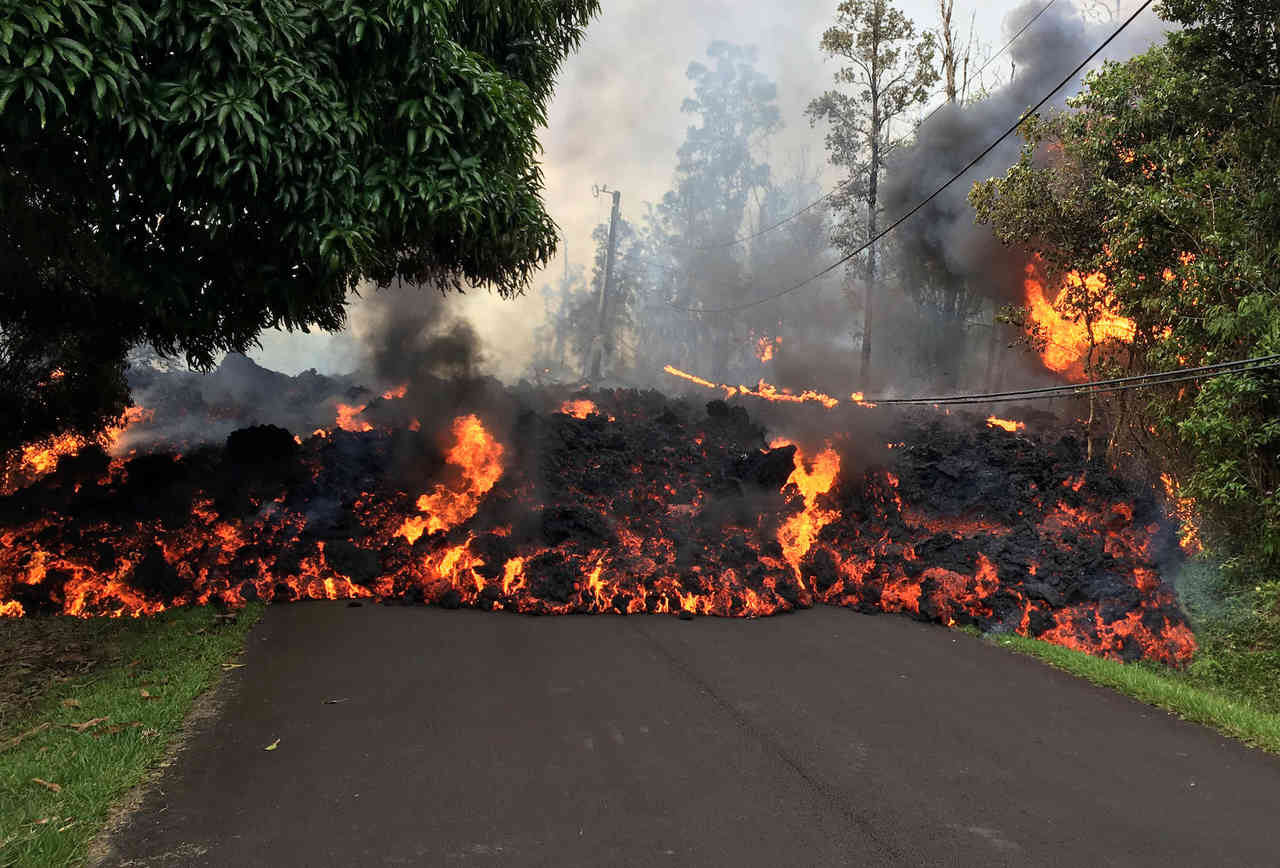
\includegraphics[width=0.9\textwidth]{lava.jpg}$$
      
    \end{column}
  \end{columns}
  
\end{frame}
%-----------------------------------------------
\begin{frame}
  \frametitle{Low-Reynolds number gravity currents}

  \begin{columns}[t]

    \begin{column}{0.66\paperwidth}

      \vspace{-1cm}
      
      $$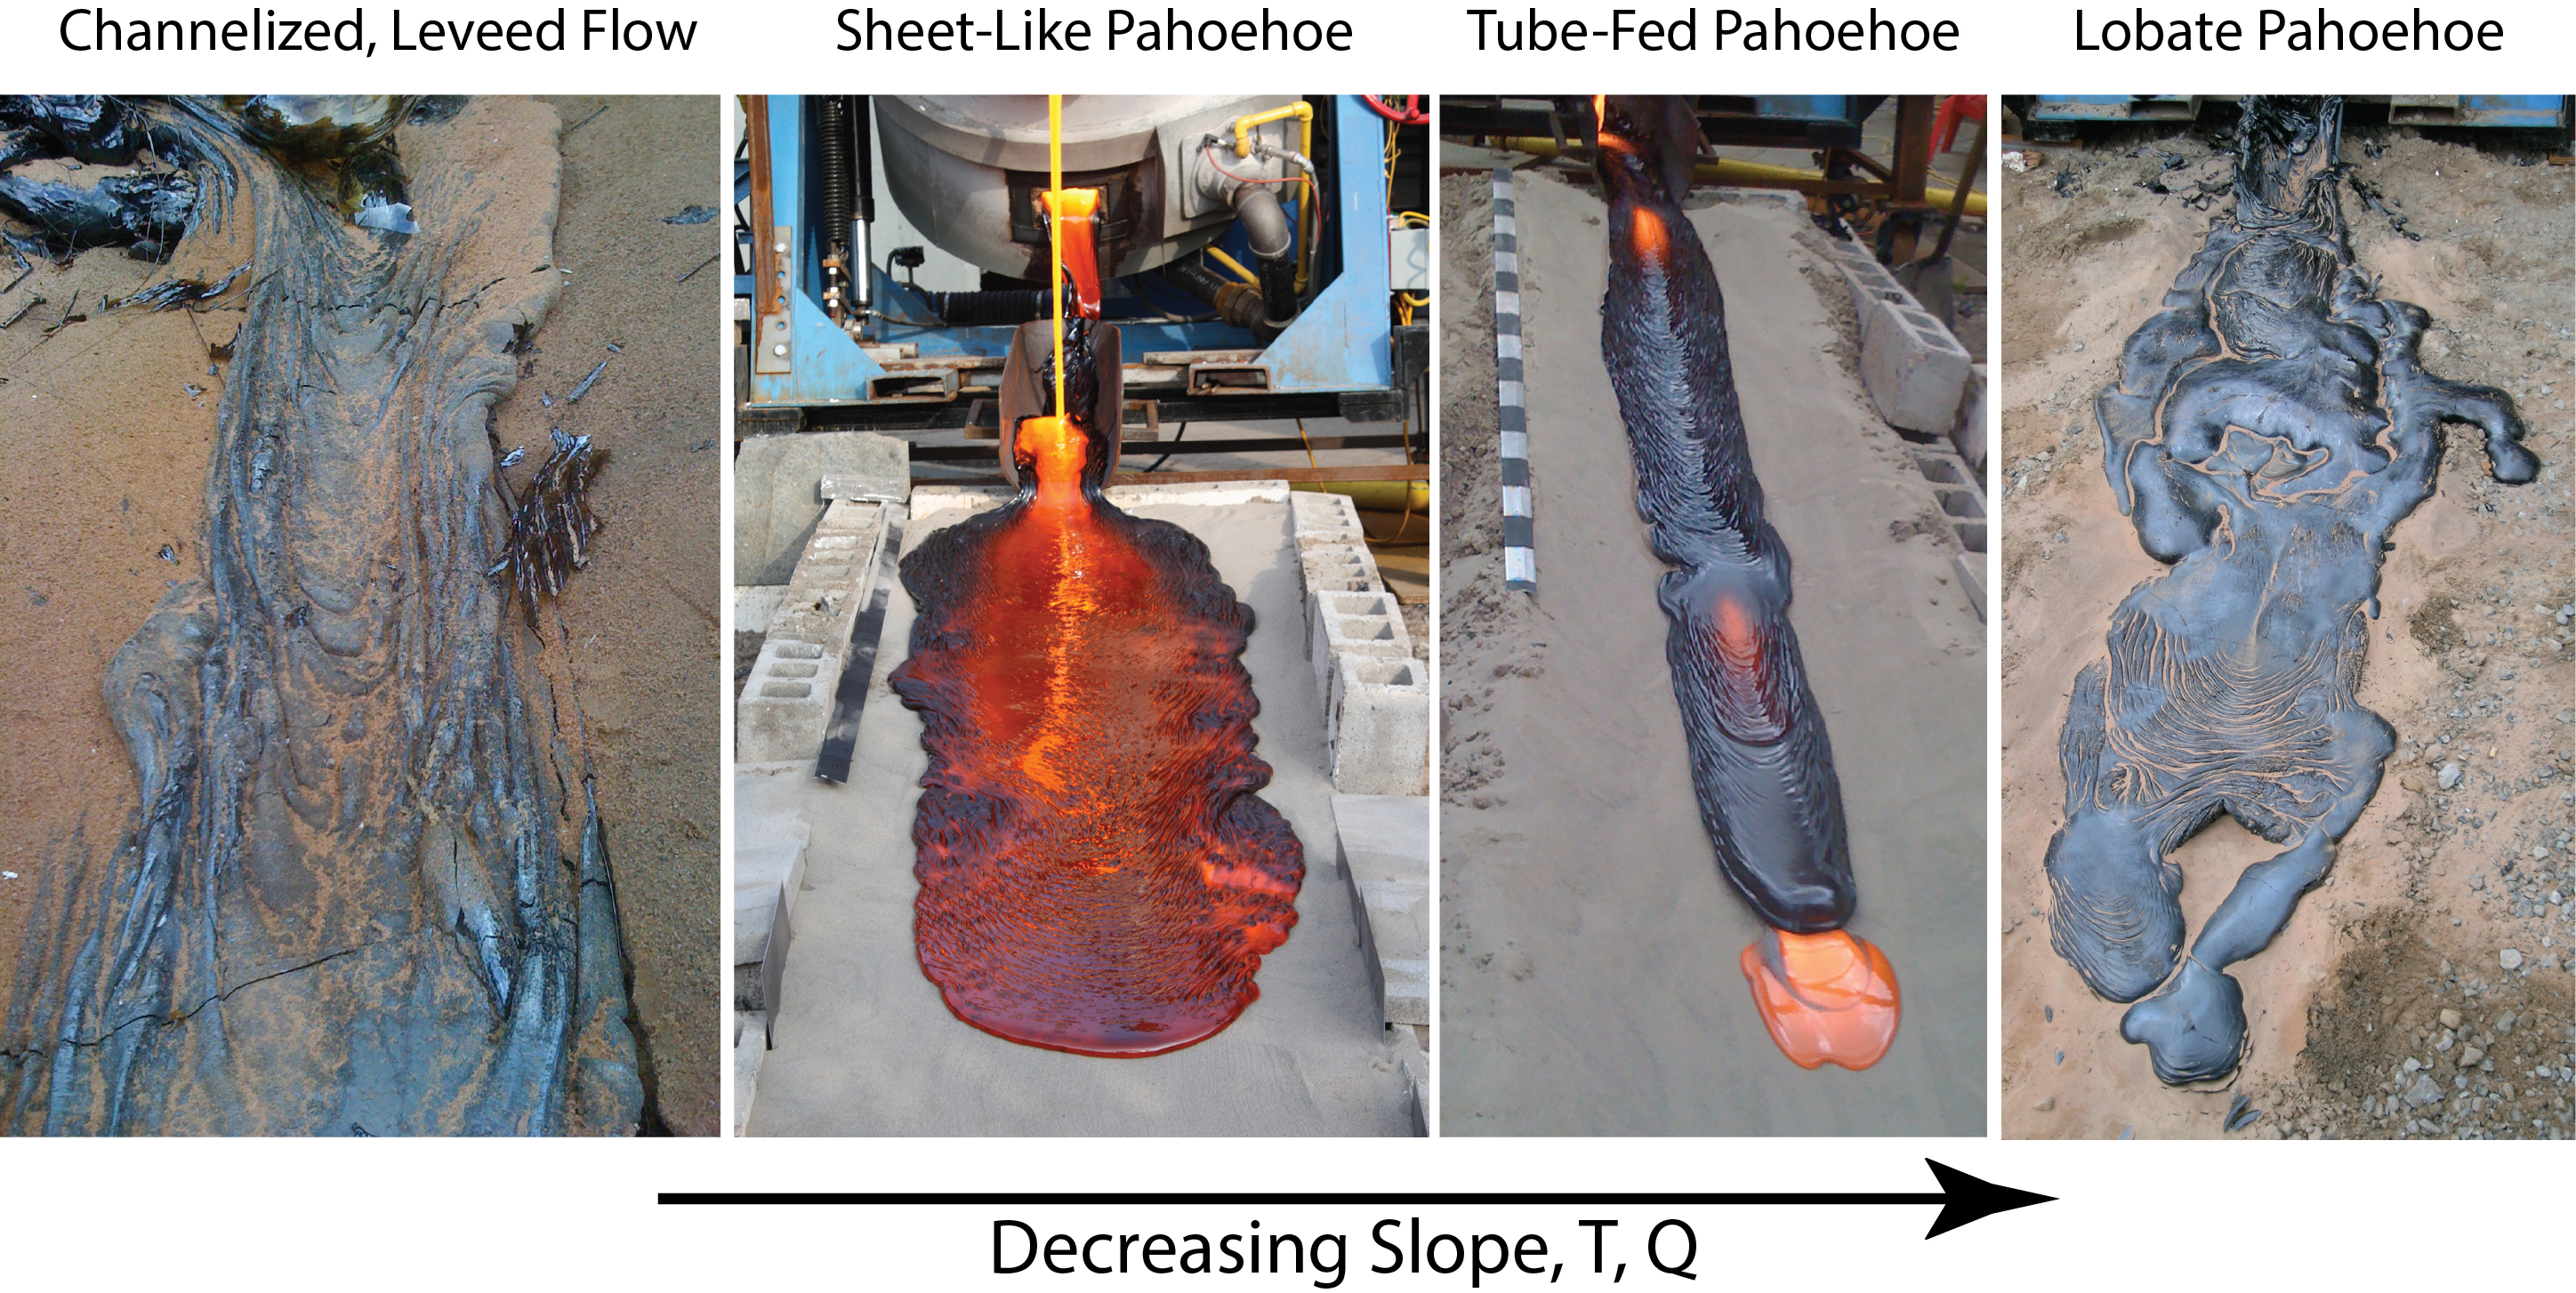
\includegraphics[width=0.9\textwidth]{lava_morph.jpg}$$
      
    \end{column}

    \begin{column}{0.33\paperwidth}

      For fixed release volume, viscous dissipation continuosly reduces $V$ \\

      \vspace{0.5cm}
      
      Varying slope angle and flow rate produces different flow morphologies \\
    \end{column}
  \end{columns}

  For a 2D current:

  \begin{columns}[t]

    \begin{column}{0.66\paperwidth}

      \vspace{-1cm}
      
      $$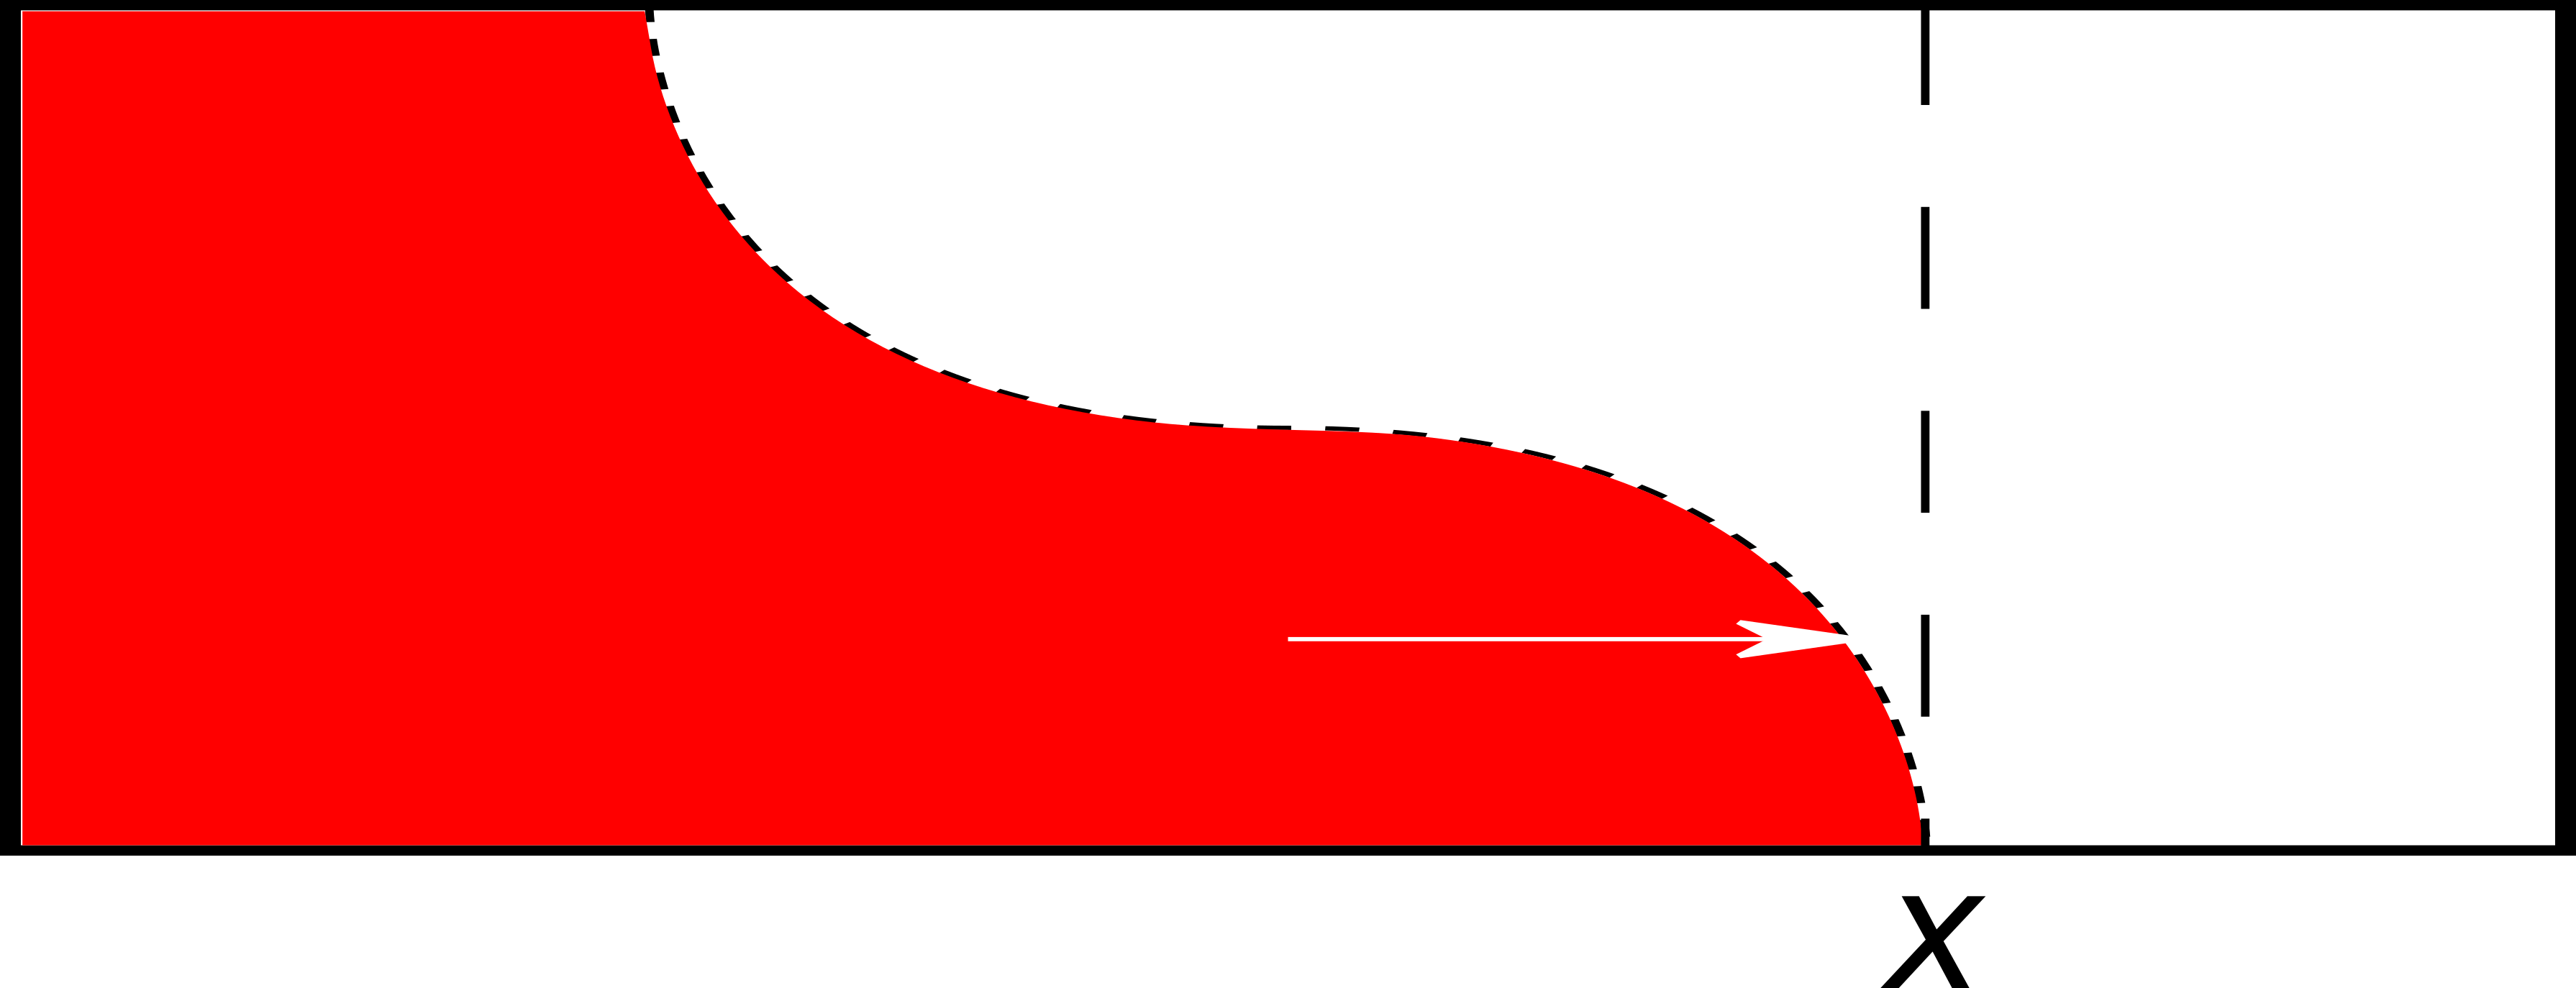
\includegraphics[width=0.9\textwidth]{viscous_grav_curr}$$
      
    \end{column}

    \begin{column}{0.33\paperwidth}

      $$ x \sim t^{4/5} $$
    \end{column}
  \end{columns}
  
  
\end{frame}
%-----------------------------------------------
\begin{frame}
  \frametitle{High-Reynolds number gravity currents}

  For $\text{Re} > 1000$, $\text{Re}$ has no effect on flow \\
  
  Can neglect viscous dissipation $\implies V = (g'H)^{1/2}/2$

  $$ g' = 0.06 $$
  \movie{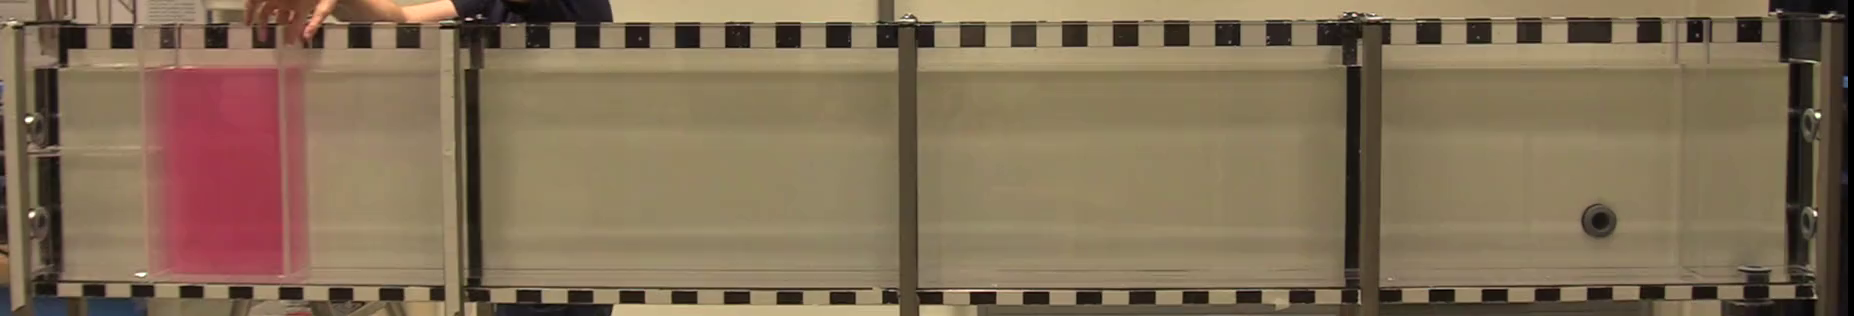
\includegraphics[width=\textwidth]{GC3.png}}{GC3.mp4}

  $$ g' = 0.16 $$  
  \movie{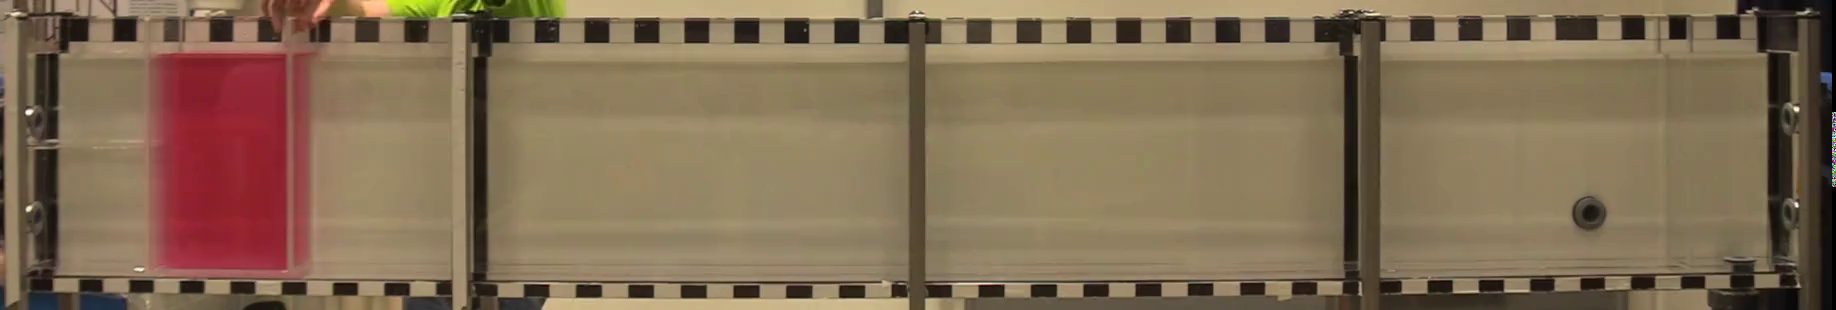
\includegraphics[width=\textwidth]{GC9.png}}{GC9.mp4}
  
\end{frame}
%-----------------------------------------------
\begin{frame}
  \frametitle{High-Reynolds number gravity currents - mixing}

  \begin{columns}[t]

    \begin{column}{0.66\paperwidth}

      \vspace{-1cm}
      
      $$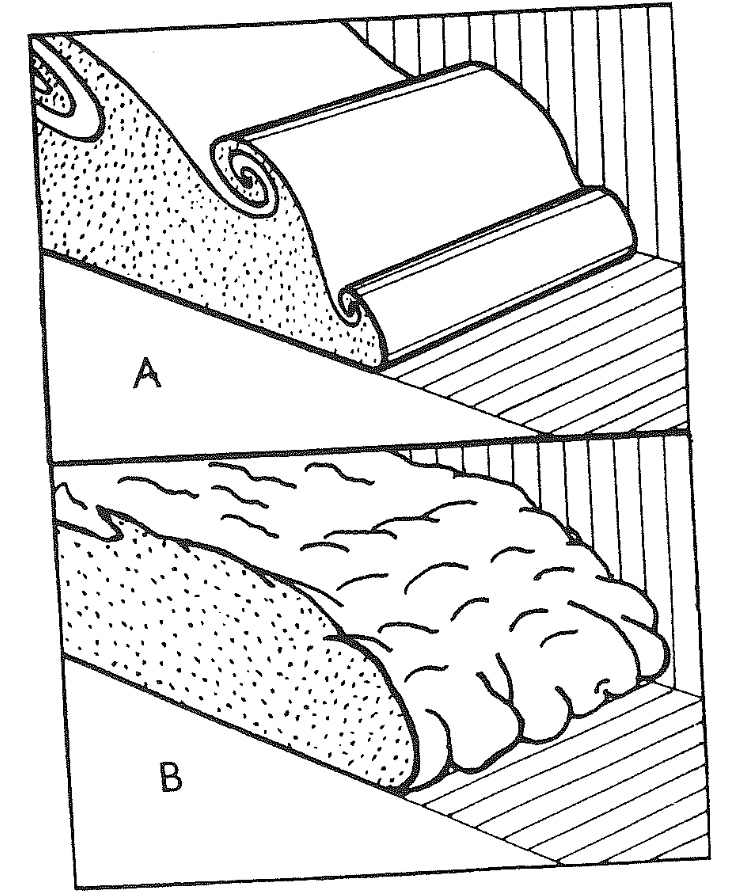
\includegraphics[width=0.6\textwidth]{mixing.png}$$
      
    \end{column}

    \begin{column}{0.33\paperwidth}

      Two types of mixing:

      \begin{itemize}
      \item \textbf{Billowing} - Formed by shear between current and environment \\
      \item \textbf{Lobes and clefts} - Formed by interaction with ground at contact line \\
      \end{itemize}
    \end{column}

  \end{columns}

  Mixing in fluid reduced density contrast 
  
\end{frame}
%-----------------------------------------------
\begin{frame}
  \frametitle{Constant volume release - Constant speed phase}

  \movie{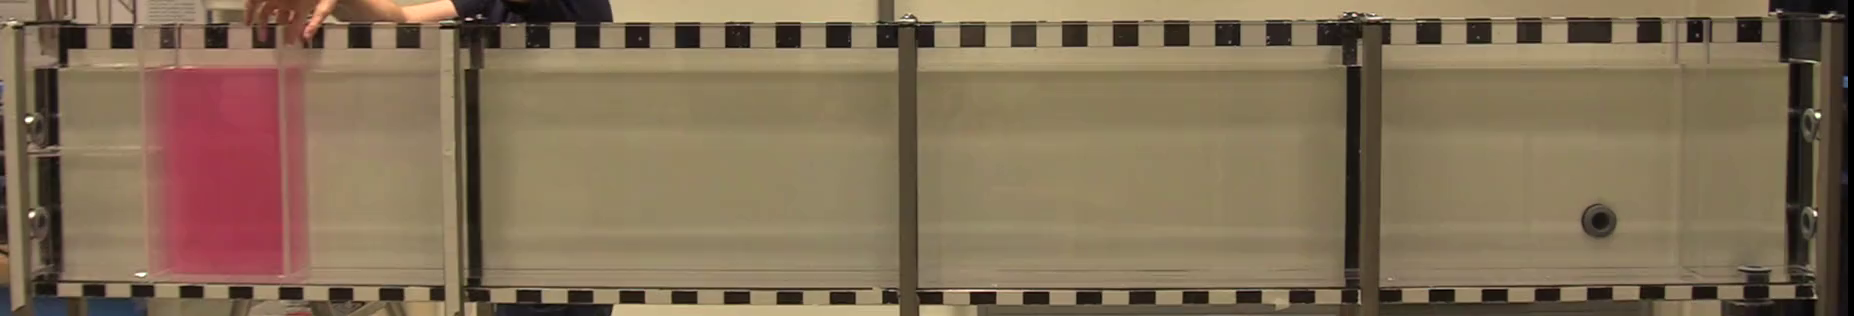
\includegraphics[width=\textwidth]{GC3.png}}{GC3.mp4}

  \begin{columns}[t]

    \begin{column}{0.5\paperwidth}

      $$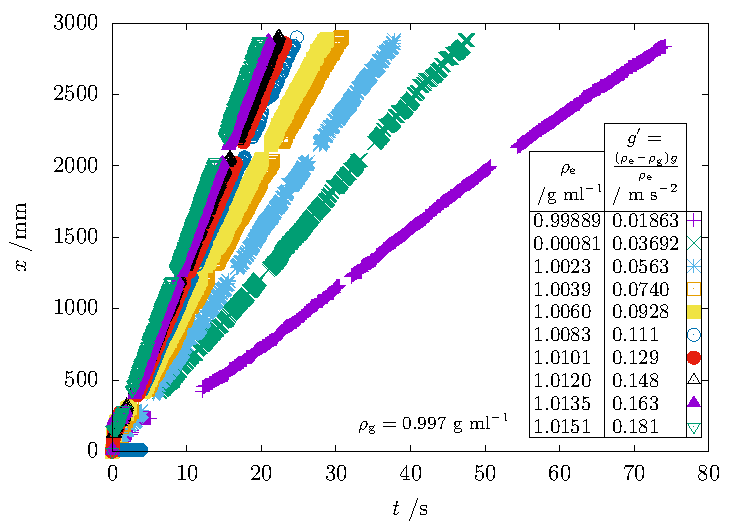
\includegraphics[width=0.9\textwidth]{front_pos.pdf}$$
      
    \end{column}

    \begin{column}{0.5\paperwidth}

      $$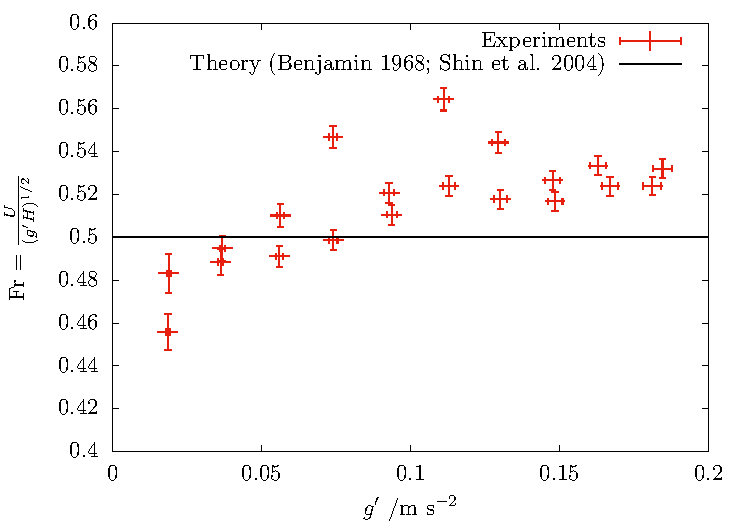
\includegraphics[width=0.9\textwidth]{Froude.pdf}$$
      
    \end{column}

  \end{columns}
  
\end{frame}
%-----------------------------------------------
\begin{frame}
  \frametitle{Constant volume release - Self-similar phase}

  $$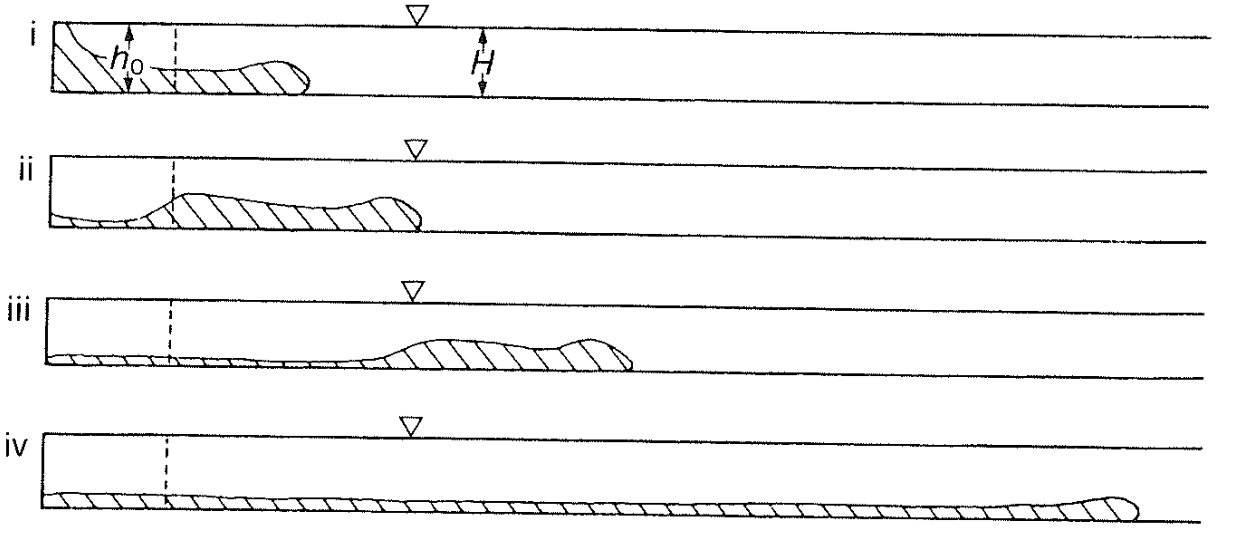
\includegraphics[width=0.9\textwidth]{self_similar_bore.png}$$

  \vspace{-0.5cm}
  
  \begin{columns}[t]

    \begin{column}{0.33\paperwidth}

      \centering Constant speed

      \vspace{-0.5cm}
      
      $$ x \sim t $$
    \end{column}

    \begin{column}{0.33\paperwidth}

      \centering Self-similar

      \vspace{-0.5cm}
      
      $$ x \sim t^{2/3} $$
    \end{column}

    \begin{column}{0.33\paperwidth}

      \centering Viscous

      \vspace{-0.5cm}
      
      $$ x \sim t^{1/5} $$
    \end{column}
    
  \end{columns}
\end{frame}
%-----------------------------------------------
\begin{frame}
  \frametitle{Constant volume release - Radial collapse}

  $$ r \sim t^{1/2} $$
  
  $$\includegraphics[width=0.7\textwidth]{radial_curr.png}$$

\end{frame}
%-----------------------------------------------

\begin{frame}
  \frametitle{Constant radial volume flow}

  $$ r \sim Q^{1/3} t^{1/2} $$
  
  $$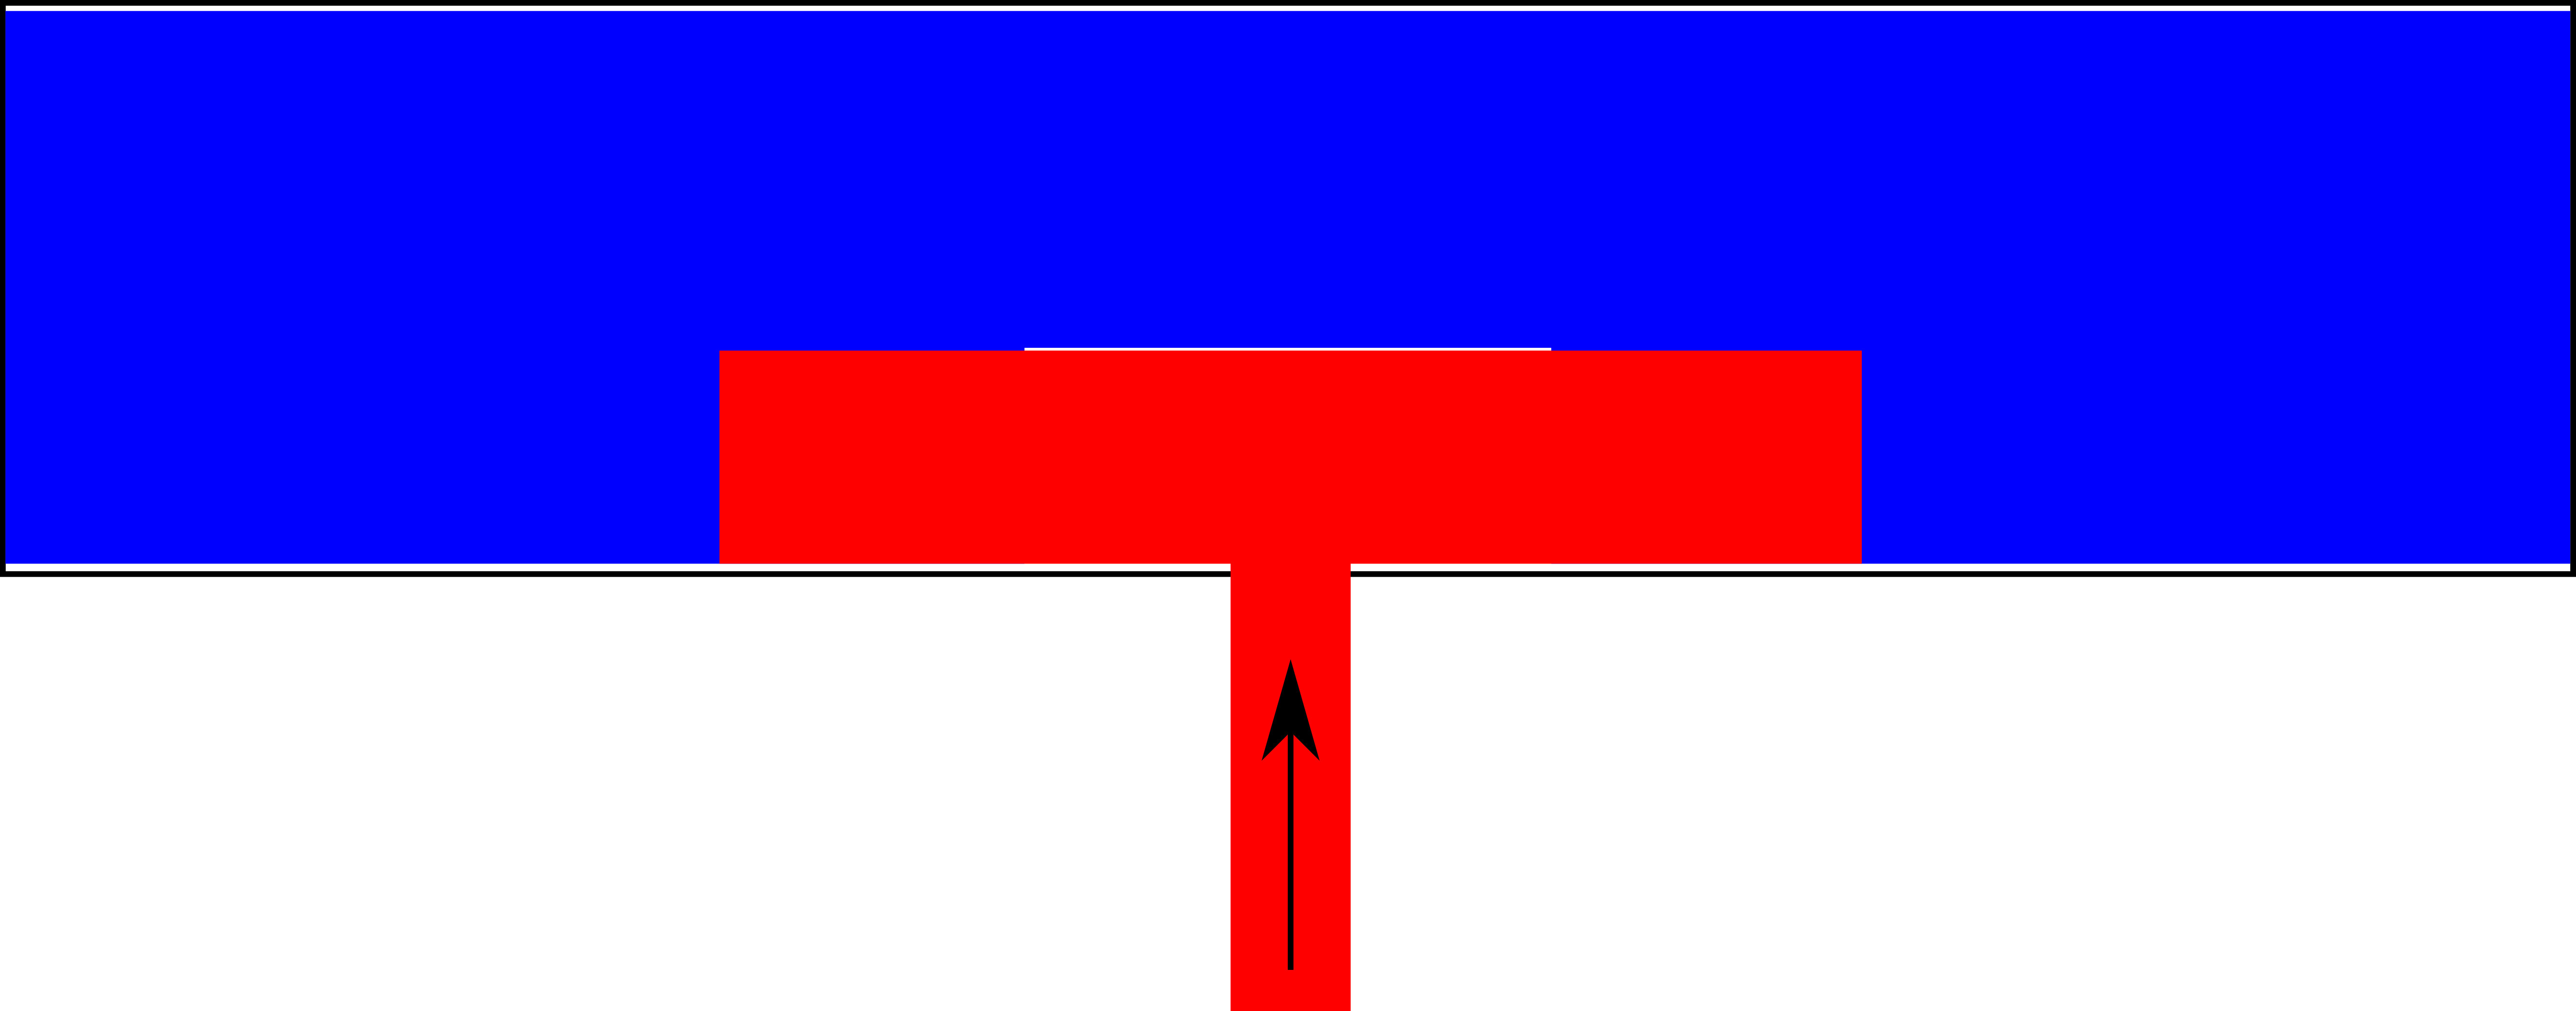
\includegraphics[width=0.7\textwidth]{radial_flux.png}$$

\end{frame}
%-----------------------------------------------



\end{document}
